\documentclass[11pt,a4paper]{article}

% ── Packages (only those available on this installation) ──────────────────────
\usepackage[margin=2.5cm]{geometry}
\usepackage{amsmath,amssymb}
\usepackage{graphicx}
\usepackage{booktabs}
\usepackage{longtable}
\usepackage{array}
\usepackage{xcolor}
\usepackage{hyperref}
\usepackage{caption}
\usepackage{subcaption}
\usepackage{enumitem}
\usepackage{microtype}
\usepackage{listings}
\usepackage{float}
\usepackage{placeins}

% ── Figure path ───────────────────────────────────────────────────────────────
\graphicspath{{figures/}}

% ── Hyperref setup ────────────────────────────────────────────────────────────
\hypersetup{
  colorlinks = true,
  linkcolor  = blue!70!black,
  citecolor  = green!50!black,
  urlcolor   = blue!70!black,
}

% ── Custom commands ───────────────────────────────────────────────────────────
\newcommand{\numu}{$\nu_\mu$}
\newcommand{\numubar}{$\bar{\nu}_\mu$}
\newcommand{\ccpip}{$\mathrm{CC}\pi^{\pm}$}
\newcommand{\pmu}{$p_\mu$}
\newcommand{\ppi}{$p_\pi$}
\newcommand{\costhmu}{$\cos\theta_\mu$}
\newcommand{\costhpi}{$\cos\theta_\pi$}
\newcommand{\thmupi}{$\theta_{\mu\pi}$}
\newcommand{\uboone}{MicroBooNE}
\newcommand{\GeVc}{\,\text{GeV}\!/c}
\newcommand{\pot}{\,\text{POT}}
\newcommand{\cm}{\,\text{cm}}

% inline math shorthand so they work inside math mode too
\newcommand{\pmuM}{p_\mu}
\newcommand{\ppiM}{p_\pi}
\newcommand{\cthmuM}{\cos\theta_\mu}
\newcommand{\cthpiM}{\cos\theta_\pi}
\newcommand{\thmupM}{\theta_{\mu\pi}}

% ── Listings (C++ snippets) ───────────────────────────────────────────────────
\lstset{
  language=C++,
  basicstyle=\ttfamily\small,
  keywordstyle=\bfseries\color{blue!70!black},
  commentstyle=\itshape\color{gray},
  backgroundcolor=\color{gray!10},
  frame=single,
  framerule=0.4pt,
  numbers=none,
  breaklines=true,
}

% ── Table column helpers ──────────────────────────────────────────────────────
\newcolumntype{C}[1]{>{\centering\arraybackslash}p{#1}}
\newcolumntype{R}[1]{>{\raggedleft\arraybackslash}p{#1}}
\newcolumntype{L}[1]{>{\raggedright\arraybackslash}p{#1}}

% Let TeX stretch spacing on hard-to-break lines (long \texttt paths/code) to keep
% text out of the margin.
\emergencystretch=3em

% ─────────────────────────────────────────────────────────────────────────────


% ---- cross-document references to the analysis note ----
\usepackage{xr}
\externaldocument[N-]{analysis_note}
\newcommand{\noteref}[2]{#1~\ref{N-#2} of the analysis note}

\begin{document}

\begin{titlepage}
\centering
\vspace*{2cm}
{\LARGE\bfseries Technical Validation Supplement\par}
\vspace{0.5cm}
{\large Measurement of $\nu_\mu + \bar{\nu}_\mu$ Charged-Current Single Pion
Production on Argon in the NuMI Beam\par}
\vspace{0.8cm}
{\large Companion to the analysis note\par}
\vspace{0.5cm}
{\normalsize Draft 1.5, release 2026-09-06 \textperiodcentered\ document revision 2026-09-07\par}
\vspace{0.15cm}
{\footnotesize\ttfamily release 2026-09-06 \textperiodcentered\ 51 differential extractions $+$ 6 one-bin totals \textperiodcentered\ blind\par}
\vspace{1.5cm}
{\large Ishanee Pophale, Jarek Nowak\par}
\vspace{0.5cm}
{\normalsize\textit{Lancaster University}\par}
\vspace{2cm}

\begin{abstract}
This supplement holds the validation and diagnostic material for the
$\mathrm{CC}\pi^{\pm}$ NuMI cross-section measurement: the studies that establish
what the measurement can and cannot resolve, the estimators that were tried and
rejected, and the closure tests that qualify the extraction. It is separated from the
analysis note so that the note can state the analysis and its results while the studies
that justify its choices remain available and citable at full length.

The two documents are checked for numerical consistency where current results are
duplicated (\texttt{report/check\_tables.py}, \texttt{xsec\_analyzer/check\_staleness.py});
every number here is from the release named on the title page unless a table says
otherwise. The history of the analysis, the corrections that shaped it and the values
before and after, is in the change log and is not repeated here.

The central results of this supplement are negative ones, and they set the scope of
the measurement.  Charged pions interact hadronically before ranging out, so the
reconstructed momentum saturates near $0.34$~GeV/$c$ and carries little information
about the initial momentum above roughly $0.4$~GeV/$c$.  Every alternative estimator
tried --- golden-pion tagging, multiple Coulomb scattering, calorimetry, multivariate
regression, daughter-energy recovery, and the proton-tagged selection --- fails to
recover it, and a truth-level golden selection performs no better than the classifier,
which places the limitation in the physics rather than in the estimator.  This is what
reduces $p_\pi$ to two bins and $W_{\pi p}$ to an integrated cross section.
\end{abstract}
\end{titlepage}

\tableofcontents
\clearpage


\section{Pion momentum: the range estimator and why it fails}
\label{sec:supp_ppi}

\subsection{The pion-momentum bias and why $p_\pi$ is the worst-conditioned observable}
\label{sec:ppi_bias}

The $p_\pi$ response is the least diagonal of any observable in the analysis. This section
quantifies why, because the cause is physical and sets a floor on what the measurement can
say about the pion momentum spectrum.

\paragraph{Two separate effects, only one of them corrected.}
The reconstructed pion momentum stored in the ntuple,
\texttt{candidate\_pion\_mom\_reco}, is \texttt{trk\_range\_muon\_mom\_v}: a range-based
momentum evaluated under the \emph{muon} mass hypothesis and applied to a pion track. Two
distinct things follow.

First, the mass hypothesis itself biases the estimate low, because for a given range a
pion carries more momentum than a muon. The size is $\sim\!17$--$19\%$ from the CSDA
range scaling, and it is essentially independent of momentum. This effect \emph{is}
corrected, though not in the branch: the reco bin definitions in
\texttt{ccpi\_ppi\_bin\_config\_opt.txt} apply a kinetic-energy-preserving $\mu\to\pi$
mass swap, $E_\mu \to T \to E_\pi \to p_\pi$, before binning. It works; in the lowest
true bin $\langle p^{\rm reco}/p^{\rm true}\rangle$ goes from $0.888$ with the raw branch
to $0.976$ with the correction.

Second, and not corrected by anything, charged pions interact hadronically before coming
to rest. The reconstructed track then ends at the interaction point rather than the
stopping point, so the visible range, and any momentum inferred from it, is
truncated. This grows rapidly with momentum and comes to dominate.

\paragraph{The reconstructed momentum saturates.}
Table~\ref{tab:ppi_sat} and Figure~\ref{fig:ppi_sat} make the consequence plain: as the
true momentum rises by a factor of four and a half, the reconstructed momentum barely
moves, saturating at $\approx0.34$~GeV/$c$. Above that the estimator carries almost no information about how
energetic the pion actually was.

\begin{table}[htbp]\centering
\caption{Pion momentum reconstruction versus truth, selected signal, Run-1 FHC. ``raw'' is
  the \texttt{candidate\_pion\_mom\_reco} branch; ``corr.'' additionally applies the
  $\mu\to\pi$ mass swap used by the reco bin definitions. The mass correction removes the
  bias at threshold; nothing removes the saturation above it.}
\label{tab:ppi_sat}
\begin{tabular}{lrcccc}
\toprule
true $p_\pi$ [GeV/$c$] & $N$ & $\langle p^{\rm true}\rangle$ & $\langle p^{\rm corr}\rangle$
 & raw/true & corr./true \\\midrule
$0.175$--$0.250$ & 528 & 0.210 & 0.205 & 0.888 & 0.976 \\
$0.250$--$0.300$ & 270 & 0.276 & 0.238 & 0.790 & 0.863 \\
$0.300$--$0.350$ & 254 & 0.325 & 0.253 & 0.716 & 0.779 \\
$0.350$--$0.400$ & 265 & 0.374 & 0.270 & 0.664 & 0.721 \\
$0.400$--$0.500$ & 403 & 0.443 & 0.279 & 0.581 & 0.629 \\
$0.500$--$0.600$ & 252 & 0.548 & 0.307 & 0.520 & 0.560 \\
$0.600$--$0.800$ & 272 & 0.688 & 0.326 & 0.441 & 0.473 \\
$0.800$--$1.200$ & 164 & 0.951 & 0.336 & 0.329 & 0.353 \\
\bottomrule
\end{tabular}
\end{table}

\begin{figure}[htbp]
  \centering
  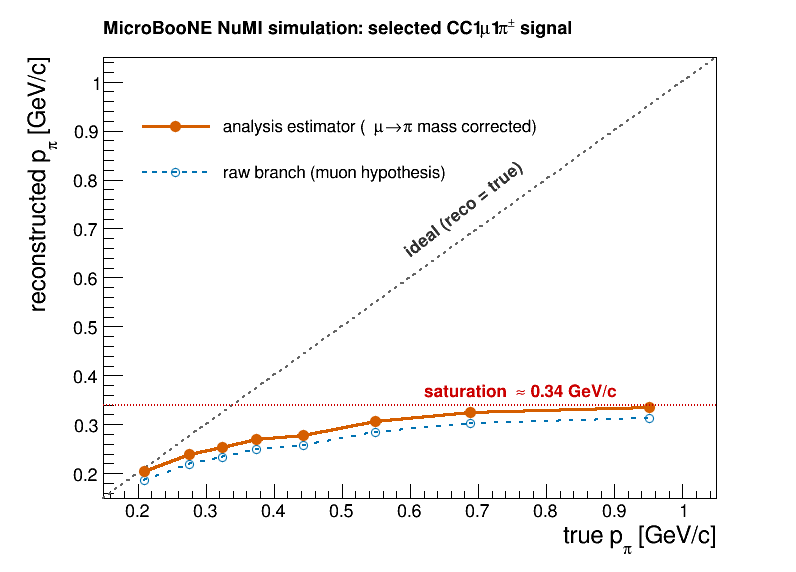
\includegraphics[width=0.72\textwidth]{ppi_saturation}
  \caption{Mean reconstructed against mean true pion momentum, selected signal. The
    analysis estimator (filled, $\mu\to\pi$ mass corrected) tracks truth at threshold but
    flattens out near $0.34$~GeV/$c$: a true $0.95$~GeV/$c$ pion reconstructs at the same
    place as a true $0.55$~GeV/$c$ one. The raw \texttt{candidate\_pion\_mom\_reco} branch
    (open) sits systematically below it by the uncorrected mass-hypothesis offset. The
    saturation is caused by hadronic interaction truncating the track range, and no
    range-based estimator can recover it.}
  \label{fig:ppi_sat}
\end{figure}

\paragraph{What that does to the response matrix.}
Migrating the five analysis bins with the corrected estimator gives a nearly
lower-triangular matrix: the diagonal fraction falls from $94.3\%$ in the first true bin
to $36.5$, $23.1$, $10.4$ and finally $6.2\%$ in the last. For the highest true bin
($p_\pi>0.55$~GeV/$c$) only $6.2\%$ of events are reconstructed in the corresponding reco
bin while $32.6\%$ fall all the way into the \emph{lowest} one. Every true bin above the
first therefore deposits most of its events into reco bin 1, which is exactly the
``pile-up into the first bin'' seen in \noteref{Fig.}{fig:response}.

\paragraph{How the BNB CC1$\pi^\pm$ analysis handles the same problem.}
The published BNB CC$1\pi^{\pm}$Xp analysis (internal note v0.91) faces an identical
estimator, it too takes ``the momentum of pion candidates from range'', and its
treatment is worth reproducing here, because it is the recipe this analysis followed.

That analysis does three things we do not. First, it defines a \emph{golden pion}: one
that comes to rest and leaves a Bragg peak, as opposed to one that scattered or interacted.
Second, it trains a dedicated \emph{golden-pion BDT} and applies it as an extra cut for
the pion-momentum differential cross section only, leaving the total and angular results on
the generic selection. The BDT separates golden from non-golden pions using track
``wiggliness'' (the standard deviation of the angular difference between directions of
adjacent points along the fitted track, so a direct handle on scattering), the number of
reconstructed descendant particles, the track--shower score, and the Bragg likelihood
ratio. The cost and benefit are quoted explicitly: efficiency falls from $20.3\%$ to
$9.5\%$ and purity is essentially unchanged ($51.9\to49.5\%$), but the golden fraction of
the selected signal rises from $36.3\%$ to $67.7\%$. They apply the same logic to the muon
momentum, restricting that cross section to contained muons ($8.4\%$ efficiency,
$56.1\%$ purity) so it uses range only.

Third, and most directly comparable, their binning is chosen against an explicit criterion:
each bin must hold at least 100 predicted MC events \emph{and} the diagonal element of the
smearing matrix must exceed $0.68$. The resulting pion-momentum edges are
$0.10, 0.16, 0.19, 0.22, 0.60$~GeV/$c$ with an overflow bin, fine structure only where
the estimator still tracks truth, then a single wide bin from $0.22$ to $0.60$ and
everything above $0.60$ in overflow.

Set against that criterion our binning does not survive: the diagonal fractions measured
above are $94.3, 36.5, 23.1, 10.4$ and $6.2\%$, so \emph{one} of five bins passes $0.68$
and the top three fail it by a wide margin. Our edges ($0.175$--$0.550$ in five bins, open
above) put four boundaries inside precisely the region where the reconstructed momentum has
saturated.

\paragraph{Consequences, and what would improve it.}
This is not a bias on the extracted cross section; the response matrix contains it and
the unfolding inverts it, but it is the reason the $p_\pi$ result leans harder on the
regularisation than any other observable. With $6\%$
diagonal strength in the top bin, the measurement above $\sim\!0.5$~GeV/$c$ is effectively
inferred from the response model rather than measured.

The BNB note therefore supplies a tested recipe, and \emph{all four} of its BDT inputs are
already available to us. The Bragg likelihood ratios (\texttt{trk\_bragg\_pion},
\texttt{\_mip}, \texttt{\_mu}, \texttt{\_p}) and the track--shower score are in the
ntuples; the multi-pion pion-ID BDT in this analysis already trains on exactly those,
and the descendant counts are \texttt{pfp\_trk\_daughters\_v} /
\texttt{pfp\_shr\_daughters\_v}. Wiggliness is there too, under a different name: the PeLEE
ntuples carry \texttt{trk\_avg\_deflection\_stdev\_v} (with companions
\texttt{\_mean\_v} and \texttt{\_separation\_mean\_v}), which is precisely the standard
deviation of the angular deflection between adjacent track points. It is fully populated
and is carried forward by \texttt{ProcessNTuples}.

\paragraph{Wiggliness works, but with the opposite sign to the naive expectation.}
Testing it directly on truth-matched charged pions in the Run-1 FHC overlay, calling a
pion ``golden-like'' when the mass-corrected range momentum recovers the true momentum to
within $20\%$, and ``interacting'' when it recovers less than $60\%$, gives a clear
separation, but golden pions are the \emph{wigglier} ones, by about a factor two in the
mean ($0.0048$ against $0.0027$). That is not a momentum artefact: it survives binning in
track length, with the ratio staying at $0.51$--$0.63$ from $5$~cm to $400$~cm.

The sign makes physical sense on reflection. A pion that stops travels its full range and
scatters violently through its final slow centimetres, so the deflection spread averaged
along the track is large. A pion that interacts hadronically is cut short while still fast
and never reaches that wiggly end, so its track is straighter. High wiggliness is thus a
signature of \emph{having stopped}, exactly the population for which a range-based
momentum is meaningful.

As a single cut it is already useful: on this sample the golden fraction is $39.9\%$ before
any cut, and requiring \texttt{trk\_avg\_deflection\_stdev\_v}$\,>0.001$ keeps $86.8\%$ of
golden pions while rejecting $48.8\%$ of interacting ones, lifting the golden fraction to
$53.0\%$. A tighter cut at $0.002$ gives $57.8\%$ efficiency and $55.7\%$ golden. For
reference the BNB's four-variable BDT reaches $67.7\%$ golden at roughly half the
generic-selection efficiency, so one variable recovers a good part of the gain and the
remaining three, all of which we have, should close much of the rest.

Three options follow from this, in increasing order of effort: rebin $p_\pi$ against
the BNB's own criterion (diagonal $>0.68$), which on the numbers above means one resolved
bin at threshold plus a wide open bin; add a golden-pion cut for the $p_\pi$ cross section
built from the variables already available, accepting the factor-two efficiency loss the
BNB analysis accepts; or reproduce their BDT in full. None changes the total or angular
results, which do not use this estimator. The first is the adopted scheme
(\S\ref{sec:ppi2bin_adopted}); the classifier was trained and tested and found not to
change the conclusion (\S\ref{sec:golden_bdt}).

\subsubsection*{Adopted response: a two-bin $p_\pi$ scheme}
\label{sec:ppi2bin_adopted}

The released binning is two bins,
$[0.175, 0.205]$~GeV/$c$ and everything above, which raises the migration diagonals from
$96/35/21/10/6\%$ (full analysis sample; $94.3/36.5/23.1/10.4/6.2\%$ on Run~1 alone,
Table~\ref{tab:ppi_sat}) to $\mathbf{91/76\%}$, clearing the $68\%$ criterion in \emph{both} bins.
(These are measured on the analysis sample; the golden-pion study of
Sec.~\ref{sec:golden_bdt} uses a looser track sample whose diagonals are lower, and the two
sets are not interchangeable.)

The boundary is not a free choice dressed up as an optimisation. The worst diagonal is
always the upper bin and it falls monotonically as the boundary rises, so the binding
constraint is the \emph{width} of the first bin rather than the diagonal itself:

\begin{center}\small
\begin{tabular}{lccc}
\toprule
boundary & first-bin width & diagonal, bin 1 & diagonal, bin 2 \\\midrule
$0.185$ & $10$~MeV/$c$ & $79.7\%$ & $85.4\%$ \\
$0.195$ & $20$~MeV/$c$ & $88.8\%$ & $80.0\%$ \\
$0.200$ & $25$~MeV/$c$ & $90.4\%$ & $77.7\%$ \\
\textbf{0.205} & \textbf{30~MeV/}$\mathbf{c}$ & $\mathbf{91.0\%}$ & $\mathbf{75.5\%}$ \\
$0.220$ & $45$~MeV/$c$ & $93.3\%$ & $69.1\%$ \\
$0.250$ & $75$~MeV/$c$ & $95.6\%$ & $56.1\%$ \\
$0.300$ & $125$~MeV/$c$ & $96.3\%$ & $39.0\%$ \\
\bottomrule
\end{tabular}
\end{center}

\noindent Both bins clear the criterion anywhere between roughly $0.19$ and $0.22$, so the
choice within that window is governed by bin width rather than by the criterion. $0.205$ is
the narrowest first bin with precedent: $30$~MeV/$c$ matches the narrowest bin used in the
BNB CC$1\pi$ analysis. Going narrower trades first-bin diagonal for upper-bin diagonal and
at $10$~MeV/$c$ the first bin itself falls to $80\%$ on only $325$ events, which is not a
useful cross-section bin; going wider, $0.220$ still passes but leaves the upper bin at
$69\%$, with no margin. An exhaustive scan over all edge sets
(\texttt{macros/ppi\_binning\_scan.C}) returns $0.205$ as the best first boundary for every
number of bins tried, and for the proton-tagged selection as well.

A three-bin variant was built and measured before being discarded. The best achievable
(same $30$~MeV/$c$ minimum width, edges $0.205$ and $0.265$) is $91/51/52\%$, against
$91/76\%$ for two bins: the third bin costs $25$ points on the worst bin and drops it well
below the criterion. Two $30$~MeV/$c$ bins followed by an open bin
($0.205$, $0.235$) is worse still at $91/39/62\%$, and note that it degrades the
\emph{upper} bin too, from $76\%$ to $62\%$: narrowing the top bin's reco range pushes
genuinely high-momentum events out of their own bin. Four bins reach only $91/39/39/42\%$. Above $\sim\!0.25$~GeV/$c$ the reconstructed
momentum barely varies, so a second boundary there separates almost nothing and merely
divides one poorly-measured region into two equally poor halves. The same ordering holds
under a golden-pion cut ($67/52/46\%$), so it is not an artefact of the selection.

\paragraph{Closure.} The two-bin scheme is carried through the full chain, universe
construction, Wiener--SVD unfolding and systematics, and closes in all three configurations
(Table~\ref{tab:ppi2bin}); a five-bin extraction on the same sample closes too, at
$\chi^2\approx2/5$, which is the point: closure cannot expose a response that carries no
shape information, only the migration criterion can.

\begin{table}[htbp]\centering
\caption{Two-bin $p_\pi$ result for all three beam configurations, $d\sigma/dp_\pi$ in
  $10^{-38}$~cm$^2$/(GeV/$c$)/Ar. Bin~1 is $[0.175,0.205]$~GeV/$c$, bin~2 everything above.
  All curves are $A_C$-smeared, so they live in the same space as the measurement.
  Generated from the 2026-09-06 release (\texttt{report/tools/ppi2bin\_tables.py}: closure sidecars and
  \texttt{curves\_incl\_*\_ppi2bin.tsv}); the uncertainty row is the total.}
\label{tab:ppi2bin}
\begin{tabular}{lccc|ccc|ccc}
\toprule
 & \multicolumn{3}{c|}{FHC} & \multicolumn{3}{c|}{RHC} & \multicolumn{3}{c}{Combined} \\
 & bin 1 & bin 2 & $\sigma_\mathrm{int}$ & bin 1 & bin 2 & $\sigma_\mathrm{int}$
 & bin 1 & bin 2 & $\sigma_\mathrm{int}$ \\\midrule
unfolded data & $1.96$ & $0.96$ & $0.822$ & $1.79$ & $0.87$ & $0.748$ & $2.06$ & $0.90$ & $0.775$ \\
uncertainty   & $\pm1.36$ & $\pm0.37$ &  & $\pm1.12$ & $\pm0.34$ &  & $\pm1.26$ & $\pm0.34$ &  \\
$A_C$ truth   & $2.34$ & $0.95$ &  & $1.71$ & $0.89$ &  & $2.17$ & $0.90$ &  \\
uB tune       & $2.29$ & $0.93$ &  & $1.72$ & $0.88$ &  & $2.15$ & $0.89$ &  \\\midrule
GENIE & $1.82$ & $0.75$ &  & $1.29$ & $0.63$ &  & $1.67$ & $0.67$ &  \\
GiBUU & $3.28$ & $0.94$ &  & $2.27$ & $0.82$ &  & $3.03$ & $0.85$ &  \\
NEUT  & $3.09$ & $1.18$ &  & $2.24$ & $1.02$ &  & $2.87$ & $1.07$ &  \\
NuWro & $2.98$ & $1.12$ &  & $2.11$ & $0.96$ &  & $2.74$ & $1.01$ &  \\
\midrule
$\chi^2/\mathrm{ndf}$ & \multicolumn{3}{c|}{$0.11/2$ ($p=0.95$)} & \multicolumn{3}{c|}{$0.01/2$ ($p=0.99$)} & \multicolumn{3}{c}{$0.01/2$ ($p=1.00$)} \\
\bottomrule
\end{tabular}
\end{table}

\begin{figure}[htbp]\centering
  \begin{subfigure}[b]{0.32\textwidth}
    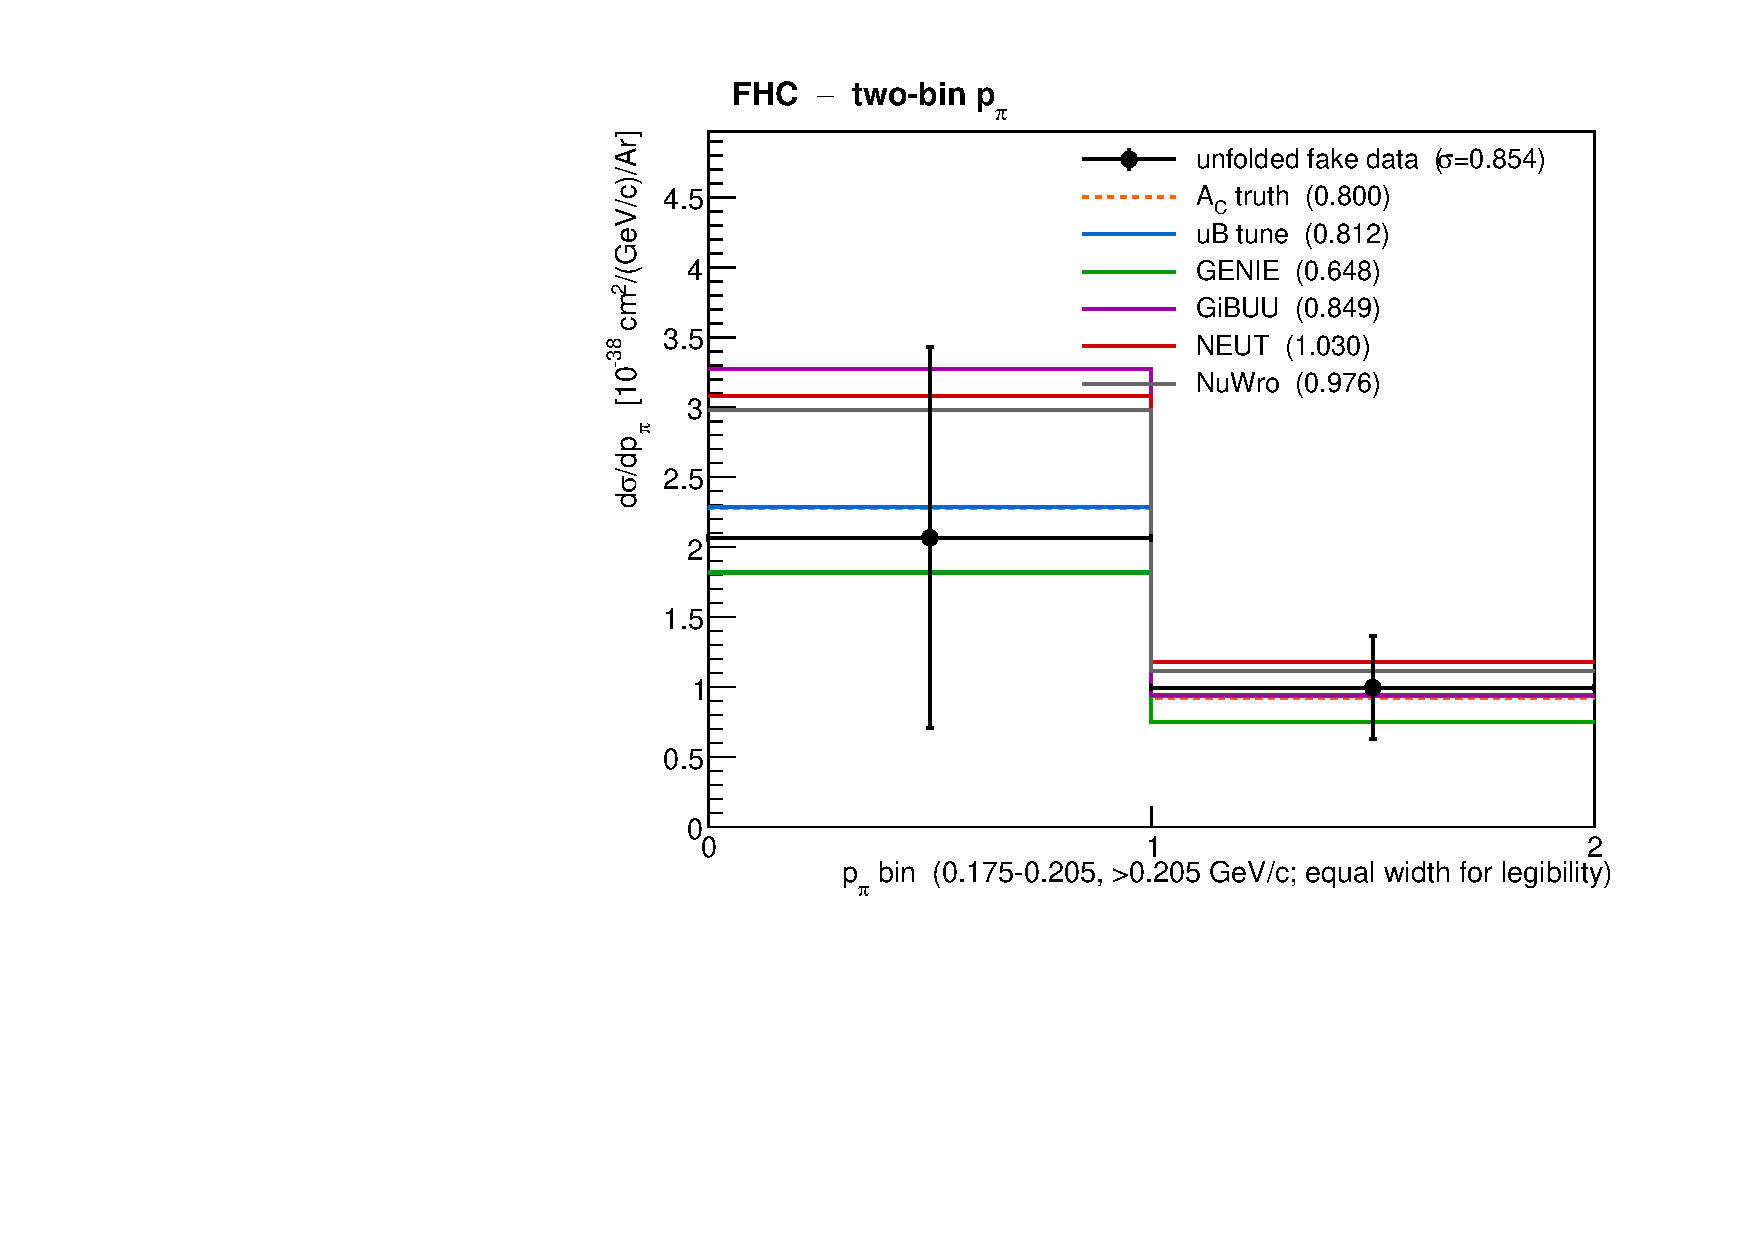
\includegraphics[width=\textwidth]{ppi2bin_xsec_FHC}\caption{FHC}
  \end{subfigure}\hfill
  \begin{subfigure}[b]{0.32\textwidth}
    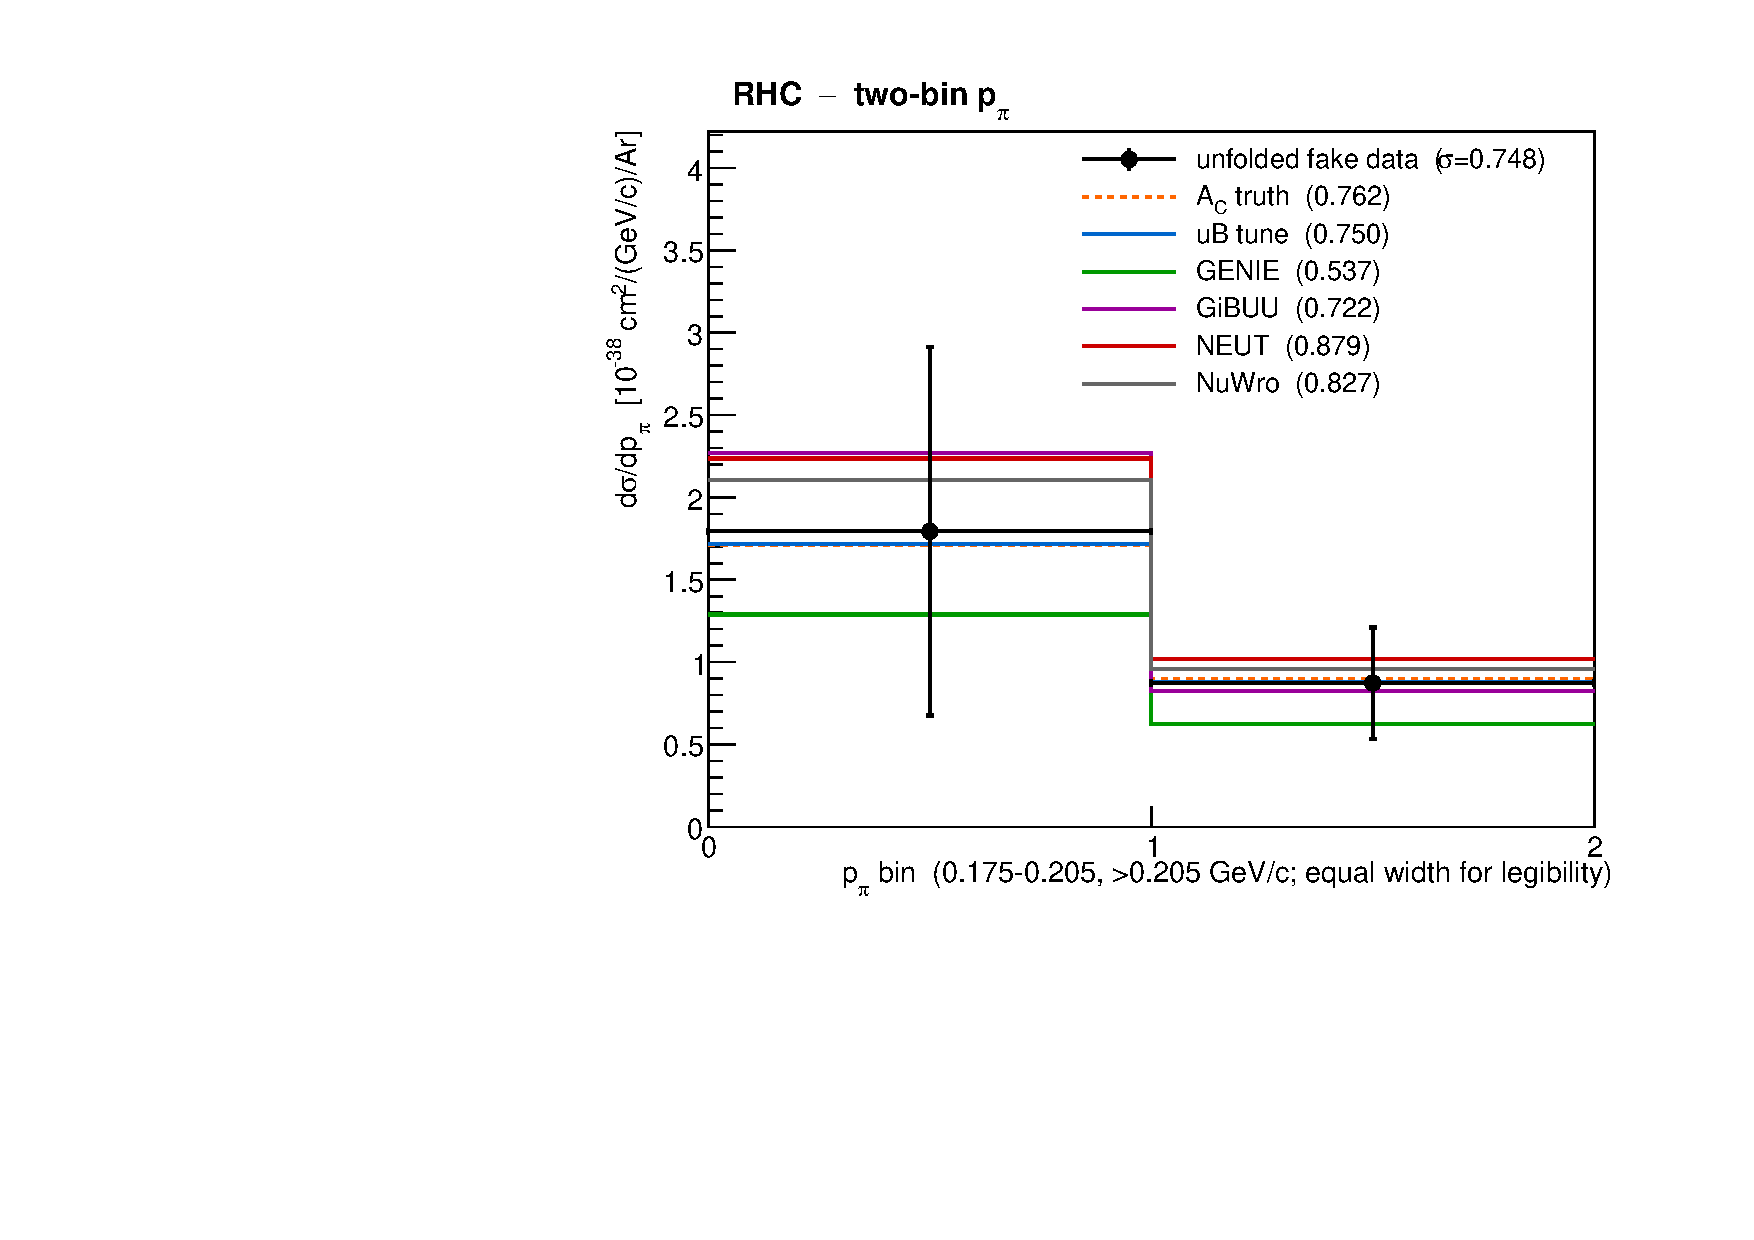
\includegraphics[width=\textwidth]{ppi2bin_xsec_RHC}\caption{RHC}
  \end{subfigure}\hfill
  \begin{subfigure}[b]{0.32\textwidth}
    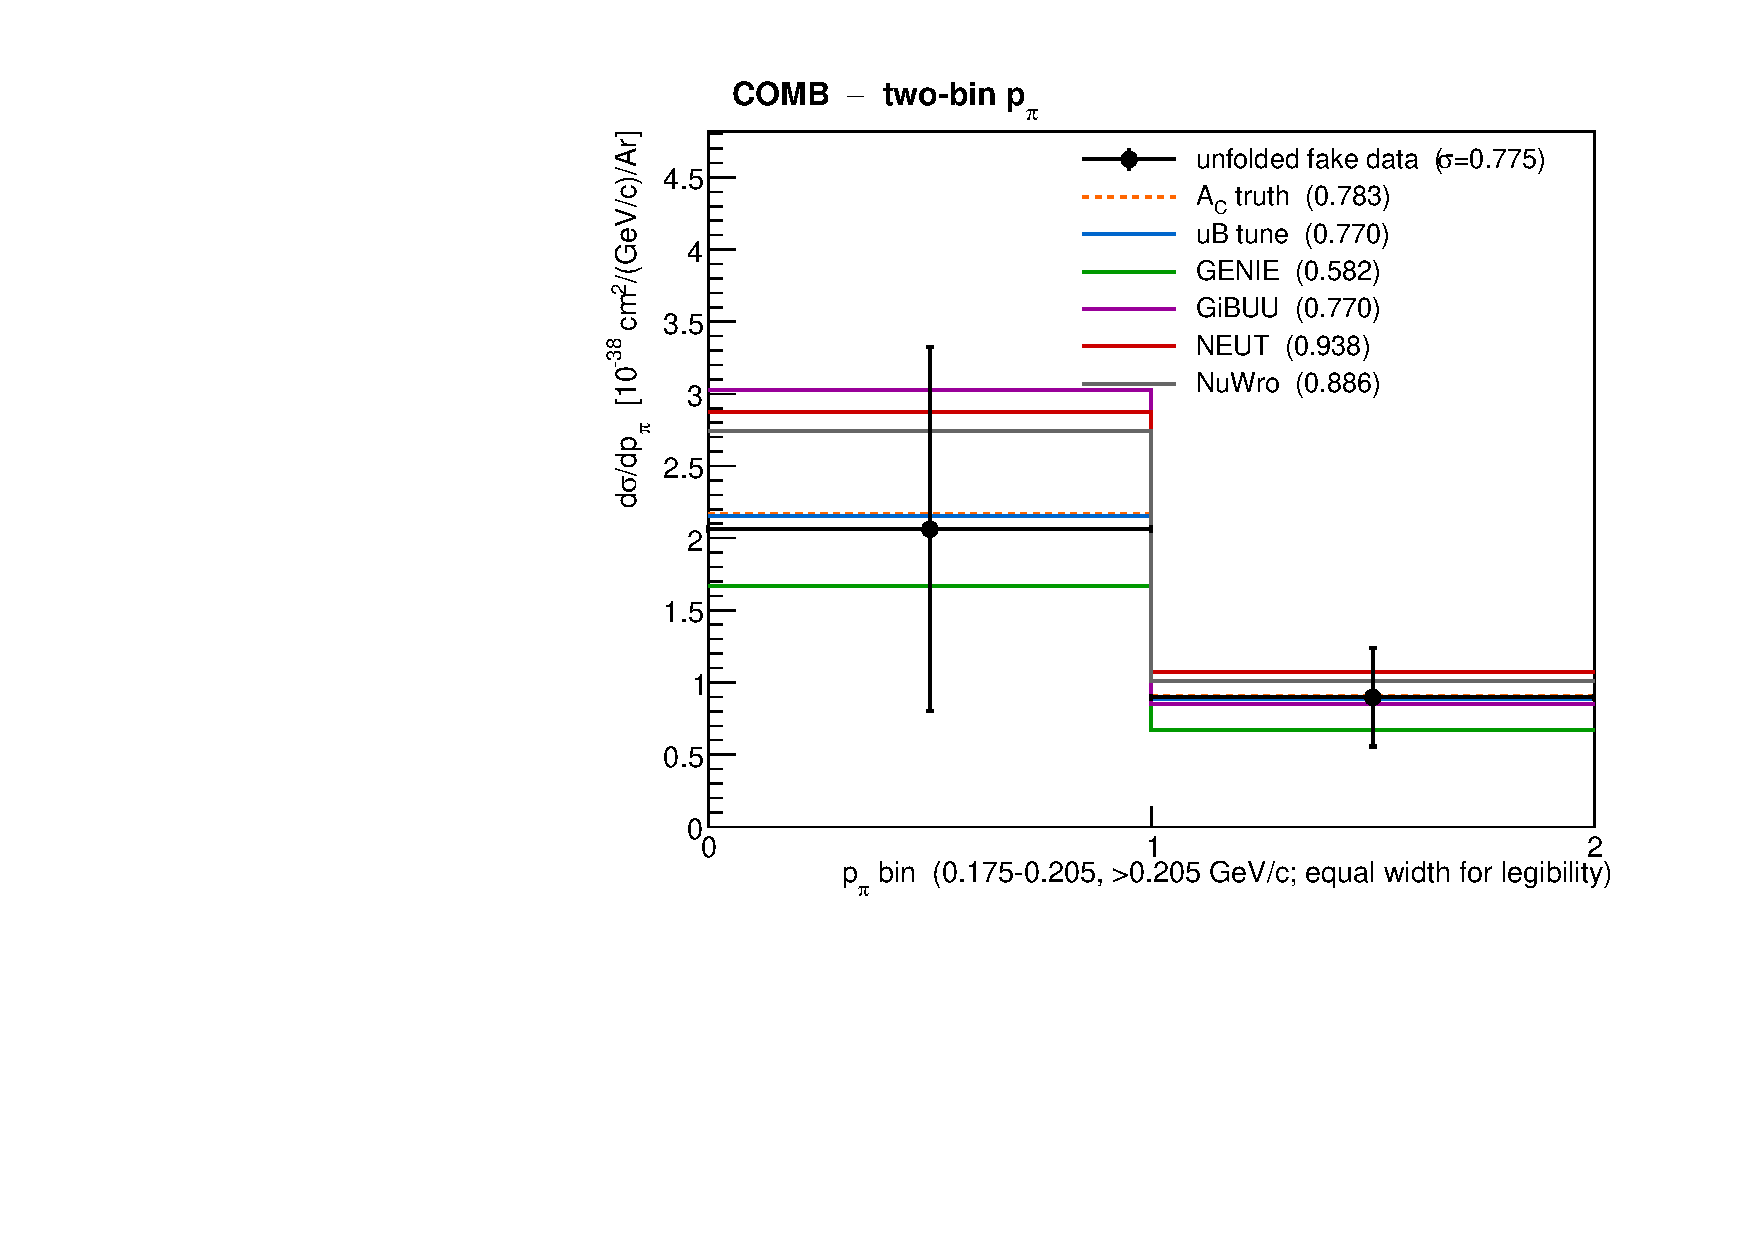
\includegraphics[width=\textwidth]{ppi2bin_xsec_COMB}\caption{Combined}
  \end{subfigure}
  \caption{The two-bin $p_\pi$ cross section, the graphical form of
    Tab.~\ref{tab:ppi2bin}. Unfolded fake data (points, with the full systematic
    uncertainty) against the $A_C$-smeared truth, the uB tune and the four generators; every
    curve is $A_C$-smeared, so all of them live in the same space as the measurement.
    \textbf{The two bins are drawn with equal width for legibility}: they are $0.030$ and
    $0.795$~GeV/$c$ wide, so to scale the first would occupy $4\%$ of the axis. Area on
    these panels is therefore not proportional to cross section, and the integrated
    $\sigma$ is printed on each panel instead. The generators bracket the data in every bin
    of every configuration; GENIE is generally the lowest prediction and NEUT and GiBUU
    the highest, and which generator is closest changes from bin to bin.}
  \label{fig:ppi2bin_xsec}
\end{figure}

\noindent On the current release all three configurations close, with $\chi^2$ of $0.11$,
$0.015$ and $0.01$ on two bins (the RHC value rounds either way in the note's tables) and
unfolded-to-truth integral ratios of $0.997$, $0.981$ and $0.989$ (width-weighted
unfolded over $A_C$-smeared truth from the released curves,
\texttt{curves\_incl\_*\_ppi2bin.tsv}; the $\chi^2$ from Tables~\ref{N-tab:fhc}--\ref{N-tab:comb}
of the analysis note). The
four generators bracket the data in both bins of every configuration, NEUT and GiBUU
highest and GENIE lowest, the same ordering as in the other observables; the released
$A_C$ for FHC is $\left(\begin{smallmatrix} 0.53 & 0.01 \\ -0.51 & 0.87 \end{smallmatrix}\right)$
(\texttt{A\_C\_incl\_FHC5\_ppi2bin.tsv}), whose off-diagonal element is the reminder that
the two bins are not independent after merging. The total fractional uncertainty is
$50\%$ (FHC), the largest of the inclusive observables, because the two bins each carry a
large share of the flux normalisation with little statistical averaging.
Figure~\ref{fig:ppi2bin_AC} shows $A_C$ for all three configurations (release 2026-09-06).
RHC regularises a little harder than FHC in the first bin (diagonal $0.38$ against $0.53$,
off-diagonal $-0.37$ against $-0.51$), and the combined extraction borrows the most
(diagonal $0.53$, off-diagonal $-0.58$); the second-bin diagonals are $0.87$--$0.88$ in all
three. Despite the different conditioning the three extractions close in normalisation
within $2\%$ (the ratios $0.997$, $0.981$ and $0.989$ above), so there is no common
normalisation offset associated with how hard $A_C$ smears.

\begin{figure}[htbp]\centering
  \begin{subfigure}[b]{0.32\textwidth}
    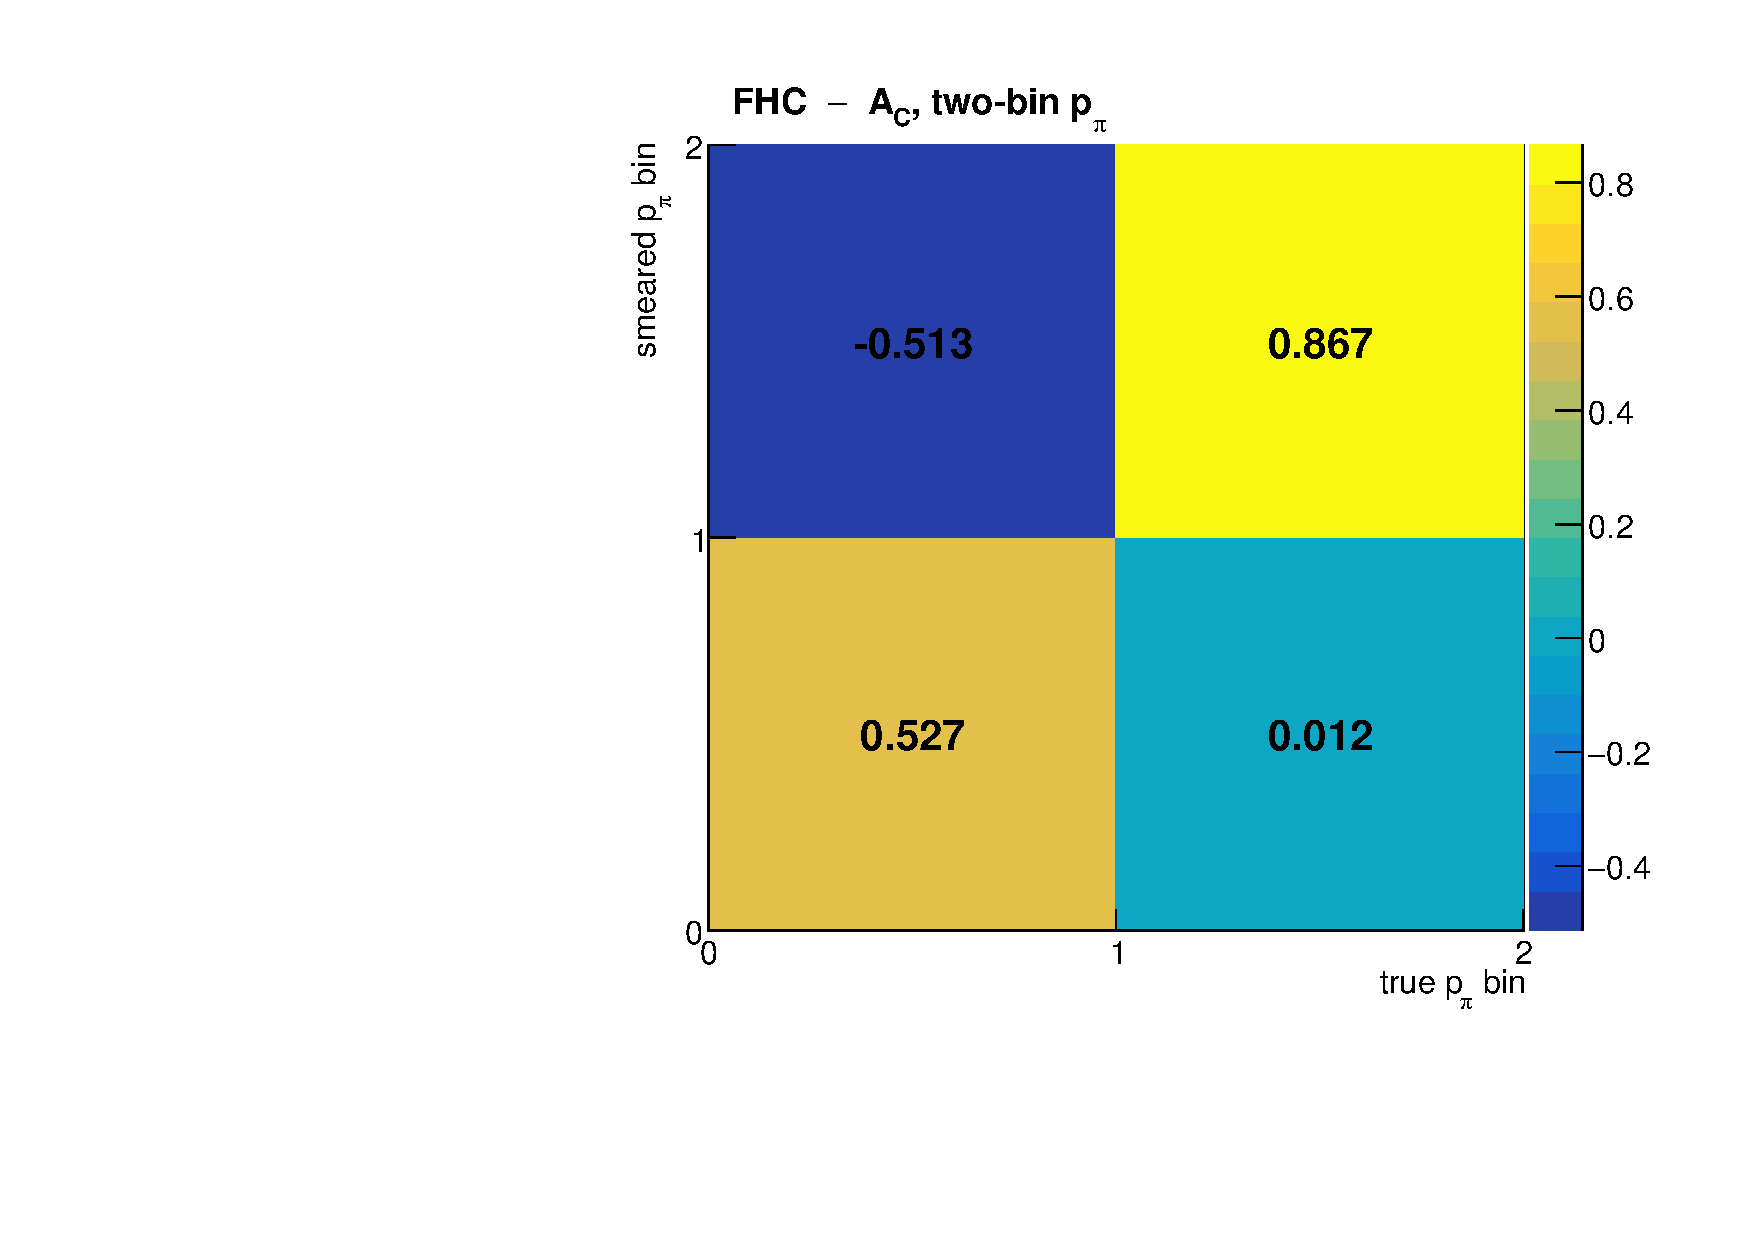
\includegraphics[width=\textwidth]{ppi2bin_AC_FHC}\caption{FHC}
  \end{subfigure}\hfill
  \begin{subfigure}[b]{0.32\textwidth}
    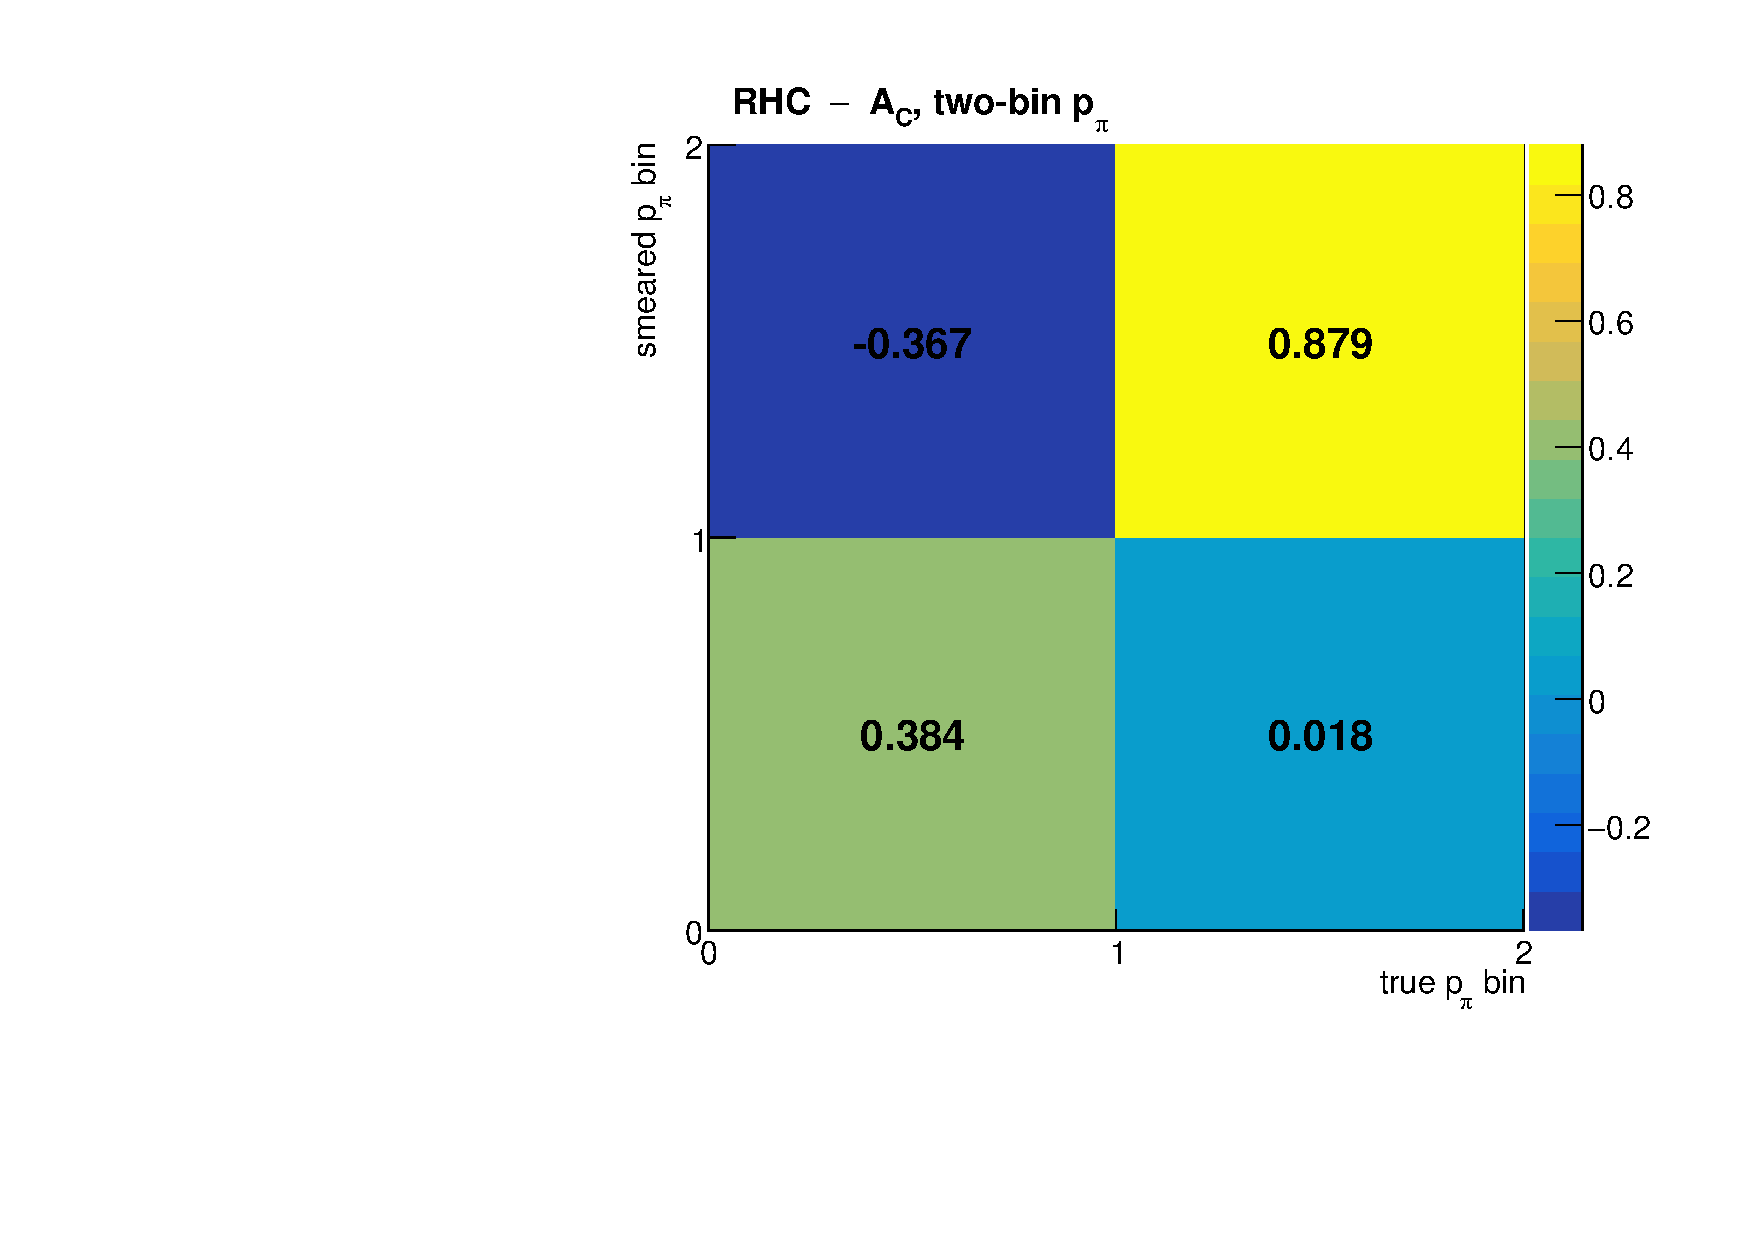
\includegraphics[width=\textwidth]{ppi2bin_AC_RHC}\caption{RHC}
  \end{subfigure}\hfill
  \begin{subfigure}[b]{0.32\textwidth}
    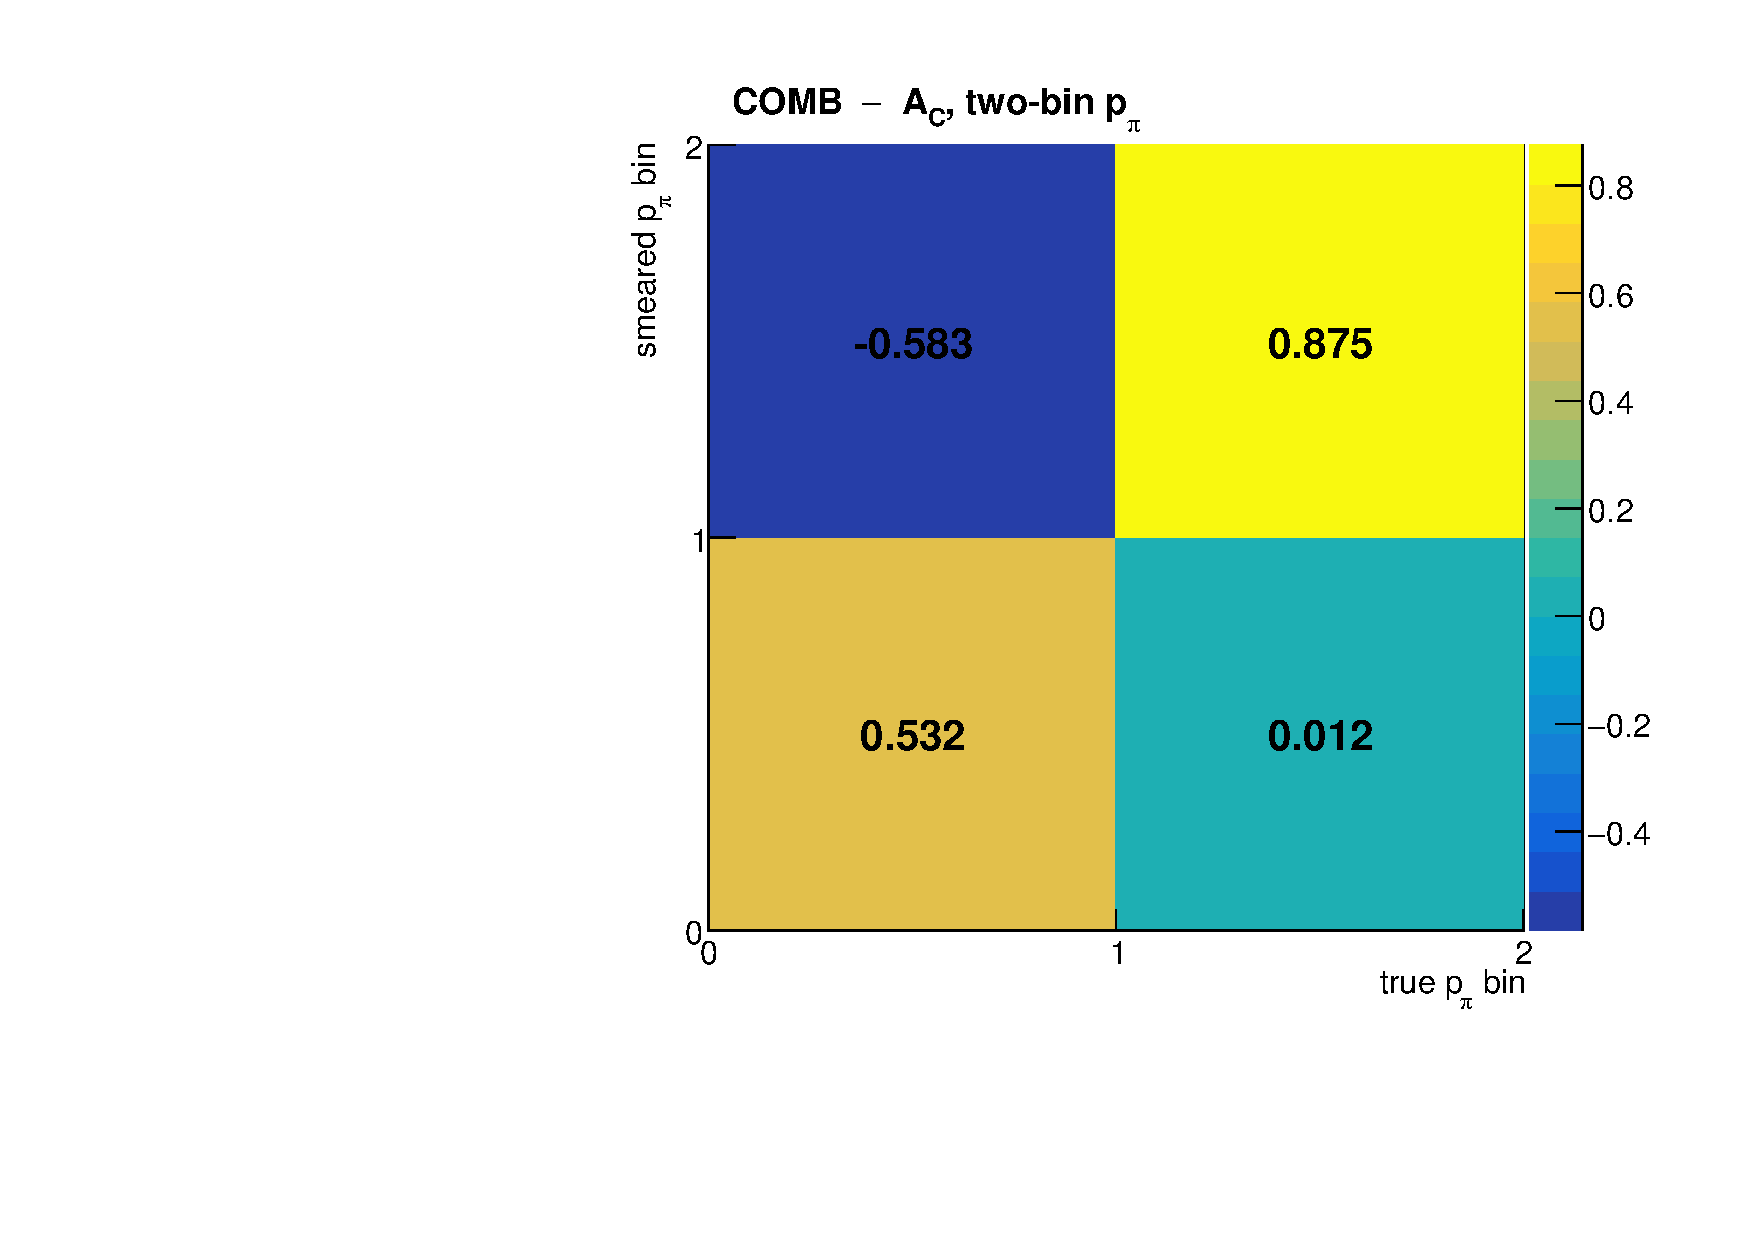
\includegraphics[width=\textwidth]{ppi2bin_AC_COMB}\caption{Combined}
  \end{subfigure}
  \caption{The additional-smearing matrix $A_C$ for the two-bin $p_\pi$ scheme, in the
    convention $\hat{x}_i = \sum_j (A_C)_{ij}\, t_j$ so that a column is a true bin and a
    row is the smeared bin it feeds. $A_C$ is not normalisation-preserving, so its rows do
    not sum to unity. The negative entry (true bin~1 feeding smeared bin~2, drawn top-left
    since the smeared axis runs upward) is the regularisation borrowing between the two
    bins; it is why the truth curves in
    Fig.~\ref{fig:ppi2bin_xsec} must be $A_C$-smeared before being compared with the
    measurement rather than plotted raw.}
  \label{fig:ppi2bin_AC}
\end{figure}

At $91/76\%$ both bins clear the $68\%$ criterion, so the two-bin scheme makes the inclusive
$p_\pi$ result usable on the standard test rather than merely honest about its limitations.
It remains a coarse measurement: two bins cannot resolve a shape, and above
$\sim\!0.34$~GeV/$c$ the reconstructed momentum saturates, so the upper bin is an integral
over a wide range rather than a differential point. What the scheme buys is a result whose
response is defensible, not a competitive shape measurement.

\subsubsection*{A golden-pion classifier was trained and tested: it works, and it is not enough}
\label{sec:golden_bdt}

Following the BNB recipe, a golden-pion BDT was trained and evaluated
(\texttt{macros/golden\_pion\_train.C}, \texttt{macros/golden\_pion\_compare.C}). The truth
label is \texttt{mc\_end\_p} $<0.01$~GeV/$c$, the pion ranged out, joined to
reconstruction by matching \texttt{backtracked\_p} to \texttt{mc\_p}, which pairs $100\%$ of
candidate tracks with no ambiguity. The inputs are the three deflection variables, the four
Bragg likelihood ratios, the track--shower score and the descendant count. Training used
$126\,518$ labelled tracks from Runs 1, 2 and 4; the split is by \emph{run}, so all numbers
below are on Run 2, which the classifier never saw.

\paragraph{As a classifier it reproduces the BNB benchmark.} ROC integral $0.758$. At
$44.8\%$ efficiency it lifts the golden fraction from $43.1\%$ to $64.9\%$, against the BNB's
$36.3\to67.7\%$ at roughly $47\%$ efficiency. The variable ranking is dominated by the
deflection variables (\texttt{wmean}, then \texttt{wstd}), with the Bragg ratios contributing
essentially nothing, worth noting, since Bragg was expected to carry the stopping
signature.

\paragraph{But it does not fix the binning, and cannot.} Table~\ref{tab:golden_compare}
gives the migration diagonal in the five analysis bins as the cut is tightened. The first bin
is already fine and stays fine; no other bin reaches $0.68$ at any working point, even at
$15\%$ efficiency.

\begin{table}[htbp]\centering
\caption{Golden-pion BDT: efficiency, achieved golden fraction, and the $p_\pi$ migration
  diagonal per true bin, on the held-out run. The BNB criterion for a usable bin is a
  diagonal above $0.68$.}
\label{tab:golden_compare}
\begin{tabular}{lccccccc}
\toprule
BDT cut & eff. & golden frac. & b1 & b2 & b3 & b4 & b5 \\\midrule
none      & $100\%$  & $43.1\%$ & 99.2 & 23.7 & 13.2 & 6.4 & 5.5 \\
$>-0.05$  & $57.0\%$ & $58.1\%$ & 99.1 & 29.4 & 19.7 & 11.2 & 7.1 \\
$>0.00$   & $44.8\%$ & $64.9\%$ & 99.1 & 33.1 & 24.5 & 15.4 & 9.1 \\
$>+0.10$  & $24.6\%$ & $79.4\%$ & 99.1 & 42.9 & 36.8 & 29.3 & 15.7 \\
$>+0.15$  & $15.2\%$ & $84.5\%$ & 99.2 & 46.9 & 42.2 & 36.1 & 19.5 \\\midrule
\multicolumn{3}{l}{\emph{perfect (truth) golden selection}} & 98.9 & 36.1 & 24.1 & 14.2 & 8.9 \\
\bottomrule
\end{tabular}
\end{table}

\paragraph{These diagonals are measured on a different sample from the analysis ones, and
the two must not be mixed.} The table above is built on the labelled \emph{track} sample:
every truth-matched pion track passing loose quality requirements (purity $>0.5$, track
score $>0.5$, length $>5$~cm), from events of any topology, $126\,518$ tracks in total. The
migration diagonals quoted elsewhere in this note, $96/35/21/10/6\%$ for five bins and
$91/76\%$ for two, are measured on the \emph{analysis} sample: events passing the full
CC$1\mu1\pi^\pm$ selection and satisfying the signal definition, about $10\,700$ per beam
mode. The analysis sample has the better response, because the selection removes exactly the
events whose pion is poorly reconstructed. On the track sample the same five-bin scheme reads
$99/24/13/6/6\%$ and the two-bin scheme $98/62\%$.

Those track-sample figures are not the analysis response, and the $62\%$ must not be
read as the inclusive $p_\pi$ measurement failing the usable-bin criterion. It does not: on
the analysis sample the upper bin sits at
$76\%$. The numbers in this table are correct for what they measure, and the conclusions
drawn \emph{within} it, which compare rows of the same sample, are unaffected.

The last row is the decisive one, and it must be read against the \emph{efficiency} column
rather than against the tightest cut. Perfect truth-level golden selection keeps $43.1\%$ of
tracks and gives $36.1, 24.1, 14.2, 8.9\%$ in bins 2--5; the classifier at the matching
$44.8\%$ efficiency gives $33.1, 24.5, 15.4, 9.1\%$. They agree bin by bin. The classifier
is therefore already performing as well as perfect knowledge of which pions stopped, and no
better classifier exists to be built.

\paragraph{Multiple Coulomb scattering was tried as a pion momentum estimator, and as a
classifier input.} Range saturates because the pion interacts before stopping, which
truncates the track. Multiple-Coulomb-scattering (MCS) momentum is inferred from the
scattering along whatever track exists and is not truncated by an interaction, so it is the
natural candidate to replace range. The CC0$\pi$ analysis uses exactly this pairing, range
for contained tracks and MCS for exiting ones. Measured on $122\,878$ truth-matched pion
tracks (\texttt{trk\_mcs\_muon\_mom\_v}, filled for $99.9\%$ of them):

\begin{center}\small
\begin{tabular}{lcccccc}
\toprule
true $p_\pi$ [GeV/$c$] & $\langle$len$\rangle$ & $\langle$range/true$\rangle$ & RMS
 & $\langle$MCS/true$\rangle$ & RMS \\\midrule
$0.175$--$0.250$ & $25$~cm & $0.834$ & $0.16$ & $4.335$ & $14.1$ \\
$0.320$--$0.420$ & $46$~cm & $0.629$ & $0.23$ & $2.438$ & $7.2$ \\
$0.550$--$0.800$ & $71$~cm & $0.446$ & $0.18$ & $1.423$ & $3.5$ \\
$0.800$--$1.500$ & $84$~cm & $\mathbf{0.319}$ & $0.16$ & $\mathbf{1.011}$ & $2.1$ \\
\bottomrule
\end{tabular}
\end{center}

\noindent The trade is stark. In the top bin range is biased to $0.319$, which is the
saturation, while MCS is essentially unbiased at $1.011$; but MCS carries a $210\%$ RMS
there and $1400\%$ in the lowest bin. It is unusable as a per-event estimator. The reason is
structural and explains why the CC0$\pi$ recipe does not transfer: they apply MCS to
\emph{exiting} tracks, which are long by construction, whereas our problematic pions are
contained but interacting, $25$--$84$~cm long, and MCS needs of order a metre.

The same note uses the \emph{disagreement} between the two estimators as a track-quality BDT
input rather than as an estimator. That is well motivated here: a pion that interacts has a
truncated range but an untruncated MCS, so the fractional difference
$(p_\mathrm{range}-p_\mathrm{MCS})/p_\mathrm{range}$ should flag precisely the events that
break the response. Adding it to the golden-pion classifier, it ranks \emph{second of ten}
in importance, behind only the mean deflection. It nonetheless changes nothing:

\begin{center}\small
\begin{tabular}{lcc}
\toprule
classifier inputs & ROC integral & diagonals at $\sim\!44\%$ efficiency \\\midrule
baseline (nine variables) & $0.758$ & $99.1 / 33.1 / 24.5 / 15.4 / 9.1$ \\
$+$ range$-$MCS difference & $0.757$ & $99.0 / 34.8 / 24.8 / 14.8 / 9.1$ \\
\bottomrule
\end{tabular}
\end{center}

\noindent The interpretation is that the new variable is highly informative but not
\emph{additionally} informative: it is strongly correlated with the deflection variables
already present, since both measure whether the track scattered heavily and ended abruptly.
High importance rank with unchanged ROC is the signature of a redundant input. This is an
independent confirmation of the ceiling argument above: the classifier already extracts what
golden-ness has to offer, and the limit is the physics of the label rather than the quality
of the classifier.

One tempting variant was deliberately not pursued. Retraining on the label ``range is
accurate'', $|p_\mathrm{corr}/p_\mathrm{true}-1|<0.2$, would target the quantity we actually
care about and would certainly raise the diagonals. It would also be selecting on the answer:
keeping events where the estimator happens to be right sculpts the response by construction
and inflates the diagonal without measuring anything, the same trap documented for the tight
BDT working point above. The golden label is used precisely because it is a physical property
of the pion, independent of how well it was reconstructed.


\paragraph{A caveat on the tighter working points.} The $>0.15$ row looks better than
perfect truth selection ($46.9, 42.2, 36.1, 19.5\%$), which is impossible for an honest
classifier and is worth understanding rather than quoting. It arises because a hard cut on
the classifier preferentially keeps \emph{long} tracks: inside the top true bin, the surviving
tracks have a mean length of $120.8$~cm against $78.2$~cm for all pions, and a mean
reconstructed momentum of $0.406$ against $0.307$~GeV/$c$. The cut is thus partly a cut on
the reconstructed momentum itself, which raises the diagonal by construction while sculpting
the spectrum. The apparent gain is circular and the tight working points should not be used.
This is the same failure mode anticipated for track length as a direct input; it enters here
through the deflection variables, which correlate with length, even though length itself was
excluded from training.

\paragraph{Why, and what is left.} Golden pions still reconstruct at
$\langle p^{\rm corr}/p^{\rm true}\rangle = 0.73$ on this sample. Interaction is therefore
not the only problem: the momentum conversion is itself biased. A single flat rescaling does
\emph{not} repair it, applying the best global factor drops the first bin from $98.9$ to
$49.1\%$ and leaves $0/5$ bins passing; because the bias is momentum-dependent, exactly as
the saturation curve of Figure~\ref{fig:ppi_sat} shows.

Coarser binning helps but does not rescue it either. Collapsing to two bins ($0.175$,
$0.230$, $\infty$) gives $98.7$ and $58.3\%$ with perfect golden selection: better, still
short of $0.68$. Only a single bin; that is, no differential measurement at all,
trivially passes.

\paragraph{Conclusion.} The comparison is worth stating plainly rather than filing as a
partial success. The classifier does what it was built to do and matches the published
benchmark, but the $p_\pi$ differential measurement above $\sim\!0.23$~GeV/$c$ cannot be made
to meet the BNB's own binning criterion with a range-based estimator, with or without a
golden-pion cut. The BNB analysis passes that criterion because its resolved bins
($0.10$--$0.16$, $0.16$--$0.19$, $0.19$--$0.22$) all sit \emph{below} our $0.175$~GeV/$c$
threshold, in the region where range still tracks momentum; above $0.22$ it uses a single
wide bin and an overflow. The realistic options for this analysis are therefore to lower the
pion threshold toward $0.10$~GeV/$c$ and resolve the region where the estimator works, to
adopt a two-bin-plus-overflow $p_\pi$ result and say so, or to replace the range-based
estimator altogether. The golden-pion BDT is a useful ingredient in any of those, but it is
not by itself the fix.

\medskip\noindent\fbox{\parbox{0.97\linewidth}{\textbf{Scope of this conclusion.} The
failure described in this subsection concerns attempts to recover a finer multi-bin $p_\pi$
spectrum, and its numbers are for the loose truth-matched track sample. It does not
invalidate the adopted two-bin analysis-sample result (\S\ref{sec:ppi2bin_adopted},
Table~\ref{tab:ppi2bin}), whose migration diagonals are $91\%$ and $76\%$.}}

\paragraph{Scope of $p_\pi$.} Both candidate routes to a finer $p_\pi$ measurement were
tried; as the preceding subsection and the following paragraph show, the golden-pion
classifier does not repair the response even at perfect truth-level selection, whereas the
proton tag does not change the response appreciably either way. At the two-bin scheme the
inclusive selection already satisfies the binning criterion, so $p_\pi$ need not be withdrawn
from it; what it cannot support is the five-bin \emph{shape} measurement originally planned.
The other inclusive observables are unaffected: the angular variables and $p_\mu$ retain
their shape information, and the total cross section does not use this estimator at all.

\paragraph{The proton-tagged route.} The other candidate route to a sharper $p_\pi$
response is the proton tag. It has been measured for FHC, RHC and the combined exposure:
at the same two-bin edges the proton-tagged response is indistinguishable from the
inclusive one, marginally worse rather than better. Applying the same migration-diagonal
test gives

\begin{center}\small
\begin{tabular}{llccc c}
\toprule
selection & config. & $N_\mathrm{sig}$ bin 1 & bin 1 $[0.175,0.205]$
 & bin 2 ($>0.205$) & both $>0.68$? \\\midrule
inclusive \texttt{CC1mu1piXp} & FHC & $1056$ & $91.0\%$ & $75.5\%$ & yes \\\midrule
\textbf{proton-tagged} & FHC & $469$ & $\mathbf{88.9\%}$ & $\mathbf{74.2\%}$ & \textbf{yes} \\
\texttt{CC1mu1pi1p} & RHC & $621$ & $\mathbf{89.4\%}$ & $\mathbf{75.1\%}$ & \textbf{yes} \\
 & comb. & $1090$ & $\mathbf{89.2\%}$ & $\mathbf{74.7\%}$ & \textbf{yes} \\
\bottomrule
\end{tabular}
\end{center}

\noindent measured on the \texttt{numuMC} overlays named in the corresponding
\texttt{file\_properties} lists, selected signal, with the reconstructed momentum
mass-corrected exactly as the bin config does it. All four rows clear the criterion in both
bins, and the proton-tagged values sit about two points \emph{below} the inclusive ones
rather than above them. The three proton-tagged configurations agree to better than a
percentage point, so the response is a property of the selection rather than of a particular
exposure, but the proton tag does not improve it.

That is the expected result. The pion-momentum response is set by whether the pion ranges out or interacts
hadronically before stopping, which is a property of the pion's own passage through the
argon. Requiring a reconstructed proton at the vertex changes the event sample, the purity
and the efficiency, but it does not change what happens to the pion downstream, so there is
no mechanism by which it would sharpen the momentum response, and the measurement says so
directly.

The consequence is that the proton-tagged $p_\pi$ measurement stands on its own merits, as
the pion-momentum cross section of an exclusive final state that also yields $W$ and TKI, and
not as a repair of the inclusive one. The inclusive $p_\pi$ at two bins is equally
defensible on the response test.

\begin{table}[htbp]\centering
\caption{Two-bin $p_\pi$ on the proton-tagged \texttt{CC1mu1pi1p} selection, all three beam
  configurations. $d\sigma/dp_\pi$ in $10^{-38}$~cm$^2$/(GeV/$c$)/Ar; bin~1 is
  $[0.175,0.205]$~GeV/$c$, bin~2 everything above. All curves are $A_C$-smeared. The
  proton-tagged \texttt{xsec} configs declare only the tune and the fake data, so no
  generator rows appear. Regenerated from the 2026-09-06 release
  (\texttt{report/tools/ppi2bin\_tables.py}); the uncertainty row is the total.}
\label{tab:ppi2bin_1p}
\begin{tabular}{lcc|cc|cc}
\toprule
 & \multicolumn{2}{c|}{FHC} & \multicolumn{2}{c|}{RHC} & \multicolumn{2}{c}{Combined} \\
 & bin 1 & bin 2 & bin 1 & bin 2 & bin 1 & bin 2 \\\midrule
unfolded data & $1.086$ & $0.586$ & $0.386$ & $0.525$ & $0.810$ & $0.551$ \\
uncertainty   & $\pm0.836$ & $\pm0.250$ & $\pm0.796$ & $\pm0.222$ & $\pm0.851$ & $\pm0.221$ \\
$A_C$ truth   & $1.145$ & $0.598$ & $1.056$ & $0.458$ & $1.243$ & $0.518$ \\
uB tune       & $1.139$ & $0.591$ & $1.135$ & $0.469$ & $1.287$ & $0.521$ \\\midrule
unfolded/truth & $0.95$ & $0.98$ & $0.37$ & $1.15$ & $0.65$ & $1.06$ \\\midrule
$\sigma_\mathrm{int}$ & \multicolumn{2}{c|}{$0.498$} & \multicolumn{2}{c|}{$0.429$} & \multicolumn{2}{c}{$0.462$} \\
$\chi^2/\mathrm{ndf}$ & \multicolumn{2}{c|}{$0.01/2$ ($p=1.00$)} & \multicolumn{2}{c|}{$1.21/2$ ($p=0.55$)} & \multicolumn{2}{c}{$0.40/2$ ($p=0.82$)} \\
\bottomrule
\end{tabular}
\end{table}

\begin{figure}[htbp]\centering
  \begin{subfigure}[b]{0.32\textwidth}
    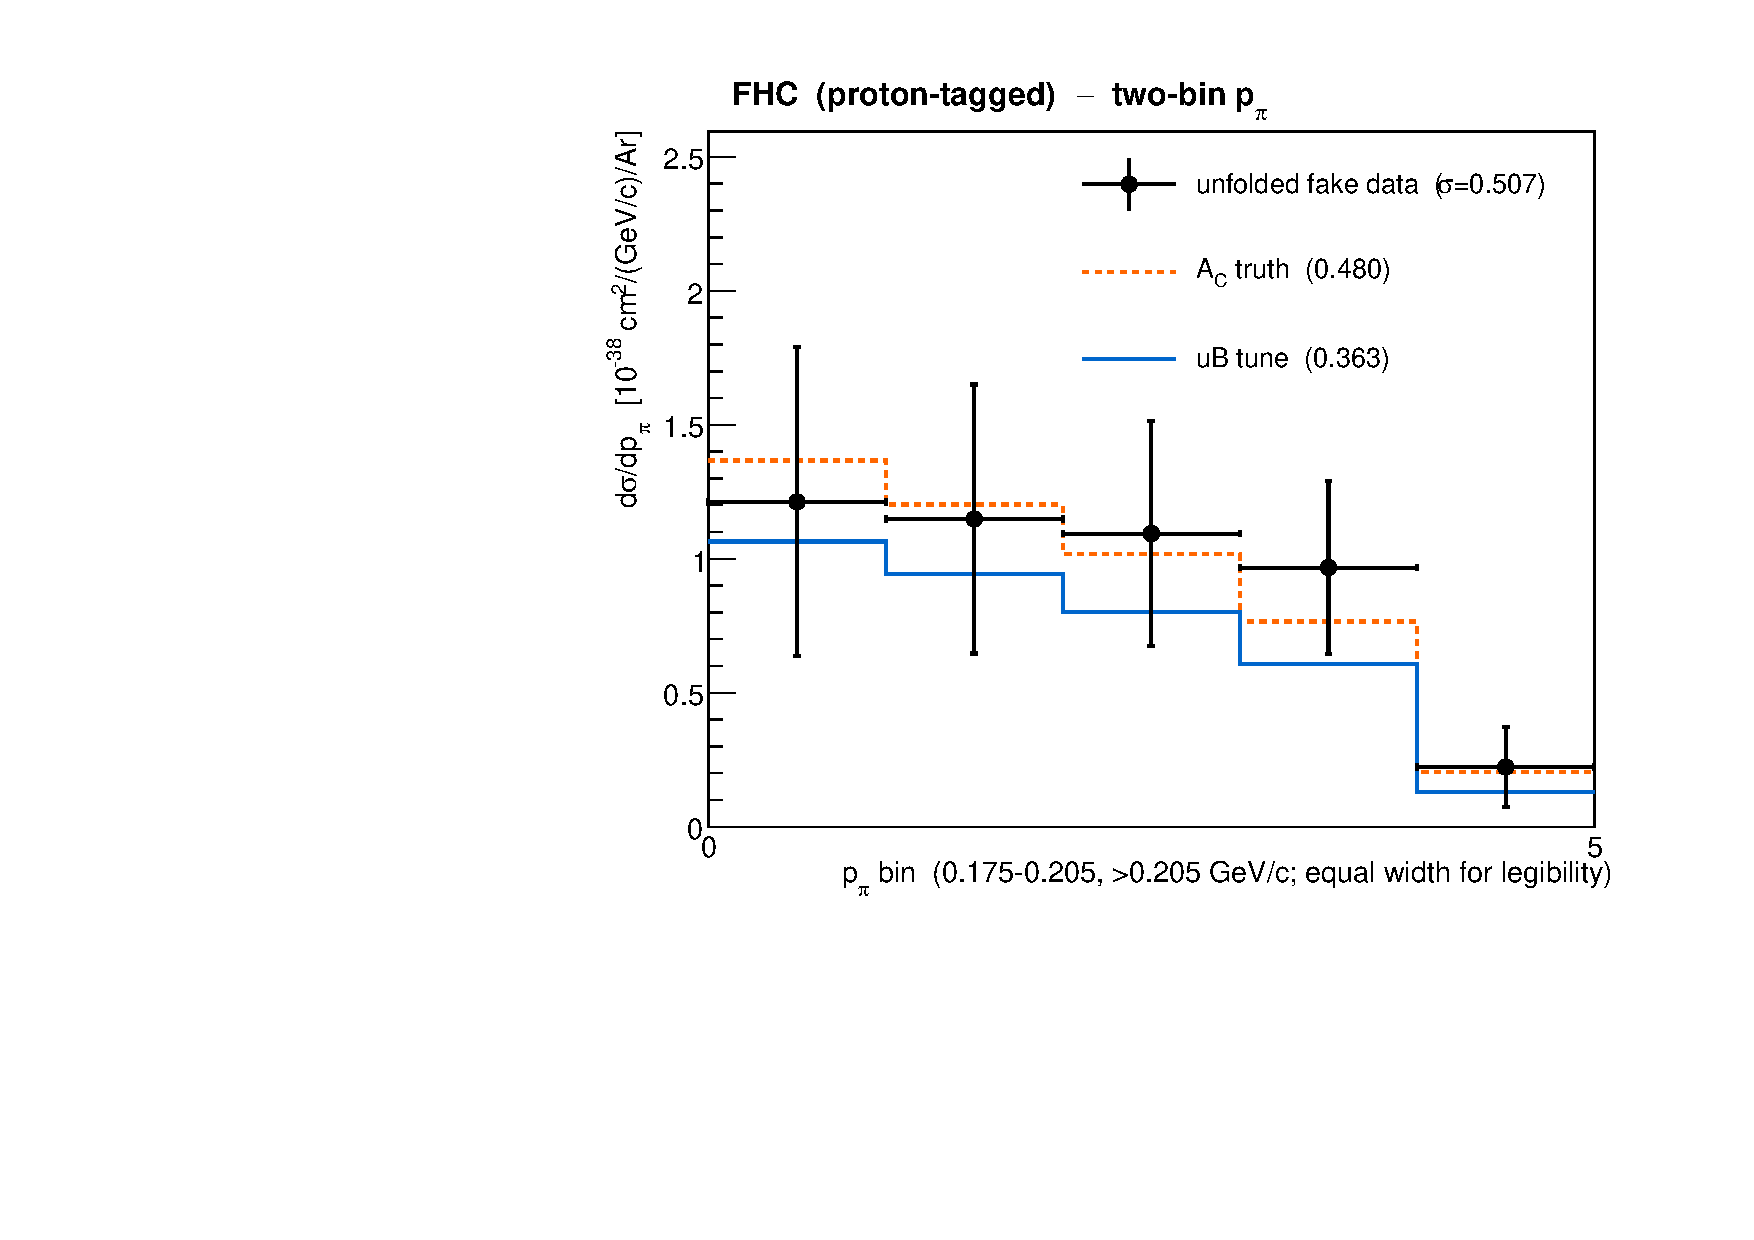
\includegraphics[width=\textwidth]{ppi2bin_xsec_1p_FHC}\caption{FHC}
  \end{subfigure}\hfill
  \begin{subfigure}[b]{0.32\textwidth}
    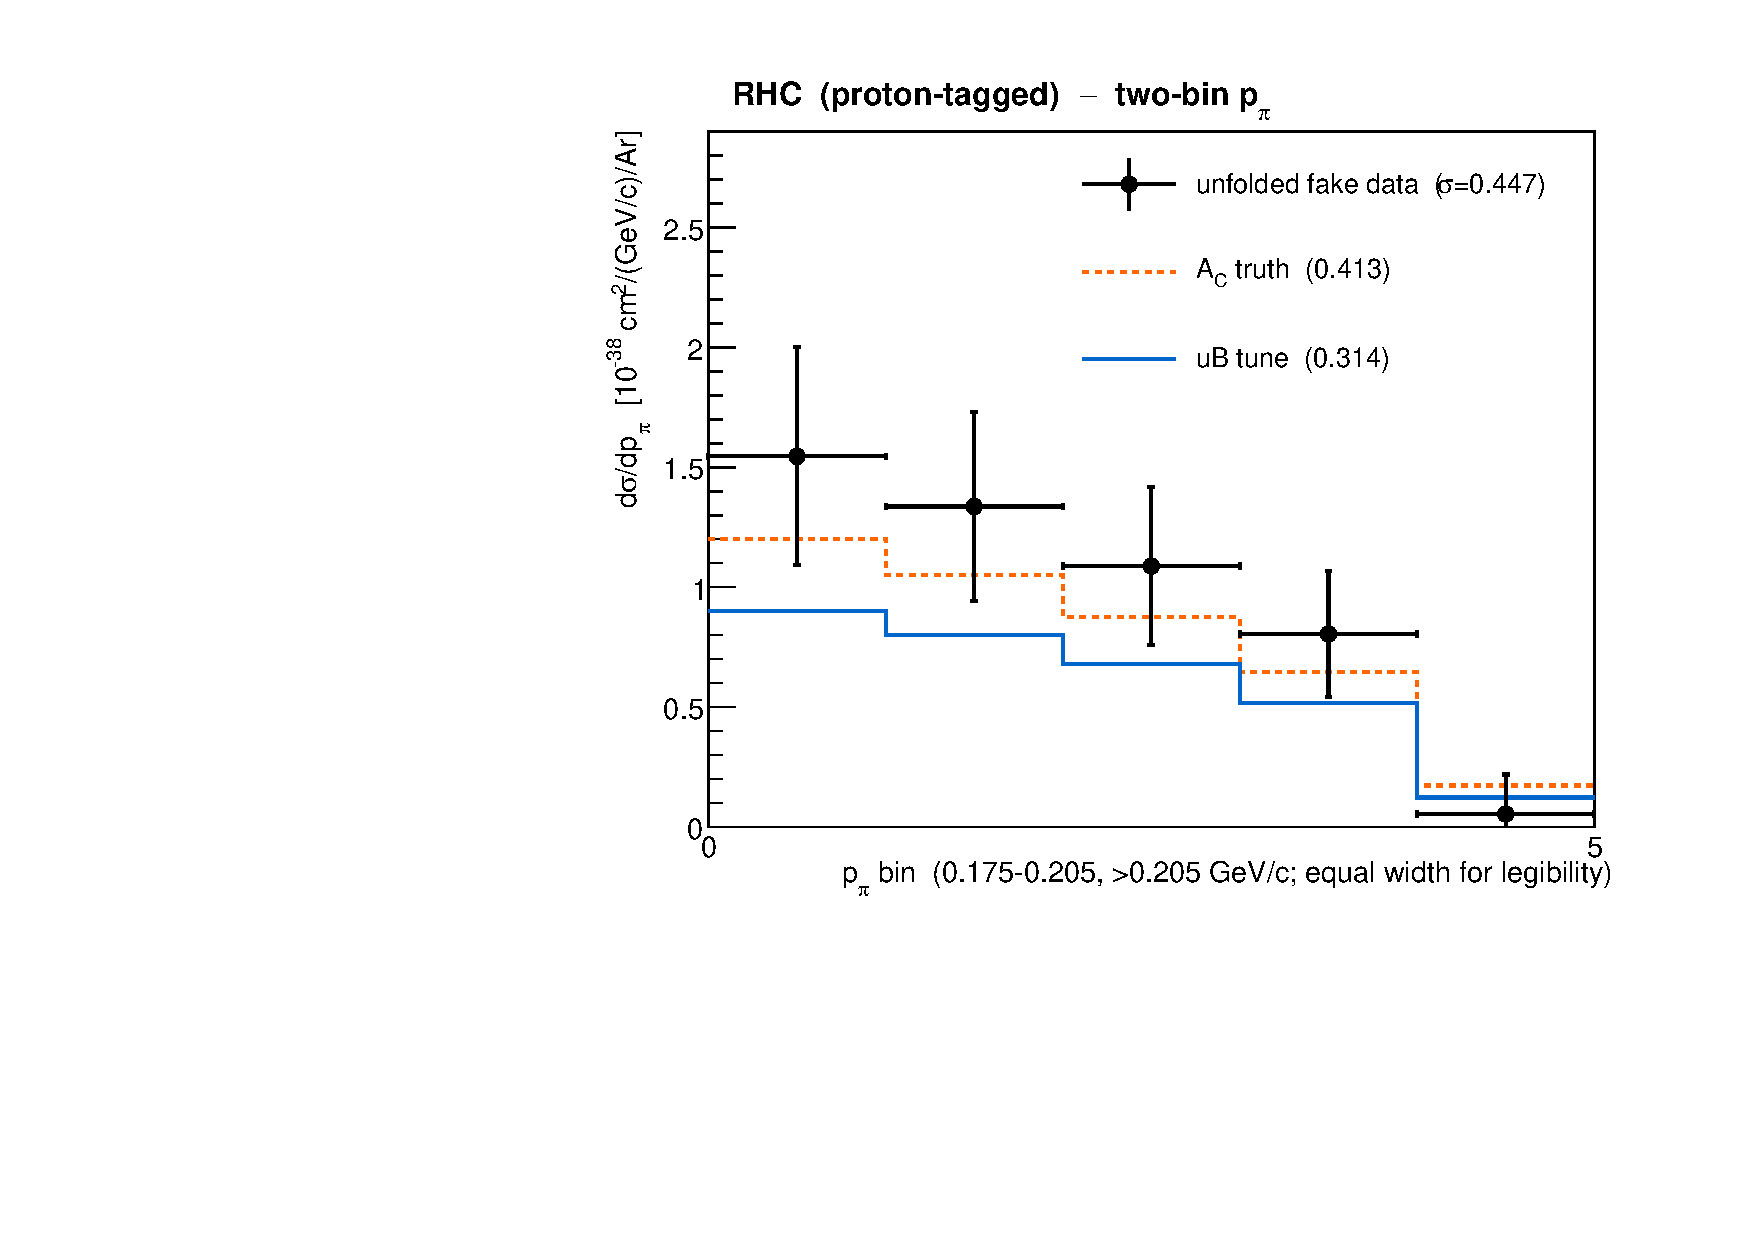
\includegraphics[width=\textwidth]{ppi2bin_xsec_1p_RHC}\caption{RHC}
  \end{subfigure}\hfill
  \begin{subfigure}[b]{0.32\textwidth}
    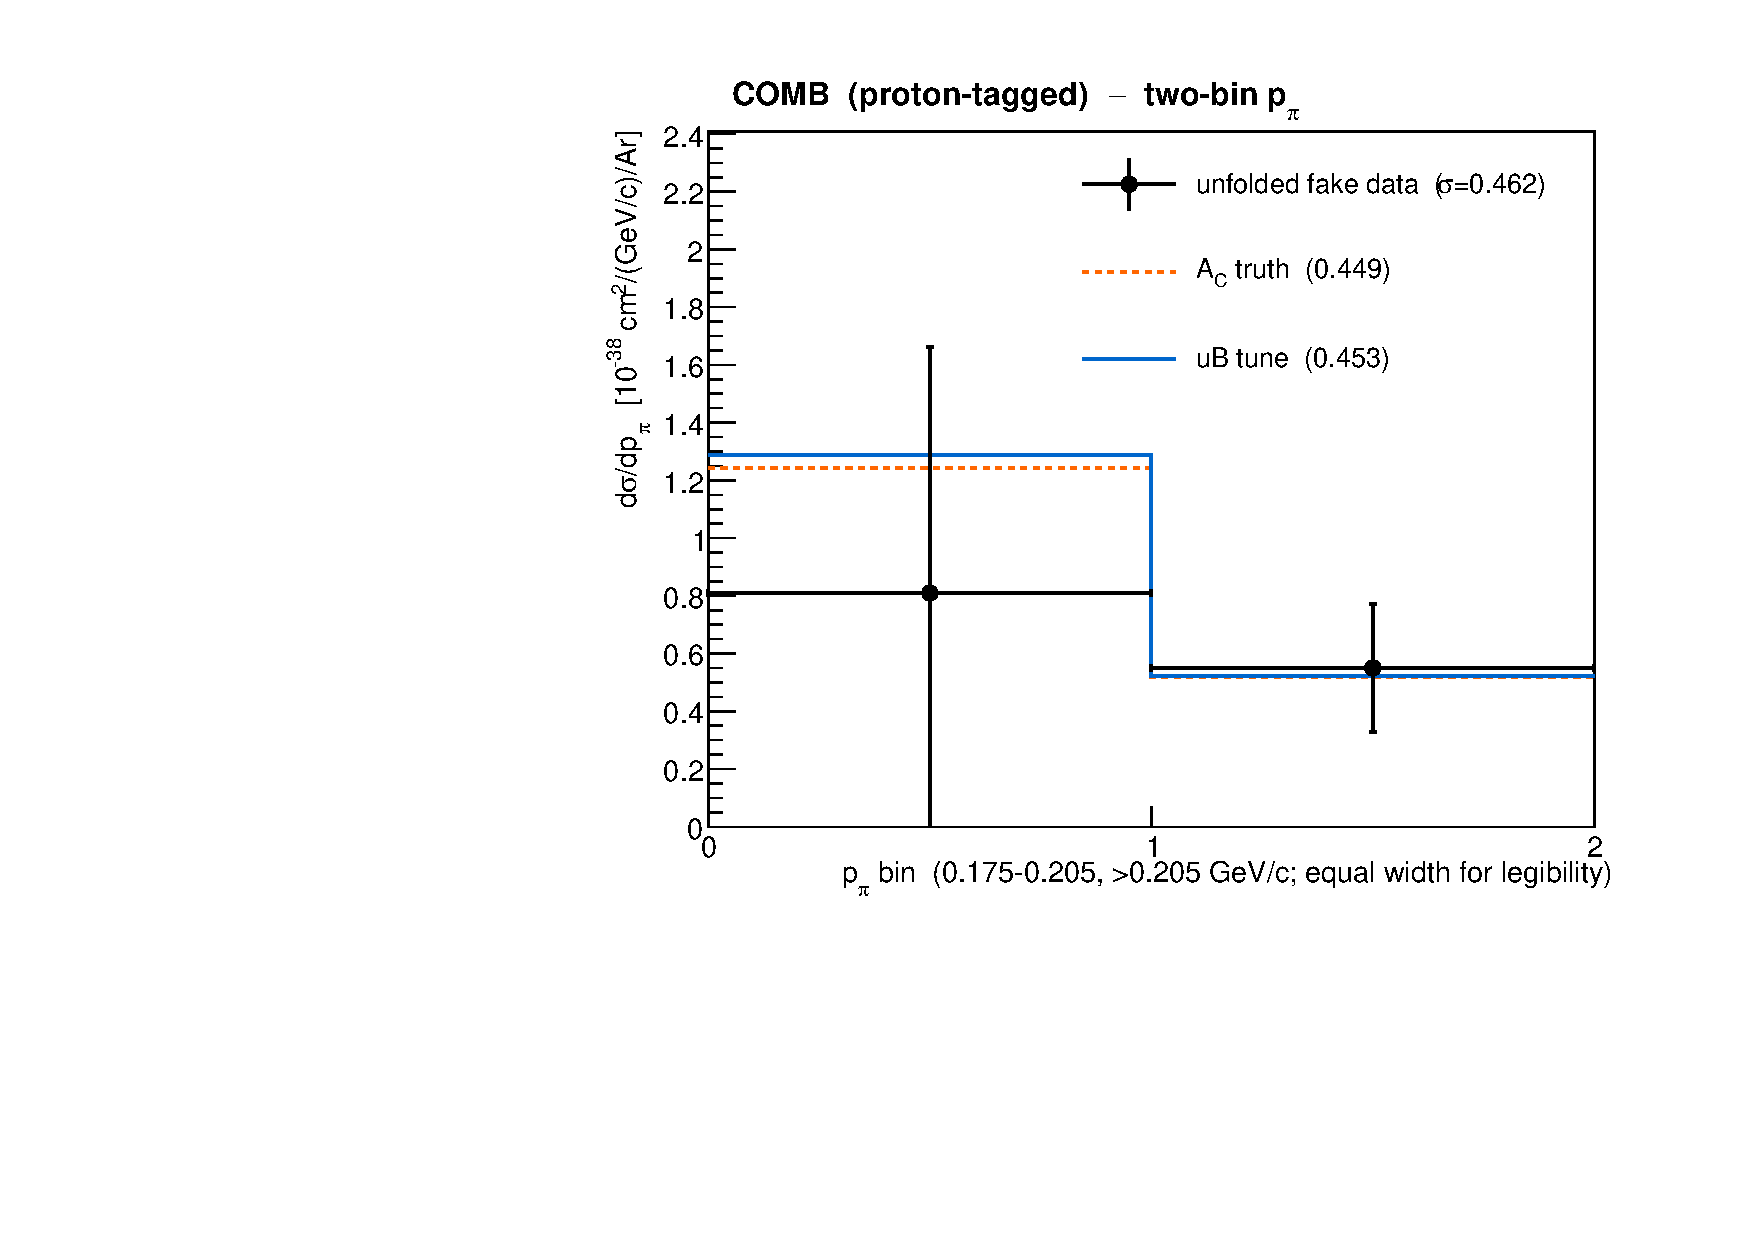
\includegraphics[width=\textwidth]{ppi2bin_xsec_1p_COMB}\caption{Combined}
  \end{subfigure}
  \caption{The two-bin $p_\pi$ cross section on the proton-tagged \texttt{CC1mu1pi1p}
    selection, the graphical form of Tab.~\ref{tab:ppi2bin_1p}. Same edges as the inclusive
    result of Fig.~\ref{fig:ppi2bin_xsec} so the two are directly comparable, and the bins
    are again drawn equal-width.}
  \label{fig:ppi2bin_1p}
\end{figure}

All three extractions close, with $\chi^2$ of $0.01$, $1.21$ and $0.40$ on two bins on the
current release. The $p_\pi$ differential cross section satisfies the field's
binning criterion in every bin of every beam configuration here, as it does on the inclusive
selection; the two are equivalent on that test, and the proton-tagged version is reported
because it belongs to the exclusive final state, not because it is required to make $p_\pi$
measurable.

\paragraph{The least-populated bin.} The RHC first bin unfolds to $0.37$ times its
$A_C$-smeared truth ($0.386\pm0.796$ against $1.056$) with an unremarkable closure
$\chi^2$ of $1.21/2$: a $0.8\sigma$ fluctuation on a bin whose uncertainty is twice its
content. Independent throws move it by more than $\pm1\sigma$. The bin holds too few
events to say anything, and any real-data value in it should be read with its uncertainty
and not its central value.

\noindent One caveat remains. The $0.205$~GeV/$c$ boundary was independently preferred
by the migration-level edge scan run on the proton-tagged selection
(\texttt{macros/ppi\_binning\_scan.C}, FHC; \texttt{logs/binning\_scan/1p\_fhc.txt}) as
well as by the inclusive scan, so it is not merely inherited. It was not, however,
re-optimised through a separate universe, covariance and unfolding production for every
candidate boundary, which would need its own universe construction per configuration
($\sim\!1$--$2$~h each); that is not expected to change the conclusion, since both bins
clear the criterion with margin in all three proton-tagged configurations.



\section{Rejected: extending the pion threshold below 0.175\,GeV/\textit{c}}
\label{sec:supp_lowppi}

\emph{The extension described here was tested and rejected; it is not part of the
measurement, whose threshold is $p_\pi>0.175$~GeV/$c$.}

\paragraph{The low-momentum bin, as a test.} The extension was implemented for $p_\pi$: a $[0.113,0.175]\GeVc$ bin is prepended to the pion-momentum binning,
lowering the measured phase space to the $\nu_e$ threshold. The truth-level signal
below $0.175\GeVc$ is recovered from the stored signal-component branches (the
reconstruction reproduces \texttt{MC\_Signal} above $0.175\GeVc$ to $0.4\%$, the
residual being the unstored kaon veto); $3323$ true signal events populate the new
bin. Its selection efficiency is $2.2\%$; an order of magnitude below the
$15$--$17\%$ of the standard bins (Table~\ref{tab:pithresh_eff}), as anticipated
from the reconstruction turn-on. Despite this, the Wiener--SVD extraction remains
well behaved with the bin included: the $M_A^\mathrm{RES}$ fake-data closure gives
$\chi^2/\mathrm{ndf}=1.41/6$ ($p=0.97$) and the flux term is unchanged
($17\%$ reco, $18.4\%$ unfolded, amplification $1.08\times$). The bin therefore
adds to the measurement, at the price of a large per-bin uncertainty driven by the
low efficiency.

The generator predictions have been regenerated on the six-bin scheme (the ppi
histogram uses $p_\pi>0.113$ while the other observables retain $p_\pi>0.175$,
mirroring the analysis). GENIE, NuWro and NEUT all provide the low bin; GiBUU could
not be re-binned as its generator-level event record was not retained, so it is
omitted from the extended $p_\pi$ comparison. Against the (fake) data the
generators give $\chi^2/\mathrm{ndf} = 11.1/6$ (GENIE, $p=0.09$), $7.0/6$ (NuWro,
$p=0.33$) and $6.3/6$ (NEUT, $p=0.39$): NEUT and NuWro describe the extended
spectrum well, while GENIE is mildly disfavoured, consistent with the known GENIE
over-prediction of low-momentum CC$\pi^{\pm}$ production.

\begin{center}\small
\captionof{table}{Selection efficiency per true $p_\pi$ bin with the low-momentum
  bin added. The new $[0.113,0.175]\GeVc$ bin sits at $2.2\%$, an order of
  magnitude below the standard bins.}
\label{tab:pithresh_eff}
\begin{tabular}{lccc}
\toprule
True $p_\pi$ [\GeVc] & $N_\mathrm{true}$ & $N_\mathrm{reco}$ & Efficiency \\
\midrule
$\mathbf{0.113}$--$\mathbf{0.175}$ (new) & 3323 & 74 & $\mathbf{2.2\%}$ \\
$0.175$--$0.250$ & 3368 & 526 & $15.6\%$ \\
$0.250$--$0.320$ & 2190 & 367 & $16.8\%$ \\
$0.320$--$0.420$ & 2831 & 479 & $16.9\%$ \\
$0.420$--$0.550$ & 2499 & 410 & $16.4\%$ \\
$0.550$--$1.000$ & 2933 & 429 & $14.6\%$ \\
\bottomrule
\end{tabular}
\end{center}

% =============================================================================

\section{Proton-tagged selection, binning and additional smearing}
\label{sec:supp_1pdetail}

The proton-tagged cut-flow, its per-observable binning study and its $A_C$ factors are
collected here rather than in the analysis note.  The note reports the extracted
proton-tagged cross sections and the reasons that sample is secondary scope; the material
below is the supporting detail.

\begin{figure}[H]
  \centering
  \begin{subfigure}[b]{0.32\textwidth}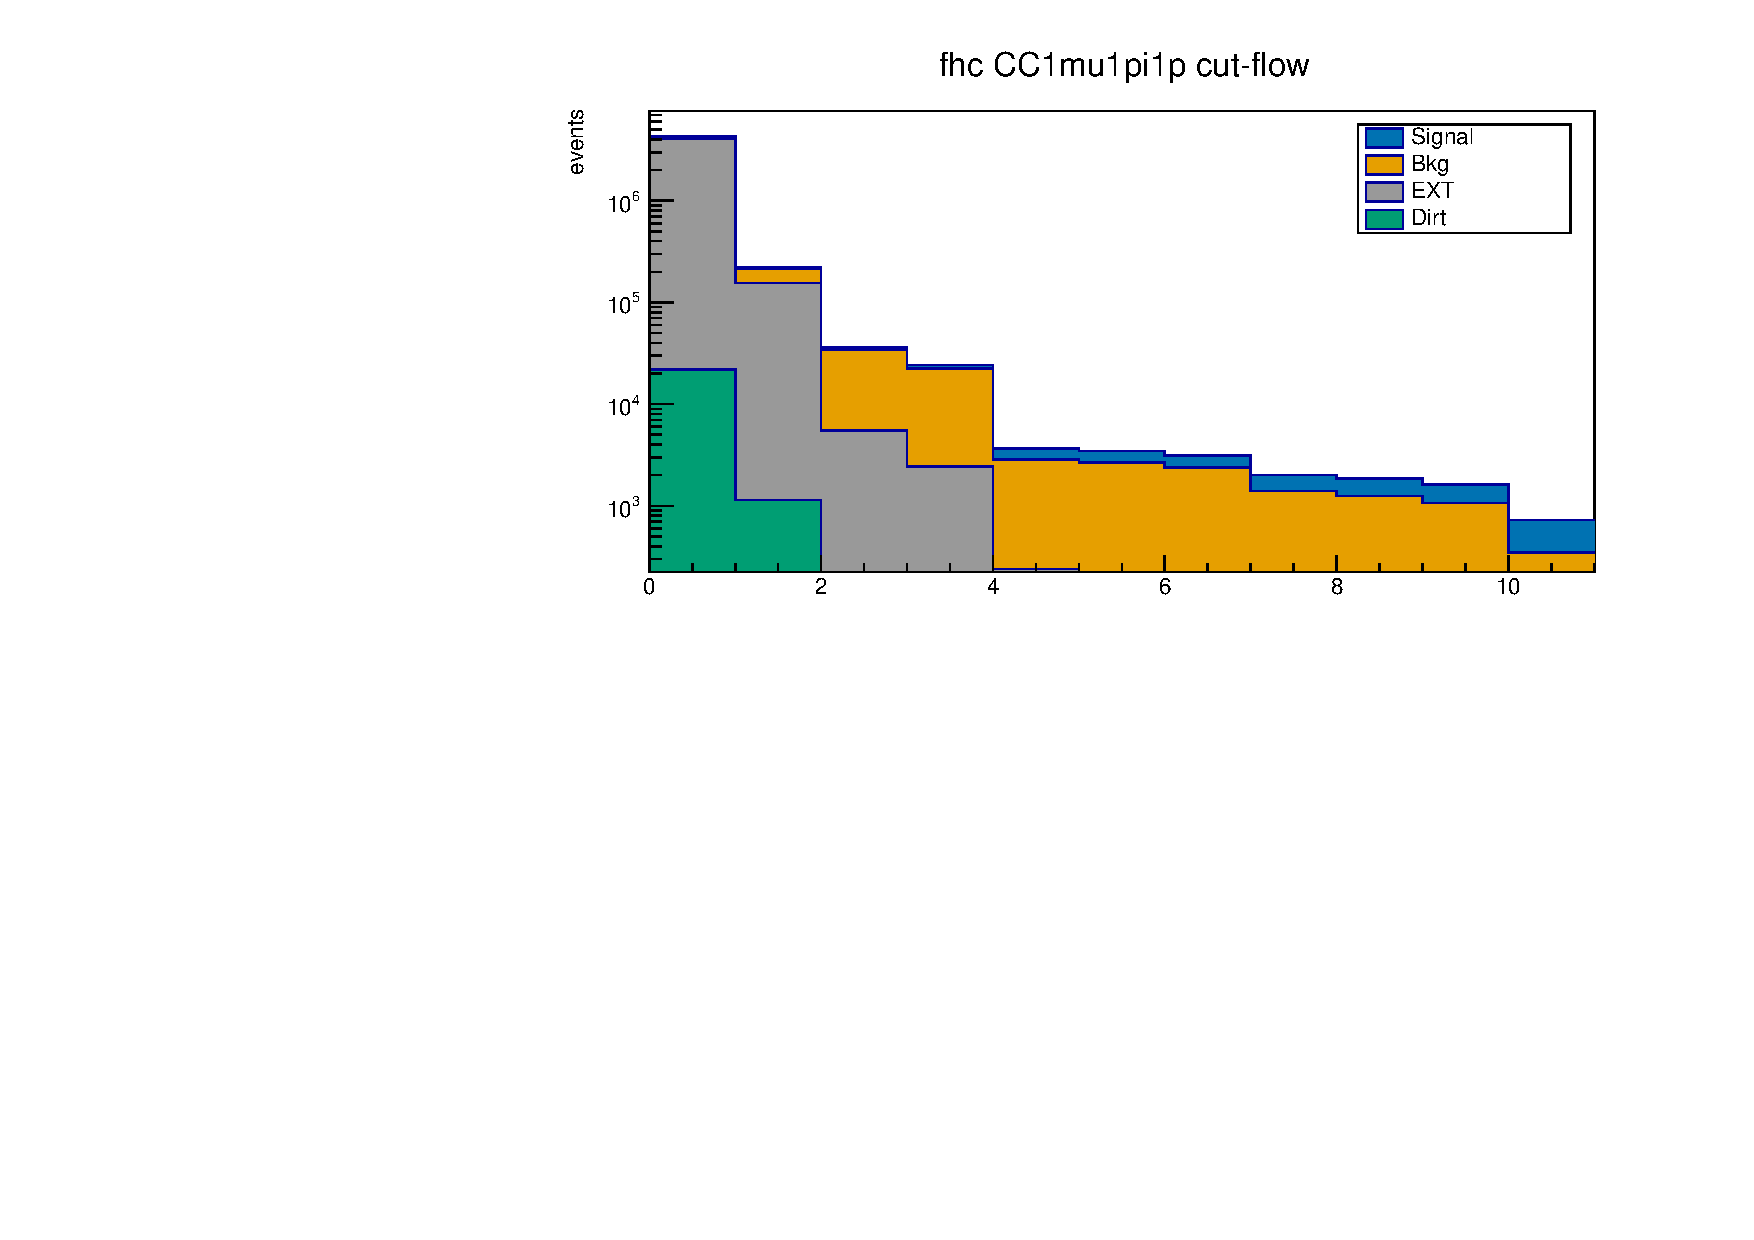
\includegraphics[width=\textwidth]{cutflow_yields_1p_fhc}\caption{FHC.}\end{subfigure}\hfill
  \begin{subfigure}[b]{0.32\textwidth}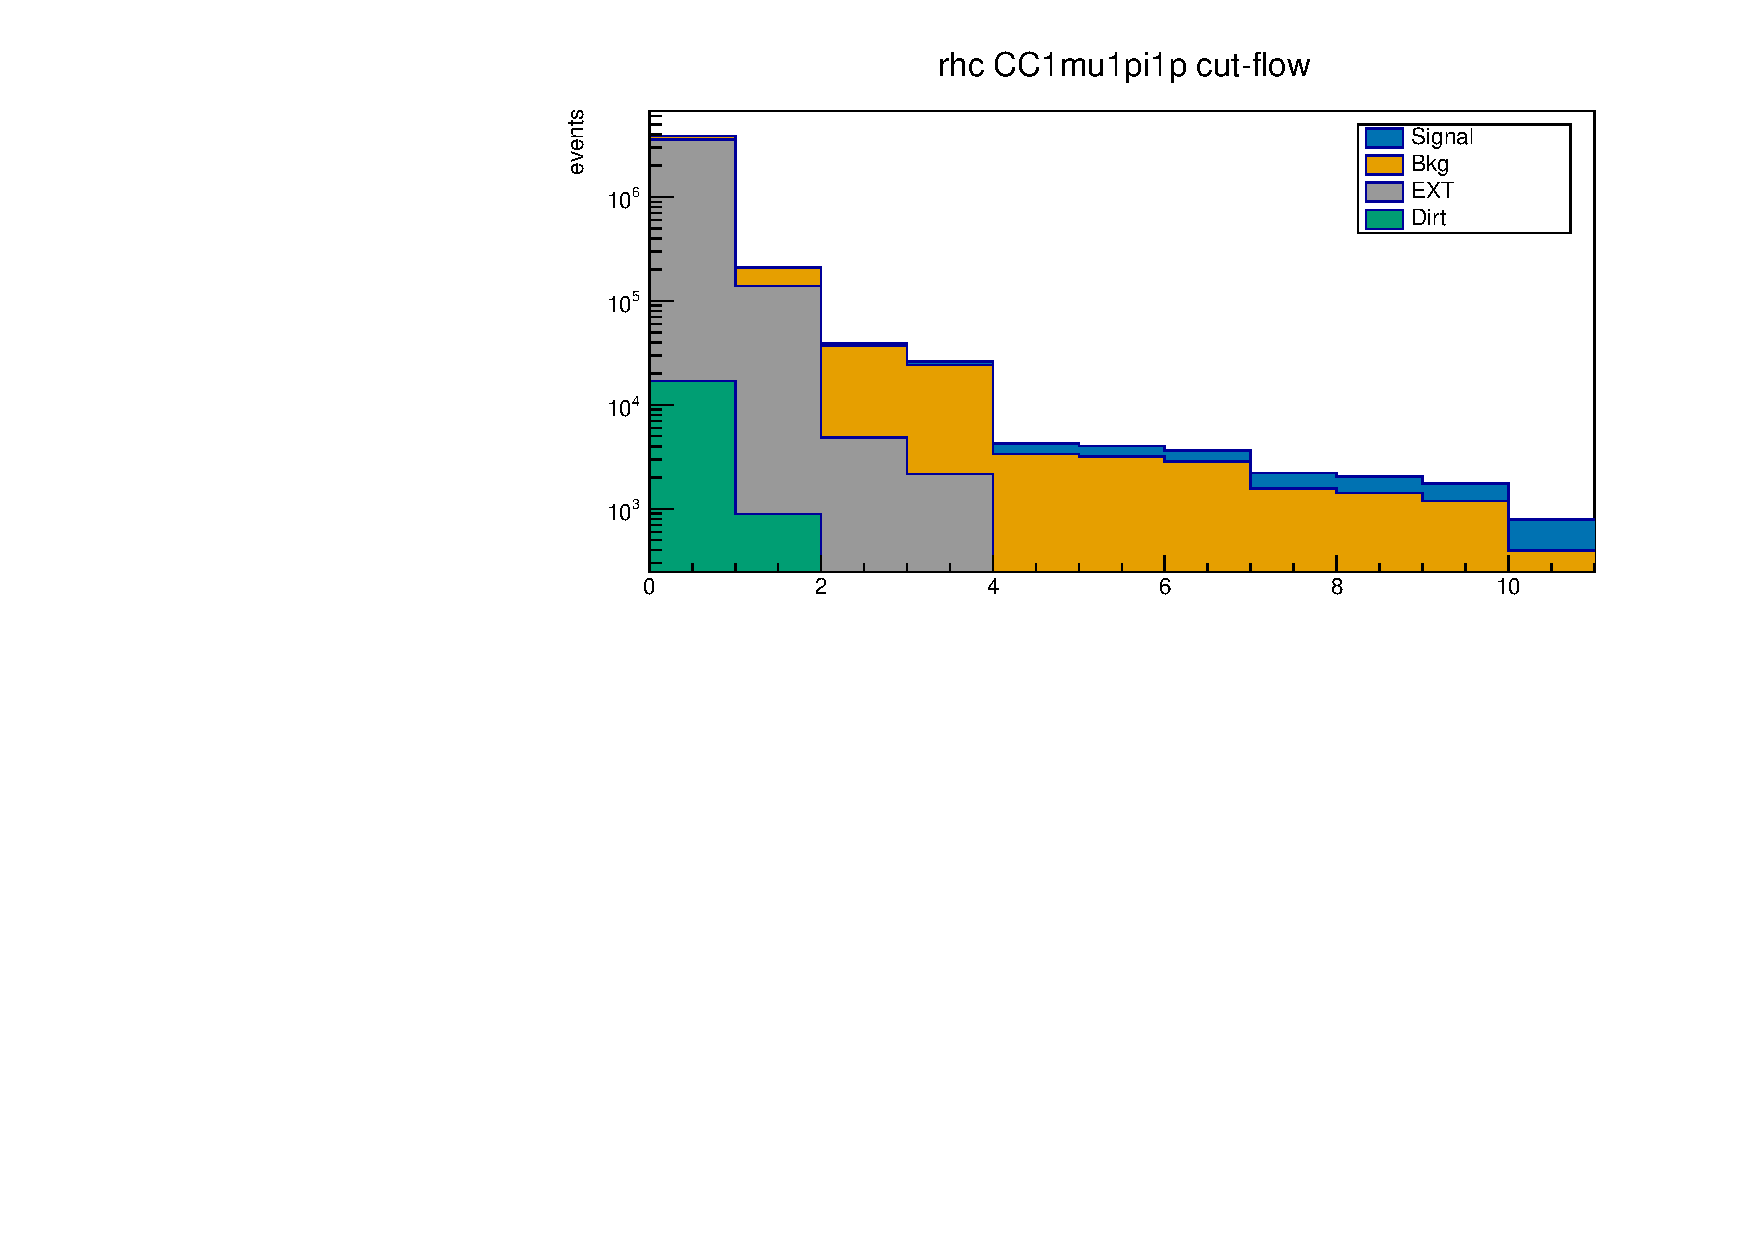
\includegraphics[width=\textwidth]{cutflow_yields_1p_rhc}\caption{RHC.}\end{subfigure}\hfill
  \begin{subfigure}[b]{0.32\textwidth}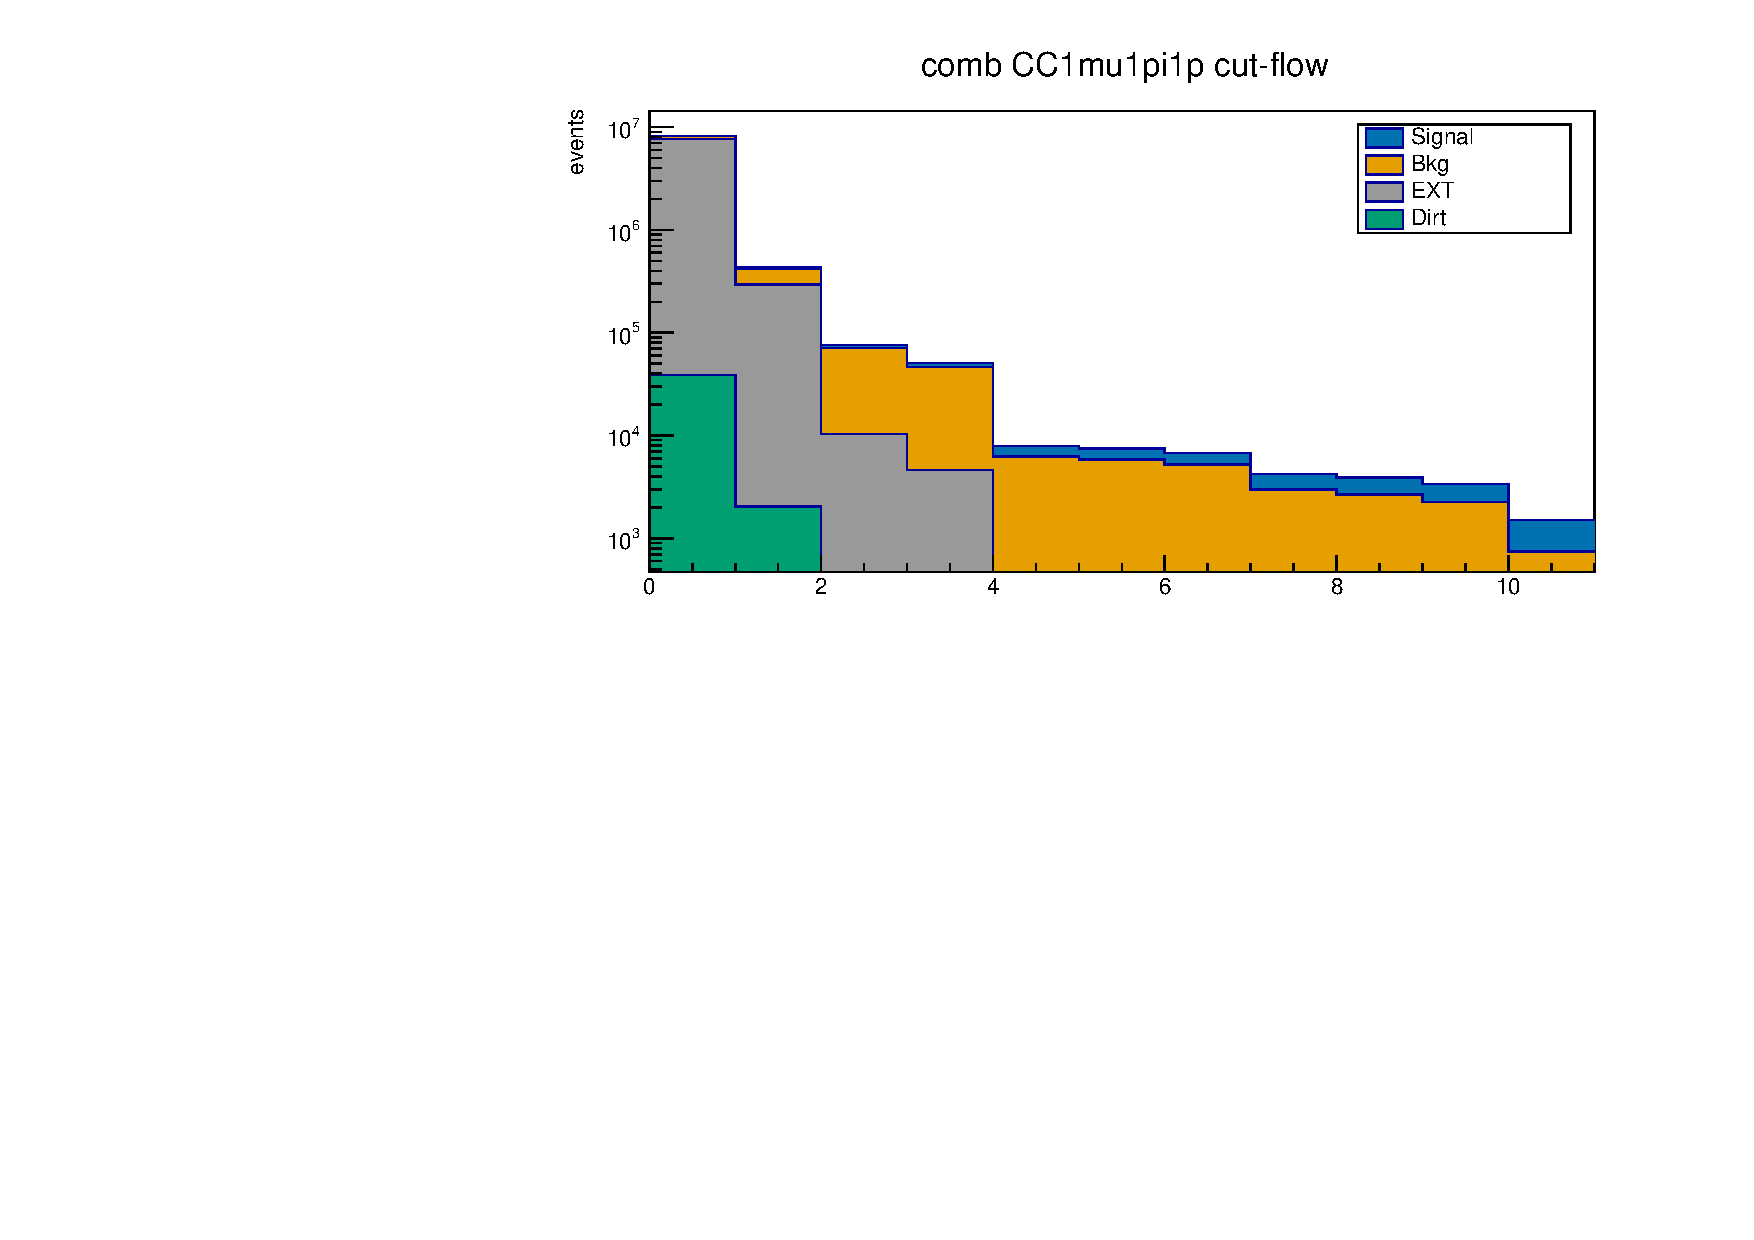
\includegraphics[width=\textwidth]{cutflow_yields_1p_comb}\caption{Combined.}\end{subfigure}
  \caption{Proton-tagged (\texttt{CC1mu1pi1p}) cut-flow yields at full exposure (log
    scale; MC-prediction stack, Okabe-Ito: signal blue, background orange, EXT grey,
    dirt green). The last stage, IdentProton, is the leading-proton identification that
    defines the subsample.}
  \label{fig:cutflow_1p}
\end{figure}

\begin{table}[H]
  \centering
  \caption{Proton-tagged (\texttt{CC1mu1pi1p}) cut-flow yields at full exposure for
    FHC, RHC and combined (MC prediction; data blind). Stages None--Nonprotons are the
    inherited inclusive selection with the proton-tagged signal definition; the final
    IdentProton stage adds the leading-proton identification. Signal/Bkg from the
    $\nu_\mu$ overlays POT-scaled per run, reprocessed with the proton-tagged selection
    and the full central-value weight under the safe-weight rule
    (\texttt{reprocess\_cutflow\_cf\_1p.sh}); EXT from the per-run beam-off
    samples scaled by the run gate ratios; dirt from the GENIE NuMI dirt overlay
    (\texttt{macros/cutflow\_yields\_1p.C}). The final row agrees with the
    proton-tagged cut-and-count check of the analysis note (\noteref{Table}{tab:cutcount}). Pred.\ $=$ Signal $+$ Bkg $+$ EXT $+$ Dirt. Eff.\ is the cumulative signal efficiency relative to the generated signal (the None stage, where all true signal is counted); Pur.\ $=$ Signal/Pred.}
  \label{tab:cutflow_1p}
  \small
  \begin{tabular}{lrrrrrrr}
    \toprule
    Cut & Signal & Bkg MC & EXT & Dirt & Pred. & Eff. [\%] & Pur. [\%] \\
    \midrule
    \multicolumn{8}{l}{\textit{FHC (Runs 1,2,4,5; $8.857\times10^{20}$~POT)}} \\
    None             & 3\,295 & 270\,438 & 4\,049\,292 & 21\,864 & 4\,344\,889 & 100.0 & 0.08 \\
    InFiducialVol    & 2\,763 & 61\,976 & 153\,533 & 1\,146 & 219\,418 & 83.9 & 1.3 \\
    Topological      & 2\,183 & 28\,864 & 5\,409 & 125 & 36\,580 & 66.2 & 6.0 \\
    MuonCandidate    & 1\,977 & 19\,865 & 2\,363 & 84 & 24\,288 & 60.0 & 8.1 \\
    ContainedPion    & 830 & 2\,608 & 223 & 16 & 3\,676 & 25.2 & 22.6 \\
    MuonIn3Planes    & 790 & 2\,472 & 185 & 11 & 3\,458 & 24.0 & 22.9 \\
    PionIn3Planes    & 733 & 2\,230 & 144 & 4.4 & 3\,112 & 22.3 & 23.6 \\
    ShowerCut        & 613 & 1\,294 & 108 & 3.8 & 2\,019 & 18.6 & 30.4 \\
    OpeningAngle     & 609 & 1\,207 & 41 & 1.2 & 1\,858 & 18.5 & 32.8 \\
    Nonprotons       & 550 & 1\,031 & 30 & 0.8 & 1\,612 & 16.7 & 34.1 \\
    \textbf{IdentProton} & \textbf{376} & \textbf{338} & \textbf{8.5} & \textbf{0.3} & \textbf{723} & \textbf{11.4} & \textbf{52.1} \\
    \multicolumn{8}{l}{\textit{RHC (Runs 1,2,3,4a,4b,4c; $1.108\times10^{21}$~POT)}} \\
    None             & 3\,427 & 288\,891 & 3\,560\,975 & 16\,958 & 3\,870\,250 & 100.0 & 0.09 \\
    InFiducialVol    & 2\,886 & 67\,416 & 139\,122 & 889 & 210\,312 & 84.2 & 1.4 \\
    Topological      & 2\,318 & 31\,870 & 4\,767 & 97 & 39\,052 & 67.7 & 5.9 \\
    MuonCandidate    & 2\,111 & 21\,962 & 2\,090 & 65 & 26\,227 & 61.6 & 8.0 \\
    ContainedPion    & 882 & 3\,181 & 191 & 12 & 4\,267 & 25.7 & 20.7 \\
    MuonIn3Planes    & 842 & 3\,015 & 158 & 8.3 & 4\,023 & 24.6 & 20.9 \\
    PionIn3Planes    & 784 & 2\,739 & 121 & 3.4 & 3\,648 & 22.9 & 21.5 \\
    ShowerCut        & 647 & 1\,480 & 86 & 2.9 & 2\,216 & 18.9 & 29.2 \\
    OpeningAngle     & 643 & 1\,384 & 33 & 0.9 & 2\,060 & 18.8 & 31.2 \\
    Nonprotons       & 573 & 1\,162 & 23 & 0.6 & 1\,759 & 16.7 & 32.6 \\
    \textbf{IdentProton} & \textbf{391} & \textbf{388} & \textbf{7.1} & \textbf{0.2} & \textbf{786} & \textbf{11.4} & \textbf{49.8} \\
    \multicolumn{8}{l}{\textit{Combined FHC$+$RHC ($1.994\times10^{21}$~POT)}} \\
    None             & 6\,721 & 559\,329 & 7\,610\,266 & 38\,822 & 8\,215\,139 & 100.0 & 0.08 \\
    InFiducialVol    & 5\,649 & 129\,392 & 292\,655 & 2\,035 & 429\,731 & 84.0 & 1.3 \\
    Topological      & 4\,501 & 60\,734 & 10\,176 & 221 & 75\,632 & 67.0 & 6.0 \\
    MuonCandidate    & 4\,088 & 41\,826 & 4\,453 & 148 & 50\,515 & 60.8 & 8.1 \\
    ContainedPion    & 1\,712 & 5\,790 & 414 & 28 & 7\,943 & 25.5 & 21.6 \\
    MuonIn3Planes    & 1\,632 & 5\,487 & 343 & 19 & 7\,481 & 24.3 & 21.8 \\
    PionIn3Planes    & 1\,518 & 4\,969 & 266 & 7.8 & 6\,760 & 22.6 & 22.5 \\
    ShowerCut        & 1\,260 & 2\,774 & 194 & 6.7 & 4\,235 & 18.7 & 29.7 \\
    OpeningAngle     & 1\,251 & 2\,591 & 74 & 2.2 & 3\,918 & 18.6 & 31.9 \\
    Nonprotons       & 1\,123 & 2\,193 & 53 & 1.5 & 3\,371 & 16.7 & 33.3 \\
    \textbf{IdentProton} & \textbf{768} & \textbf{726} & \textbf{16} & \textbf{0.5} & \textbf{1\,509} & \textbf{11.4} & \textbf{50.9} \\
    \bottomrule
  \end{tabular}
\end{table}

\begin{table}[H]
  \centering
  \caption{Released binning of the eight W/TKI and angular proton-tagged observables, read from the
    data release (\texttt{curves\_1p\_*.tsv}). The two mass variables keep six
    equal-population bins chosen from the validated true-signal distributions, with the
    last bin open at truth level (the upper edge listed is the plotting boundary); the four
    TKI variables use the coarsened two-bin scheme adopted after the six-bin scheme was
    found to sit inside the resolution (\S\ref{sec:w_binning}). $W_{\pi p}$ brackets the
    $\Delta(1232)$ peak but its differential shape is withdrawn. The five inherited kinematic
    observables ($p_\mu$, $p_\pi$, $\cos\theta_\mu$, $\cos\theta_\pi$, $\theta_{\mu\pi}$)
    use the inclusive-analysis binning of \noteref{Appendix}{app:binning} unchanged.}
  \label{tab:wtki_binning}
  \footnotesize
  \begin{tabular}{llcl}
    \toprule
    Observable & Definition & Bins & Released bin edges \\
    \midrule
    $W_{\pi p}$        & $M(\pi p)$, direct        & 6 (withdrawn) & $1.08,\,1.19,\,1.23,\,1.27,\,1.34,\,1.47,\,2.9$~GeV/$c^2$ \\
    $W_\mathrm{had}$   & calorimetric              & 6 & $0,\,0.78,\,1.08,\,1.21,\,1.31,\,1.44,\,2.74$~GeV/$c^2$ \\
    $\delta p_T$       & $|\vec p_T^{\,\mu}+\vec p_T^{\,\mathrm{had}}|$ & 2 & $0,\,0.3,\,2.5$~GeV/$c$ \\
    $\delta\alpha_T$   & TKI angle                 & 2 & $0,\,120,\,180^\circ$ \\
    $\delta\phi_T$     & TKI angle                 & 2 & $0,\,50,\,180^\circ$ \\
    $p_n$              & inferred nucleon momentum & 2 & $0,\,0.375,\,2$~GeV/$c$ \\
    $\theta_p$         & proton polar angle        & 4$^{\dagger}$ & $0,\,0.659,\,1.068,\,1.539,\,\pi$~rad \\
    $\theta_{\pi p}$   & $\pi$--$p$ opening angle  & 3$^{\dagger}$ & $0,\,1.193,\,2.010,\,\pi$~rad \\
    \bottomrule
  \end{tabular}
  \par\smallskip\noindent{\footnotesize $^{\dagger}$ Proposed secondary scope, added 2026-09-18;
    not part of the 2026-09-06 release. $\theta_p$'s edges are derived on the RHC chain.}
\end{table}



\subsection{Additional smearing in the proton-tagged observables}
\label{sec:acwtki}

Because the Wiener--SVD additional-smearing matrix $A_C$ is not norm-preserving, each
observable's predictions are rescaled by a different factor when they are brought into the
measurement space. Table~\ref{tab:acwtki} gives that factor, measured as the ratio of the
$A_C$-smeared to the truth-level generator integral, for the six proton-tagged observables.
Its dominant behaviour is set by the response and the binning; the exact factor is
prediction-dependent, and for the tested generators GENIE and GiBUU agree to a few per
cent throughout.

On the current release the six proton-tagged observables are suppressed by similar
amounts, $0.61$--$0.79$ (Table~\ref{tab:acwtki}): the two-bin TKI variables and
$W_{\pi p}$ sit at $0.70$--$0.79$ and the six-bin $W_\mathrm{had}$, the most affected, at
$0.61$. Sharpness alone does not drive the suppression: $W_{\pi p}$ is the sharpest
distribution measured here (the ratio of its largest to smallest bin is $\sim\!36$) yet is
suppressed no more than the TKI variables, because $A_C$ removes structure that the
\emph{response} cannot resolve and $W_{\pi p}$ is built from directly measured pion and
proton momenta with equal-population bins that track the $\Delta(1232)$ peak. No
observable is enhanced by $A_C$ (a physical smearing cannot amplify; an amplification
would signal a mis-specified regularisation, \S\ref{sec:thetavar}). The suppression is applied identically to data, tune and generators, so model
comparisons read off any panel are made on equal footing.

\begin{table}[H]
  \centering
  \caption{Mean $A_C$ row sum for the proton-tagged observables (FHC), from the released
    matrices \texttt{A\_C\_1p\_FHC5\_*.tsv}, release 2026-09-06; equal to the ratio of the
    $A_C$-smeared to the truth-level integral for a flat prediction. The inclusive
    observables are given for scale.}
  \label{tab:acwtki}
  \par\smallskip\noindent{\footnotesize $^{\dagger}$ From the 2026-09-18 extraction rather than the
    2026-09-06 data release, which does not contain these observables.}
  \begin{tabular}{lc}
      \toprule
      Observable & mean $A_C$ row sum \\
      \midrule
      $p_n$              & $0.79$ \\
      $\theta_p$$^{\dagger}$         & $0.73$ \\
      $\theta_{\pi p}$$^{\dagger}$      & $0.61$ \\
      $\delta\alpha_T$   & $0.79$ \\
      $W_{\pi p}$        & $0.75$ \\
      $\delta\phi_T$     & $0.72$ \\
      $\delta p_T$       & $0.70$ \\
      $W_\mathrm{had}$   & $0.61$ \\
      \midrule
      \multicolumn{2}{p{0.72\textwidth}}{\emph{Computed from the released matrices
        (\texttt{A\_C\_1p\_FHC5\_*.tsv}). The values span $0.61$--$0.79$, a range of
        $0.18$, so differences in smearing cannot order the generator $\chi^2$ across
        observables.}} \\
      \bottomrule
    \end{tabular}
\end{table}



% =============================================================================


\section{Hadronic mass, model comparison, and estimator surveys}
\label{sec:supp_w}

\subsection{The $W$ binnings are finer than the resolution}
\label{sec:w_binning}

$W_{\pi p}$ shows the least model tension of the proton-tagged observables. The cause is
not physics.

The bin edges were chosen for equal population, six bins of roughly equal content, without
reference to the resolution. Measured on selected signal, FHC Runs 1/2/4:

\begin{center}\small
\begin{tabular}{lcc}
\toprule
 & $W_{\pi p}$ & $W_\mathrm{had}$ \\\midrule
residual RMS [GeV/$c^2$]           & $0.142$ & $0.283$ \\
robust half-width ($16$--$84\%$)   & $0.101$ & $0.177$ \\
bias (mean reco $-$ true)          & $\mathbf{-0.111}$ & $-0.032$ \\\midrule
narrowest analysis bin             & $\mathbf{0.040}$ & $0.100$ \\
widest analysis bin                & $1.430$ & $1.300$ \\
width ratio                        & $\mathbf{35.7}$ & $13.0$ \\
\bottomrule
\end{tabular}
\end{center}

\noindent The second and third $W_{\pi p}$ bins are $40$~MeV/$c^2$ wide against a resolution
of $101$--$142$~MeV/$c^2$: they are two to three times narrower than the detector can
resolve. The bias alone, $-111$~MeV/$c^2$, is larger than three of the six bin widths. The
migration diagonals follow directly, $87.6/22.3/11.7/12.0/10.0/2.3\%$: only the first bin
is measured, and the top bin at $2.3\%$ is essentially unmeasured.

This is the same failure as the five-bin $p_\pi$ scheme, and for the same underlying reason.
$W_{\pi p}$ is reconstructed from the pion and proton momenta, so it inherits the saturation
of the range-based pion momentum described in \S\ref{sec:ppi_bias}; its resolution cannot be
better than that of its inputs.

An exhaustive edge scan, the same procedure and criterion used for $p_\pi$, gives:

\begin{center}\small
\begin{tabular}{llc}
\toprule
scheme & diagonals & verdict \\\midrule
current, six bins            & $87.6 / 22.3 / 11.7 / 12.0 / 10.0 / 2.3\%$ & 1 of 6 usable \\
best two bins (split $1.15$) & $\mathbf{83.2 / 77.9\%}$ & \textbf{both usable} \\
best three bins              & $83.2 / 49.7 / 45.9\%$ & fails \\
best four bins               & $83.2 / 45.0 / 28.2 / 28.2\%$ & fails \\
\bottomrule
\end{tabular}
\end{center}

\noindent As with $p_\pi$, two bins is not merely the best option but the only one that
satisfies the criterion, and the first bin is thin ($137$ selected signal events, against a
floor of $100$). The implication for the model comparison is direct: a low generator $\chi^2$ at six
bins would reflect a binning that cannot resolve the differences between generators, not
agreement between them. The same test should be applied to $W_\mathrm{had}$, whose upper bins are also narrower
than its $177$~MeV/$c^2$ half-width, before either $W$ result is quoted as a shape
measurement. \emph{[Open: the $W_\mathrm{had}$ edge scan has not been run; $W_\mathrm{had}$
is released at six bins with its closure and generator overlays, and its shape should be
read with this caveat (analysis note, Limitations).]}

\paragraph{Adopted scheme: two bins split at $1.15$~GeV/$c^2$.} The boundary is more tightly
constrained than it was for $p_\pi$, where anything between roughly $0.19$ and $0.22$ worked.
Here only one choice satisfies both the diagonal criterion and the $100$-event floor:

\begin{center}\small
\begin{tabular}{lccr l}
\toprule
boundary [GeV/$c^2$] & bin 1 & bin 2 & $N$(bin 1) & \\\midrule
$1.13$          & $76.5\%$ & $88.0\%$ & $51$   & below the event floor \\
$\mathbf{1.15}$ & $\mathbf{83.2\%}$ & $\mathbf{77.9\%}$ & $\mathbf{137}$ & \textbf{adopted} \\
$1.17$          & $86.8\%$ & $66.8\%$ & $266$  & bin 2 just fails \\
$1.19$          & $87.6\%$ & $56.0\%$ & $468$  & fails \\
$1.23$          & $91.7\%$ & $37.6\%$ & $1114$ & fails \\
\bottomrule
\end{tabular}
\end{center}

\noindent Moving the boundary up buys population in the first bin at the direct expense of
the second: the two diagonals trade against each other steeply, and the window in which both
exceed $0.68$ is only about $\pm0.01$~GeV/$c^2$ wide. That narrowness is itself a
consequence of the resolution being comparable to the full width of the peak region.

Two consequences should be carried with the result. First, \textbf{the first bin is thin},
$137$ selected signal events against a floor of $100$, so its statistical uncertainty will be
large once systematics are folded in; the $p_\pi$ first bin, with $469$ events, carries $77\%$ (Table~\ref{tab:ppi2bin_1p}). Second, if that proves too sparse in practice, $1.17$ is the natural
fallback: it doubles the population for a bin-2 diagonal of $66.8\%$, marginally below
threshold, which is a defensible trade to state explicitly rather than a criterion to fail
silently.

The scheme is implemented in \texttt{configs/ccpi1p\_Wpipr\_bin\_config\_2bin.txt}, with the
reasoning recorded alongside it in a companion \texttt{.README}. Running it through the
extraction settled the question (\S\ref{sec:wpipr_limits}): the two-bin scheme meets the migration
criterion but leaves only about $137$ selected signal events in the first bin, which the
Wiener filter then suppresses, driving $A_C$ towards rank one for statistical rather than
algebraic reasons.  Widening the first bin restores its population at the cost of the
upper-bin diagonal, and no scanned edge satisfies both requirements at once.

The apparent $W_{\pi p}$ agreement therefore does \emph{not} survive a binning the detector
can resolve, and the differential shape is withdrawn: at this exposure the proton-tagged
sample supports an integrated cross section.  $W_\mathrm{had}$ carries the same limitation,
since it depends on the same pion momentum.




\subsection{What limits $W_{\pi p}$, and what can be done about it}
\label{sec:wpipr_limits}

The two-bin $W_{\pi p}$ scheme of \S\ref{sec:w_binning} was built and run. It does not work,
for a reason distinct from the six-bin failure, and the investigation that followed settles
what the pion momentum can and cannot deliver.

\paragraph{The two-bin extraction fails on statistics.} The \emph{response} behaves exactly
as designed: the framework returns migration diagonals of $0.802$ and $0.773$, matching the
truth-level scan, and the closure is acceptable at $\chi^2=1.17/2$ ($p=0.56$). The
\emph{extraction} nonetheless carries almost no shape information, because $A_C$ collapses:

\noindent\emph{(Matrices from the pass in which the two-bin $W_{\pi p}$ scheme was run,
written with true bins as rows; the two $p_\pi$ rows are the same-pass comparison, and the
released inclusive $p_\pi$ matrix is that of Fig.~\ref{fig:ppi2bin_AC}.)}
\begin{center}\small
\begin{tabular}{lcc}
\toprule
two-bin scheme & $A_C$ & $s_2/s_1$ \\\midrule
$W_{\pi p}$, first bin $N=137$      & $\bigl(\begin{smallmatrix} 0.018 & -0.410 \\ 0.034 & 0.892\end{smallmatrix}\bigr)$ & $\mathbf{0.031}$ \\
$p_\pi$ proton-tagged, $N=469$      & $\bigl(\begin{smallmatrix} 0.498 & -0.089 \\ 0.013 & 0.854\end{smallmatrix}\bigr)$ & $0.577$ \\
$p_\pi$ inclusive, $N=1056$         & $\bigl(\begin{smallmatrix} 0.594 & -0.382 \\ 0.011 & 0.891\end{smallmatrix}\bigr)$ & $0.528$ \\
\bottomrule
\end{tabular}
\end{center}

\noindent The top-left entry is $0.018$: $A_C$ passes under two per cent of the first bin and
takes $-0.41$ from the second. This is a rank-one collapse of the kind described in
\S\ref{sec:thetavar}, but its cause is statistical rather than a defective regulariser. With
$137$ events the first bin has such poor signal-to-noise that the Wiener filter suppresses
that mode almost entirely, and the ordering across the three schemes, $137\to0.031$,
$469\to0.577$, $1056\to0.528$, follows population rather than anything geometric.

$W_{\pi p}$ is therefore caught between two requirements. Bins narrow enough to satisfy the
response criterion leave the first bin too sparse to unfold; bins wide enough for a stable
unfold ($1.19$ gives $468$ events, matching the $p_\pi$ case that works) fail the criterion at
$56\%$.

\paragraph{No binning escapes it.} The conclusion does not rest on the one scheme that was
tried. Scanning \emph{every} two- and three-bin scheme with edges between $1.12$ and
$1.70$~GeV/$c^2$ (FHC Run1$+$2$+$4, $3505$ selected signal events) finds none that keeps both
a migration diagonal above $0.68$ and adequate statistics in every bin:

\begin{center}\small
\begin{tabular}{lccc}
\toprule
two-bin edge & $N_1 / N_2$ & diag$_1$ / diag$_2$ & \\\midrule
$1.15$ & $137 / 3367$  & $0.832 / 0.779$ & first bin too sparse \\
$1.18$ & $351 / 3153$  & $0.866 / 0.611$ & \\
$1.24$ & $1298 / 2206$ & $0.930 / 0.347$ & \\
$1.27$ (median) & $1744 / 1760$ & $0.951 / \mathbf{0.261}$ & upper bin unusable \\
$1.45$ & $2966 / 538$  & $0.993 / 0.030$ & \\
\bottomrule
\end{tabular}
\end{center}

\noindent The trend exposes the mechanism. Reconstructed $W_{\pi p}$ is biased about
$111$~MeV low, inheriting the saturation of the range-based pion momentum
(\S\ref{sec:ppi_bias}), so raising the edge far enough to balance the statistics drains the
upper bin by downward migration: diag$_1$ climbs from $0.786$ to $0.999$ across the scan
while diag$_2$ collapses from $0.927$ to $0.004$. There is no edge at which both bins are
simultaneously populated and diagonal, and no three-bin combination does better --- the
third-bin diagonal never exceeds $0.347$.

\textbf{At the current exposure $W_{\pi p}$ does not support a shape measurement} and is
quoted as an integrated cross section unless the pion momentum improves. That integrated
number is a one-bin extraction rather than a regularised unfolding: with a single bin there
is nothing to unfold, since the response is $1\times1$, $A_C$ is trivially unity and the
regularisation has no effect. It is reported through the total flux-averaged cross-section
path of \noteref{Sec.}{sec:total_xsec}, and integrated over the full range it is the same quantity as
the total proton-tagged cross section. The corresponding integrated generator predictions are
built by \texttt{generator\_predictions/newg4/make\_wpipr\_1bin.C}, summing the per-bin
cross sections of the six-bin flux-averaged predictions.

\paragraph{Six-bin $W_{\pi p}$ closure, diagnostic only.} For completeness the six-bin
extraction was carried through the full chain in all three configurations (detector
variations included). It closes against the $A_C$-smeared truth, but that closure cannot
restore shape information the response does not contain (the top bin is $2\%$ diagonal),
so these numbers are a check of the machinery and \emph{not} a result, and they do not
appear in the analysis note's result tables. The six-bin generator predictions (GENIE $0.501$, NuWro $0.646$, GiBUU $0.735$, NEUT
$0.783\times10^{-38}$~cm$^2$/Ar, FHC), exist in the release for the same diagnostic
purpose.

\begin{center}\small
\captionof{table}{Six-bin $W_{\pi p}$ fake-data closure, diagnostic only (withdrawn as a
  differential result). $\sigma_\mathrm{int}$ in $10^{-38}$~cm$^2$/Ar; columns as in the
  note's proton-tagged closure tables.}
\label{tab:wpipr_sixbin_closure}
\begin{tabular}{lccc}
\toprule
Config & $\sigma_\mathrm{int}$ & unf./truth & $\chi^2/\mathrm{ndf}$ \\
\midrule
FHC      & $0.510$ & $1.06$ & $0.52/6$ \\
RHC      & $0.305$ & $0.88$ & $2.56/6$ \\
Combined & $0.390$ & $0.92$ & $1.60/6$ \\
\bottomrule
\end{tabular}
\end{center}

\paragraph{The limitation is the pion momentum, and only the pion momentum.} Correlating the
$W_{\pi p}$ residual against each input residual isolates the cause:

\begin{center}\small
\begin{tabular}{lc|lc}
\toprule
input & $r$ & $W$ residual RMS when\ldots & \\\midrule
pion momentum   & $\mathbf{+0.726}$ & all events                 & $0.142$ \\
proton momentum & $+0.012$ & pion momentum well reconstructed    & $\mathbf{0.061}$ \\
pion $\cos\theta$   & $-0.029$ & proton momentum well reconstructed  & $0.130$ \\
proton $\cos\theta$ & $-0.032$ & both well reconstructed             & $0.038$ \\
\bottomrule
\end{tabular}
\end{center}

\noindent Fixing the pion momentum alone takes the resolution from $0.142$ to $0.061$, a
factor $2.3$; fixing the proton buys almost nothing, and the angles are irrelevant. A single
defect propagates through the whole analysis: the hadronic interaction that truncates the
pion track forces $p_\pi$ to two bins, and forces $W_{\pi p}$ out of a shape measurement
altogether.

\paragraph{Reparameterising to $W^2$ does not help.} A monotonic transformation with mapped
edges leaves the migration matrix unchanged, which was verified directly: splitting at
$1.15$~GeV/$c^2$ in $W$ and at $1.15^2=1.3225$~GeV$^2/c^4$ in $W^2$ gives diagonals of
$83.2\%$ and $77.9\%$ in both cases, on identical events. Resolution and bin width scale
together, $\sigma(W^2)=2W\sigma(W)$, so $\sigma/\text{width}$ is invariant at about $2$ either
way. This is the same lesson as $\theta_\mu$ versus $\cos\theta_\mu$ (\S\ref{sec:thetavar}).

\subsection{Survey of pion momentum estimators without a magnetic field}
\label{sec:ppi_estimators}

Four approaches were measured on truth-matched pion tracks. All are limited by the same
mechanism, that each measures what the pion did \emph{before} it interacted:

\begin{center}\small
\begin{tabular}{lccl}
\toprule
estimator & $\langle$reco/true$\rangle$, top bin & RMS & note \\\midrule
range (analysis)      & $0.319$ & $0.16$ & saturates near $0.34$~GeV/$c$ \\
calorimetric energy   & $0.383$ & $0.31$ & also truncated, and $2\times$ noisier \\
MCS                   & $1.011$ & $2.1$  & unbiased, unusably noisy on short tracks \\
golden-pion selection & $0.327$ & $0.18$ & no gain above $0.8$~GeV/$c$ \\
\bottomrule
\end{tabular}
\end{center}

\paragraph{Calorimetry does not escape the truncation.} Deposited charge stops at the
interaction point just as range does, so $\langle$calo/true$\rangle$ falls from $1.136$ to
$0.383$ across the momentum range while the RMS is three to five times that of range
($1.007$ to $0.313$, against $0.157$ to $0.158$). It is the same measurement with more noise.

\paragraph{The golden-pion selection does not help where it is needed.} Splitting the
sample by the truth label shows that golden pions are not well reconstructed either, and that
their advantage disappears exactly where it is needed:

\begin{center}\small
\begin{tabular}{lccc}
\toprule
true $p_\pi$ [GeV/$c$] & golden fraction & golden $\langle$range/true$\rangle$ & non-golden \\\midrule
$0.175$--$0.250$ & $77.8\%$ & $0.873$ & $0.699$ \\
$0.320$--$0.420$ & $44.1\%$ & $0.705$ & $0.570$ \\
$0.550$--$0.800$ & $21.4\%$ & $0.507$ & $0.429$ \\
$0.800$--$1.500$ & $17.2\%$ & $\mathbf{0.327}$ & $\mathbf{0.317}$ \\
\bottomrule
\end{tabular}
\end{center}

\noindent Above $0.8$~GeV/$c$ the golden and non-golden values are identical to within one
per cent. The reason is physical: a $1$~GeV/$c$ pion has a CSDA range of several metres in
argon and cannot stop inside a $2.5$~m TPC unless it has already lost most of its energy
through processes that truncate or break the track. ``Golden'' at high momentum therefore
selects a pathological subsample rather than a clean one, which is why the classifier of
\S\ref{sec:golden_bdt} reaches a ceiling: above $\sim\!0.5$~GeV/$c$ there is no clean
subsample to find.

\paragraph{A multivariate regression fixes the bias but redistributes the resolution.} A
BDTG regression on $p_\pi^{\rm true}$, using range, MCS, calorimetry, length, the three
deflection variables, the four Bragg likelihoods, track score and daughter count, was trained
on Runs 1 and 4 and evaluated on the held-out Run 2. It largely removes the saturation in the
mean, $\langle$pred/true$\rangle$ running $1.196$ to $0.722$ against $0.835$ to $0.319$ for
range, at comparable RMS. Rebuilding $W_{\pi p}$ with it:

\begin{center}\small
\begin{tabular}{lcc}
\toprule
pion estimator & $W$ bias & $W$ RMS \\\midrule
range (analysis)   & $-0.127$ & $0.144$ \\
BDTG regression    & $\mathbf{-0.005}$ & $0.119$ \\
true $p_\pi$ (ceiling) & $+0.003$ & $\mathbf{0.046}$ \\
\bottomrule
\end{tabular}
\end{center}

\noindent The bias falls by a factor of $25$, which matters independently of binning: a
$-127$~MeV/$c^2$ shift distorts the whole $W$ distribution. The resolution improves only from
$0.144$ to $0.119$ against a ceiling of $0.046$, so the regression recovers about a quarter of
what is available.

Its effect on the binning is a redistribution rather than a rescue. The six-bin diagonals move
from $98/30/19/19/13/6\%$ to $63/38/33/43/52/56\%$: the top bin improves nearly tenfold, but
the first bin degrades from $98\%$ to $63\%$, and in the two-bin scheme the worst bin falls
from $73\%$ to $58\%$. That degradation is regression to the mean, the estimator being pulled
toward the sample centre, and it damages the low-$W$ region where the resonance physics sits.
The same pattern appears in $p_\pi$ itself, where the first bin falls from $99.2\%$ to
$60.6\%$ while the top bin rises from $0.5\%$ to $33.2\%$.

Two objections stand against adopting it. The estimator would be MC-trained and sits upstream
of everything, so its model dependence becomes a systematic on every result rather than on one
cut. And the trade it offers moves measurability out of the region of interest. It is not
adopted here.

\paragraph{What would actually work.} The ceiling measurements above bound what is available:
a perfect pion momentum would give $W_{\pi p}$ a resolution of $0.046$, a factor of three
better than the regression achieves and enough to support several bins. The information is
carried away by the interaction products, so the approach that attacks the cause is to
recover their energy: the pion and its daughters treated as a mini-calorimeter, using the
per-PFP calorimetric energies and daughter links already present in the input files. For the
proton-tagged sample there is a second, independent handle in transverse kinematic imbalance,
where the muon and proton constrain the pion transverse momentum without using the pion's own
reconstruction at all, at the cost of Fermi-motion smearing of order $250$~MeV/$c$. The
transverse-imbalance route has not been tried; the daughter-recovery route was tested next.



\paragraph{Recovering the interaction products does not work either.} The ceiling
measurements above locate the missing information in the secondaries produced when the pion
interacts, so the natural remedy is to treat the pion and its products as a single
calorimeter. This was tested. PeLEE carries no parent index, so association is geometric,
by PFP start point relative to the pion track end, optionally restricted to the generation
immediately below the pion in the Pandora hierarchy. The hierarchy restriction matters: at a
$40$~cm radius the unrestricted sum collects $0.371$~GeV in the lowest momentum bin, where
only $0.034$~GeV is missing, so it is dominated by unrelated activity.

With the hierarchy cut applied, on Run 1:

\begin{center}\small
\begin{tabular}{lccccc}
\toprule
true $p_\pi$ [GeV/$c$] & $\langle$KE missing$\rangle$ & \multicolumn{4}{c}{$\langle\sum E$ of daughters within $R\rangle$ [GeV]} \\
 & & $5$~cm & $10$~cm & $20$~cm & $40$~cm \\\midrule
$0.175$--$0.420$ & $0.034$ & $0.023$ & $0.026$ & $0.029$ & $0.037$ \\
$0.420$--$0.800$ & $0.246$ & $0.040$ & $0.048$ & $0.055$ & $0.062$ \\
$0.800$--$1.500$ & $\mathbf{0.659}$ & $0.056$ & $0.074$ & $0.091$ & $\mathbf{0.104}$ \\
\bottomrule
\end{tabular}
\end{center}

\noindent ``KE missing'' is the pion's true kinetic energy less the calorimetric energy of its
own track. In the top momentum bin $659$~MeV is unaccounted for and the visible daughters
supply $104$~MeV, of which about $37$~MeV is the baseline seen even in the lowest bin where
almost nothing is missing. Genuine recovery is therefore of order $10\%$ at high momentum and
$25\%$ in the middle bin.

\emph{It also does not change the binning assessment}, which was tested directly rather than
inferred from the bias. Adding the daughter energy improves $\langle$reco/true$\rangle$
everywhere, the top bin moving from $0.373$ to $0.470$ and the first bin becoming nearly
unbiased at $0.953$, and it roughly triples the upper migration diagonals. Neither is enough:
the best upper diagonal rises from $5.5\%$ to $15.7\%$, against the $68\%$ required. In the
adopted two-bin scheme it is a wash and arguably a loss, the worst bin improving from
$61.4\%$ to $71.0\%$ while the first degrades from $97.7\%$ to $82.4\%$, the same
regression-to-the-mean behaviour seen with the multivariate estimator. Since both bins already
clear the criterion with plain range, nothing is rescued and the daughter association would
be imported as a new systematic for no gain. \textbf{The two-bin choice for $p_\pi$ is
therefore robust against every estimator tested}, which is a stronger statement than the
binning study alone could make.

That recovery is far too little to change the measurement, and the reason is physical rather
than algorithmic. Pion absorption on argon, $\pi A\to NN\ldots$, deposits much of the energy in
nucleons, roughly half of which are neutrons and therefore invisible in liquid argon; the
charged products are frequently short and fall below the threshold to be reconstructed as
separate particles. The energy is not merely unassociated, it is largely undetected. Applying
the daughter sum would move $\langle$reco/true$\rangle$ in the top bin from $0.32$ to about
$0.42$, still less than half of truth.

\paragraph{Where this leaves the pion momentum.} Five approaches were measured:
range, calorimetry, MCS, golden-pion tagging and a multivariate regression, together with
recovery of the interaction products. Each is limited by the same fact, that a charged pion
which interacts before stopping destroys the information a non-magnetised detector uses to
infer its momentum, and that a substantial part of the energy leaves the detector unseen.
The regression is the only one that materially improves anything, removing the $W_{\pi p}$
bias, and it does so at the cost of model dependence and of the low-$W$ region.

One avenue remains untried and is independent of the pion's own reconstruction: for the
proton-tagged sample, transverse kinematic imbalance constrains the pion transverse momentum
from the muon and proton alone. It is limited by Fermi motion, of order $250$~MeV/$c$, which
is comparable to the present errors rather than better than them, so it is worth measuring
but should not be expected to transform the measurement. Failing that, the honest conclusion
is that $p_\pi$ is a two-bin measurement and $W_{\pi p}$ an integrated one at this exposure,
and that both are limited by physics rather than by analysis choices.


\subsection{Cross-check methods}
\label{sec:crosschecks}

\noindent\emph{Provenance.} The D'Agostini cross-check (Table~\ref{tab:dagostini} and the
numbers around it) is evaluated on the release. The closure figures of the other methods
were evaluated on an earlier fake-data throw; the comparison they support is a property of
the operators and does not depend on the throw.


Seven additional methods are run in parallel:

\begin{table}[H]
  \centering
  \caption{Unfolding methods.}
  \label{tab:methods}
  \begin{tabular}{ll}
    \toprule
    Label & Description \\
    \midrule
    \texttt{wiener\_svd}   & Wiener-SVD (primary result) \\
    \texttt{bin\_by\_bin}  & Efficiency correction only; no migration unfolding \\
    \texttt{ibu}           & D'Agostini iterative Bayesian, 4 iterations \\
    \texttt{tikhonov}      & Tikhonov-regularised least-squares, $\tau = 1.0$ \\
    \texttt{roo\_bayes}    & RooUnfoldBayes, 4 iterations \\
    \texttt{roo\_svd}      & RooUnfoldSvd \\
    \texttt{roo\_invert}   & RooUnfoldInvert (direct matrix inversion) \\
    \texttt{roo\_binbybin} & RooUnfoldBinByBin \\
    \bottomrule
  \end{tabular}
\end{table}

The D'Agostini iterative-Bayesian method provides the principal quantitative
cross-check of the Wiener-SVD result. Because it does not apply the Wiener-SVD
additional-smearing matrix $A_C$, its unfolded total is free of the
(non-norm-preserving) $A_C$ suppression and is stable against the iteration count.
Table~\ref{tab:dagostini} compares the two integrated totals for all three
configurations: the D'Agostini result sits above the Wiener-SVD total by
$31\%$ (FHC), $29\%$ (RHC) and $23\%$ (Combined), equivalently $A_C$ suppresses the
quoted Wiener-SVD integral by $23\%$, $23\%$ and $19\%$, and it varies by $\le0.3\%$
across 1, 2 and 4 iterations. The D'Agostini integral is flat across the five observables
to $1.2\%$ (FHC, $1.017$--$1.028$), $0.9\%$ (RHC, $0.930$--$0.939$) and $0.5\%$
(Combined, $0.972$--$0.976$), against Wiener-SVD spreads of $24\%$, $35\%$ and $34\%$,
directly confirming that the observable-to-observable spread in the Wiener-SVD integrated
cross sections (\noteref{Table}{tab:sigint_all}) is the $A_C$ smearing rather than a
physical or acceptance effect.

\begin{table}[H]
  \centering
  \caption{Wiener-SVD vs.\ D'Agostini (iterative Bayesian, 4~iterations) integrated
    cross section, averaged over the five inclusive observables ($p_\mu$, two-bin $p_\pi$,
    $\cos\theta_\mu$, $\cos\theta_\pi$, $\theta_{\mu\pi}$; $10^{-38}$~cm$^2$/Ar), on
    the 2026-09-06 release. D'Agostini carries no $A_C$ smearing, so it recovers a
    $23$--$31\%$ higher total, and it is flat across observables (spread $1.2\%$ FHC,
    $0.9\%$ RHC, $0.5\%$ combined) where the Wiener-SVD integrals spread by $24$--$35\%$,
    confirming that the observable-to-observable variation of $\sigma_\mathrm{int}$ in
    \noteref{Table}{tab:sigint_all} is the $A_C$ smearing rather than a physical or
    normalisation effect. The last column is the change of the D'Agostini integral between
    1 and 4 iterations.}
  \label{tab:dagostini}
  \begin{tabular}{lcccc}
    \toprule
    Config & $\langle\sigma\rangle_\mathrm{WSVD}$ & $\langle\sigma\rangle_\mathrm{DAg}$
      & DAg/WSVD & DAg 1$\to$4~iter \\
    \midrule
    FHC      & $0.782$ & $1.022$ & $1.31$ & $\le0.3\%$ \\
    RHC      & $0.723$ & $0.933$ & $1.29$ & $\le0.3\%$ \\
    Combined & $0.790$ & $0.974$ & $1.23$ & $\le0.1\%$ \\
    \bottomrule
  \end{tabular}
\end{table}

% =============================================================================

\section{Angular observables: the \texorpdfstring{$\cos\theta_\mu$}{cos(theta mu)}
versus \texorpdfstring{$\theta_\mu$}{theta mu} forensics}
\label{sec:supp_ang}

\subsection{Angular variable: $\cos\theta_\mu$ versus $\theta_\mu$}
\label{sec:thetavar}

The muon-angle distribution is measured in both $\cos\theta_\mu$ and $\theta_\mu$. The two
span the same full range but are different partitions of it: the $\theta_\mu$ edges
($0.43$, $0.62$, $0.84$, $1.17$~rad) are not the $\arccos$ images of the $\cos\theta_\mu$
edges ($0.45$, $0.64$, $0.86$, $1.10$~rad; \noteref{Table}{tab:chi2_theta}), and they behave
very differently under the Wiener--SVD additional smearing $A_C$, and the choice matters
for how the measurement compares to models.

In $\cos\theta_\mu$ the signal is sharply forward-peaked: the last two bins
($\cos\theta_\mu>0.8$) hold most of the rate, and $A_C$ suppresses the integral of any
truth-level prediction strongly (row sums $0.17$--$0.39$ in FHC on the current release,
against $0.66$--$0.91$ for $p_\mu$). Because the same $A_C$ is applied to the data, the tune
and every generator, they are compared on equal footing.

The suppression is not a property of the shape of the truth distribution. Across the
observables the $A_C$ integral factor shows no correlation with peakedness: $W_{\pi p}$ is
the sharpest distribution in the analysis (peak-to-minimum ratio $36$) yet its factor is
$0.75$, $\delta p_T$ is comparatively flat (ratio $10$) at $0.70$, and the six-bin
$W_\mathrm{had}$, neither sharp nor flat, is the most suppressed at $0.61$
(Table~\ref{tab:acwtki}); the inclusive $\cos\theta_\mu$ factors sit far below all of
these ($0.17$--$0.39$ against $0.66$--$0.91$ for $p_\mu$) because its response is the
worst conditioned, not because its peak is the sharpest. Within $\cos\theta_\mu$ itself
NEUT and NuWro are the \emph{flattest} of the five truth-level curves (peak-to-minimum
$3.8$ and $4.3$, against $16.3$ for the tune) and are smeared no differently from the
others: on the release no smeared generator bin is negative and both sit above the tune in
every bin. $A_C$ is the Wiener
filter acting on the SVD modes of the response: it removes whatever the data cannot
statistically constrain, which is set by the conditioning of the response for that
observable and binning, not by the shape of the truth distribution, and it is not
norm-preserving, so it can suppress or enhance.

\subsubsection*{Why the regularisation operator must respect the bin widths}
\label{sec:reg_widths}

Wiener--SVD regularises with a matrix $C$; this analysis uses the second-derivative form,
built on the \emph{density} with the actual bin widths. The reason is best shown by what
the plain tridiagonal stencil $(1,-2,1)$ does on these binnings. That stencil is a second
derivative only on a uniform grid; the released binnings are strongly non-uniform, with
width ratios up to $14{:}1$ (Table~\ref{tab:reg_widths}), so on them it is not a second
derivative at all. It is near-singular, its row sums are the $10^{-6}$ regularisation
floor, and its near-null direction is the constant vector rather than anything physical.
The Wiener filter is then free to retain that direction alone, which is a rank-1 $A_C$
that passes normalisation and discards shape.

The FHC $\theta_\mu$ extraction is the clearest case, because its bin widths span a factor
of $10.4$. Unfolded with the uniform stencil, the unfolded data, the $A_C$-smeared truth,
the MicroBooNE tune and all four generators share the same normalised shape to four
decimal places (Table~\ref{tab:thetamu_rank1}): writing the four generator predictions as
the columns of an input matrix and their $A_C$-smeared counterparts as the columns of the
output matrix, the inputs are full rank ($s_2/s_1=5.0\times10^{-2}$) while the outputs
give $s_2/s_1=2.8\times10^{-6}$. Every shape degree of freedom is annihilated, each model
is mapped onto one common curve and only its normalisation survives; any agreement with the
data is then true by construction, and a model comparison made on such an extraction is
meaningless. $\cos\theta_\mu$, the next most non-uniform binning at $14.5$, is the other
observable strongly affected; the remaining observables sit at width ratios of $3$--$6$
and are affected far less.

\begin{table}[htbp]\centering
\caption{FHC $\theta_\mu$ unfolded with a \emph{uniform-grid} second-derivative stencil: normalised bin contents.
Five independent inputs, the measurement and four generator predictions plus the tune,
collapse onto one shape, the signature of a rank-1 $A_C$.}
\label{tab:thetamu_rank1}
\begin{tabular}{lcccccc}
\toprule
 & bin 1 & bin 2 & bin 3 & bin 4 & bin 5\\\midrule
Unfolded data          & 0.1485 & 0.3361 & 0.2899 & 0.1934 & 0.0321\\
$A_C$-smeared truth    & 0.1484 & 0.3359 & 0.2901 & 0.1933 & 0.0323\\
MicroBooNE tune        & 0.1484 & 0.3359 & 0.2901 & 0.1934 & 0.0322\\
NEUT                   & 0.1484 & 0.3359 & 0.2901 & 0.1934 & 0.0322\\
\bottomrule
\end{tabular}
\end{table}

\paragraph{The operator used.} Both derivative regularisation matrices difference the
density on the actual grid: each column is divided by its bin width and the stencil uses
the true spacings between bin centres, with a one-sided first-derivative stencil at the
ends. (A Dirichlet closure was rejected: it asserts the distribution vanishes at the
edges, which is false here, $\cos\theta_\mu$ peaks at its upper edge.) With no widths
supplied the code reduces to the uniform stencil. The widths are passed in by the
unfolding application, which holds the slice definitions that the cross-section extractor
does not. The effect on the conditioning of $A_C$, measured as $s_2/s_1$ of the smearing
matrix itself, is given in Table~\ref{tab:reg_widths}: every inclusive observable improves
and none is degraded except combined $\cos\theta_\mu$, marginally; in the proton-tagged
family combined $W_{\pi p}$ ($0.022$) and $\delta\phi_T$ ($0.083$) would be as
compromised as FHC $\theta_\mu$ under the uniform stencil.

\begin{table}[htbp]\centering
\caption{$A_C$ conditioning $s_2/s_1$ with the uniform-grid stencil (``uniform'') and
  with the width-aware operator (``width-aware''), measured on one fake-data pass at the
  binnings of that time (the $\cos\theta_\pi$ row is a five-bin scheme since replaced);
  the width-aware values of the release follow from the released matrices. With the
  bin-width ratio of each observable. A value approaching zero means the smearing matrix
  has collapsed onto a single mode and the extraction carries no shape information.}
\label{tab:reg_widths}
\small
\begin{tabular}{lcccccc}
\toprule
 & width & \multicolumn{2}{c}{FHC} & \multicolumn{2}{c}{RHC} & COMB \\
observable & ratio & uniform & width-aware & uniform & width-aware & uniform $\to$ width-aware \\\midrule
$p_\mu$              & $6.3$  & $0.34$ & $0.90$ & $0.31$ & $0.94$ & $0.19 \to 0.68$ \\
$\cos\theta_\mu$     & $14.5$ & $0.46$ & $0.57$ & $0.45$ & $0.55$ & $0.42 \to 0.39$ \\
$\cos\theta_\pi$     & $3.6$  & $0.67$ & $0.71$ & $0.55$ & $0.79$ & $0.55 \to 0.74$ \\
$\theta_{\mu\pi}$    & $3.0$  & $0.42$ & $0.85$ & $0.47$ & $0.65$ & $0.42 \to 0.46$ \\
$\theta_\mu$         & $10.4$ & $\mathbf{0.015}$ & $\mathbf{0.51}$ & $0.22$ & $0.62$ & $\mathbf{0.045 \to 0.38}$ \\
$p_\pi$ (2 bins)     & ---    & $0.46$ & $0.53$ & $0.41$ & $0.44$ & $0.29 \to 0.40$ \\\midrule
\multicolumn{7}{l}{\emph{proton-tagged, combined configuration}} \\
$W_{\pi p}$          & --- & \multicolumn{4}{c}{} & $\mathbf{0.022 \to 0.60}$ \\
$W_\mathrm{had}$     & --- & \multicolumn{4}{c}{} & $0.23 \to 0.86$ \\
$\delta p_T$         & --- & \multicolumn{4}{c}{} & $0.25 \to 0.93$ \\
$\delta\alpha_T$     & --- & \multicolumn{4}{c}{} & $0.24 \to 0.48$ \\
$\delta\phi_T$       & --- & \multicolumn{4}{c}{} & $\mathbf{0.083 \to 0.85}$ \\
$p_n$                & --- & \multicolumn{4}{c}{} & $0.21 \to 0.88$ \\
\bottomrule
\end{tabular}
\end{table}

\paragraph{$\theta_\mu$ on the release.} The fake data are Poisson throws from the
MicroBooNE tune, so the tune is the model that \emph{ought} to fit best, and it does
(FHC $\theta_\mu$, $\chi^2$ on five bins: tune $2.14$, $p=0.83$; GENIE $5.55$; GiBUU
$6.07$; NEUT $8.46$; NuWro $9.10$; closure $1.52$, $p=0.91$). Under the uniform stencil
every model gave $2.8$--$4.7$, indistinguishable, because every model had been mapped onto
the same curve. Both parameterisations of the muon angle are released and should be read
together; the $\theta_\mu$ $\chi^2$ are systematically the larger (analysis note,
\noteref{Table}{tab:chi2_theta}).

\subsection{Total flux-averaged cross section and systematic breakdown}

The measurement is the one-bin extraction of \noteref{Sec.}{sec:total_xsec} on the
Poisson-thrown fake data (one true bin over the full $\cos\theta_\mu$ range, no overflow,
Wiener filter off, $A_C\equiv1$; \texttt{data\_release/total\_xsec.tsv}), with its full
universe-propagated uncertainty; at unblinding it becomes the real beam-on extraction.
It agrees with all four generators within $0.8\sigma$: standalone GENIE sits
$0.5$--$0.8\sigma$ low, while GiBUU, NEUT and NuWro lie within $0.8\sigma$.

\begin{table}[H]
  \centering
  \caption{Total flux-averaged cross section from the one-bin extraction
    (\noteref{Sec.}{sec:total_xsec}; $10^{-38}$~cm$^2$/Ar), compared with the flux-averaged
    generator predictions. The measurement uncertainty is the complete configured one-bin
    covariance (flux, cross section, re-interaction, detector, POT, targets and statistics;
    MCS-momentum, beamline-geometry, beam-off gate-ratio and Run-2 stand-in terms are not propagated,
    \noteref{Sec.}{sec:limitations}). Release 2026-09-06, \texttt{data\_release/total\_xsec.tsv}. Values in
    parentheses give each generator's deviation from the measurement in units of the
    measurement uncertainty. The generator predictions are integrated over the full binning with open upper bins
    (a closed upper edge on $p_\mu$ or $p_\pi$ would discard $4$--$8\%$ of each prediction).}
  \label{tab:total_xsec}
  \begin{tabular}{lccccc}
\toprule
Config & Measurement & GENIE & GiBUU & NEUT & NuWro \\
\midrule
    FHC      & $1.03 \pm 0.40$ & $0.82\,(+0.5\sigma)$ & $1.13\,(-0.3\sigma)$ & $1.32\,(-0.7\sigma)$ & $1.25\,(-0.6\sigma)$ \\
    RHC      & $0.93 \pm 0.35$ & $0.67\,(+0.8\sigma)$ & $0.94\,(-0.0\sigma)$ & $1.10\,(-0.5\sigma)$ & $1.04\,(-0.3\sigma)$ \\
    Combined & $0.97 \pm 0.37$ & $0.74\,(+0.6\sigma)$ & $1.03\,(-0.1\sigma)$ & $1.20\,(-0.6\sigma)$ & $1.14\,(-0.4\sigma)$ \\
\bottomrule
\end{tabular}
\end{table}

The systematic breakdown by source (bin-averaged fractional uncertainty in cross-section
space) is given for all three configurations in Tables~\ref{tab:systbreak_fhc}--%
\ref{tab:systbreak_comb}. The flux (PPFX) term dominates throughout, followed by the
detector variations; the data-statistical term reflects the fake-data POT of each
configuration. The RHC detector term is the largest single-configuration entry, reaching $34.7\%$ on
$p_\pi$ and $35.0\%$ on $\cos\theta_\mu$.

\begin{center}\scriptsize
\captionof{table}{FHC (\{Run~1,2,4,5\}) systematic breakdown by source, bin-averaged
  fractional uncertainty (\%), regenerated from the systematics dumps of the 2026-09-06
  release (\texttt{logs/systdump}); ``Prediction total'' excludes
  the data statistics.}
\label{tab:systbreak_fhc}
\begin{tabular}{lcccccc}
\toprule
Source & $p_\mu$ & $p_\pi$ & $\cos\theta_\mu$ & $\cos\theta_\pi$ & $\theta_{\mu\pi}$ & $\theta_\mu$ \\
\midrule
\textbf{Prediction total} & \textbf{40.7} & \textbf{50.2} & \textbf{42.0} & \textbf{38.8} & \textbf{36.5} & \textbf{31.0} \\
Cross section (GENIE) & 10.7 & 16.9 & 10.3 & 11.3 & 10.5 & 8.5 \\
Flux (PPFX) & 28.0 & 32.5 & 28.0 & 27.0 & 28.3 & 24.7 \\
Detector & 24.7 & 30.3 & 28.3 & 22.9 & 19.6 & 15.6 \\
Reinteraction & 4.4 & 11.9 & 3.6 & 5.2 & 4.0 & 3.5 \\
MC stat & 4.9 & 6.3 & 5.3 & 4.3 & 2.7 & 2.9 \\
EXT stat & 0.9 & 3.1 & 2.3 & 1.5 & 1.2 & 1.4 \\
Data stat & 14.3 & 18.3 & 15.4 & 12.7 & 8.2 & 8.6 \\
POT $+$ targets & 3.4 & 4.2 & 3.6 & 3.4 & 3.5 & 3.0 \\
\textbf{Total (incl.\ data stat)} & \textbf{43.5} & \textbf{53.9} & \textbf{44.9} & \textbf{41.0} & \textbf{37.5} & \textbf{32.4} \\
\bottomrule
\end{tabular}
\end{center}

\begin{center}\scriptsize
\captionof{table}{RHC (\{Run~1,2,3,4a,4b,4c\}) systematic breakdown by source,
  bin-averaged fractional uncertainty (\%); same provenance as Table~\ref{tab:systbreak_fhc}.}
\label{tab:systbreak_rhc}
\begin{tabular}{lcccccc}
\toprule
Source & $p_\mu$ & $p_\pi$ & $\cos\theta_\mu$ & $\cos\theta_\pi$ & $\theta_{\mu\pi}$ & $\theta_\mu$ \\
\midrule
\textbf{Prediction total} & \textbf{37.7} & \textbf{48.6} & \textbf{46.3} & \textbf{38.5} & \textbf{32.6} & \textbf{36.1} \\
Cross section (GENIE) & 12.0 & 14.4 & 9.1 & 10.8 & 10.7 & 10.7 \\
Flux (PPFX) & 27.6 & 28.4 & 25.8 & 25.2 & 25.2 & 25.6 \\
Detector & 21.5 & 34.7 & 35.0 & 25.5 & 16.6 & 22.4 \\
Reinteraction & 4.2 & 8.6 & 4.1 & 5.1 & 3.7 & 3.6 \\
MC stat & 3.8 & 3.7 & 4.8 & 3.6 & 2.4 & 2.5 \\
EXT stat & 1.0 & 1.2 & 1.2 & 1.0 & 0.6 & 0.7 \\
Data stat & 13.0 & 13.0 & 16.7 & 12.3 & 8.4 & 9.0 \\
POT $+$ targets & 3.8 & 4.0 & 3.6 & 3.5 & 3.5 & 3.5 \\
\textbf{Total (incl.\ data stat)} & \textbf{40.5} & \textbf{50.5} & \textbf{49.5} & \textbf{40.5} & \textbf{33.7} & \textbf{37.2} \\
\bottomrule
\end{tabular}
\end{center}

\begin{center}\scriptsize
\captionof{table}{Combined FHC$+$RHC systematic breakdown by source, bin-averaged
  fractional uncertainty (\%); same provenance as Table~\ref{tab:systbreak_fhc}.}
\label{tab:systbreak_comb}
\begin{tabular}{lcccccc}
\toprule
Source & $p_\mu$ & $p_\pi$ & $\cos\theta_\mu$ & $\cos\theta_\pi$ & $\theta_{\mu\pi}$ & $\theta_\mu$ \\
\midrule
\textbf{Prediction total} & \textbf{34.9} & \textbf{47.9} & \textbf{37.3} & \textbf{37.1} & \textbf{33.2} & \textbf{34.4} \\
Cross section (GENIE) & 10.3 & 15.7 & 10.4 & 10.6 & 10.0 & 9.3 \\
Flux (PPFX) & 24.2 & 30.2 & 25.7 & 25.6 & 25.7 & 25.2 \\
Detector & 21.4 & 30.8 & 23.8 & 22.5 & 17.7 & 20.6 \\
Reinteraction & 4.4 & 10.8 & 3.8 & 5.1 & 3.5 & 3.7 \\
MC stat & 3.9 & 3.7 & 2.9 & 2.9 & 1.9 & 2.4 \\
EXT stat & 0.8 & 1.6 & 1.2 & 1.0 & 0.6 & 1.0 \\
Data stat & 12.4 & 11.8 & 9.3 & 9.3 & 6.3 & 7.7 \\
POT $+$ targets & 3.1 & 4.1 & 3.5 & 3.4 & 3.4 & 3.3 \\
\textbf{Total (incl.\ data stat)} & \textbf{37.2} & \textbf{49.5} & \textbf{38.6} & \textbf{38.3} & \textbf{33.8} & \textbf{35.4} \\
\bottomrule
\end{tabular}
\end{center}

% =============================================================================

\section{Binning Optimisation, Systematic Breakdown, and Threshold Validation}
\label{sec:binopt}
% =============================================================================

This section records the binning optimisation on which the released binnings are
based. Its table gives the binnings of the optimisation stage ($p_\pi$ five bins,
$\theta_{\mu\pi}$ seven, $\cos\theta_\pi$ five), which the response and $A_C$ tests of
\S\ref{sec:ppi_bias} and \S\ref{sec:binning_recheck} then coarsened or re-binned; the
released binnings are those of the analysis note's appendix.

\subsection{Momentum-threshold validation}
The two signal-definition momentum thresholds sit at the selection efficiency
turn-on, measured against a threshold-free true signal (the CC $\nu_\mu$
$1\mu1\pi^\pm$ topology with the momentum/angle cuts removed):

\begin{center}\small
\begin{tabular}{lccc}
\toprule
Threshold & below & above & turn-on \\
\midrule
$p_\mu > 0.15$~GeV/c  & $\sim$0--1.5\% & $\sim$9--12\%  & 0.145$\to$0.155 \\
$p_\pi > 0.175$~GeV/c & $\sim$0--3\%   & $\sim$12--16\% & 0.165$\to$0.185 \\
\bottomrule
\end{tabular}
\end{center}

\noindent Both are correctly placed, lowering them would add near-zero-efficiency
phase space, raising them would discard measurable signal. The reconstructed pion
momentum (muon-hypothesis range) is biased low and increasingly so with momentum
(mean reco$-$true $\approx0$ at threshold, $-0.15$~GeV/c at 0.40) from the
$\mu$-vs-$\pi$ mass hypothesis plus pion re-interaction; a pion-hypothesis mass
correction is applied to the $p_\pi$ reco bins.

\subsection{Binning optimisation}
Bins were designed to be at least the local RMS detector resolution wide (so the
response stays well conditioned and the Wiener-SVD does not amplify the correlated
flux/cross-section uncertainty) and to hold $\geq45$ selected-signal events
(statistical floor). This lowers the total fractional uncertainty in every
observable, chiefly through the statistical and unfolding-amplified terms; the
flux/beamline term is correlated across bins and sets a floor:

\begin{center}\small
\begin{tabular}{lccc}
\toprule
Observable & bins & Total before & Total after \\
\midrule
$p_\mu$          & 22$\to$7 & 33.2\% & \textbf{25.0\%} \\
$p_\pi$          & 5$\to$5  & 27.7\% & 27.0\% \\
$\cos\theta_\mu$ & 12$\to$5 & 31.3\% & \textbf{26.7\%} \\
$\cos\theta_\pi$ & 12$\to$5 & 48.5\% & \textbf{33.9\%} \\
$\theta_{\mu\pi}$& 9$\to$7  & 28.4\% & \textbf{23.5\%} \\
\bottomrule
\end{tabular}
\end{center}


\subsection{Re-check of every released binning}
\label{sec:binning_recheck}
The binnings of the optimisation stage were coarsened where $A_C$ smearing left no
resolved information ($\cos\theta_\pi$ $5\to4$, $\theta_{\mu\pi}$ $7\to5$). Because the
normalisation, the weights, the beam-off treatment, the fake-data throw and the detector
variations that condition the response were all settled afterwards, every released
binning was then re-tested, on the release preceding the $\cos\theta_\pi$ decision below,
for whether finer or more bins are admissible. Two stages were used. First a pre-screen on the processed files
(\texttt{macros/binning\_screen.C}): for the released binning and finer candidates of each
observable, the column-normalised migration diagonal per true bin, the efficiency per
bin and the selected events per reconstructed bin, with the per-run scales and the
central-value weight, and the $0.68$ diagonal criterion applied to every bin. Second, the
candidates that passed were built and unfolded in full (universes, covariance, closure;
SLURM 3277770 and 3277778) and compared with the released extraction on the $A_C$ row
sums, the $A_C$ conditioning ($s_{\min}/s_1$), the data-statistical term, the per-bin
total uncertainties and the closure ratios.

\begin{center}\small
\captionof{table}{(Binning re-check on the release preceding the $\cos\theta_\pi$ decision: ``released'' means the binning of that time; the forward-split five-bin $\cos\theta_\pi$ row is the released binning.) Pre-screen: smallest column-normalised migration diagonal over the true
  bins of the released binning and of each finer candidate, FHC / RHC. The two-bin $p_\pi$
  row is evaluated here with a lower edge on the first reconstructed bin, which the
  released configuration does not have (the framework's own diagonals are $0.91$ and
  $0.76$); the finer $p_\pi$ candidates fail in their upper bins regardless.}
\label{tab:binning_screen}
\begin{tabular}{llcc}
\toprule
Observable & Binning & min.\ diagonal FHC / RHC & criterion \\
\midrule
$p_\mu$ & released 7 & $0.33$ / $0.31$ & fails already (MCS resolution; \S\ref{sec:binopt}) \\
        & 8, 9 bins & $0.17$ / $0.18$, $0.22$ / $0.22$ & fail \\
$\cos\theta_\mu$ & released 5 & $0.68$ / $0.68$ & at the limit \\
        & 6, 7 bins & $0.64$ / $0.63$, $0.61$ / $0.61$ & fail \\
$\theta_\mu$ & released 5 & $0.67$ / $0.65$ & at the limit \\
        & 7 bins & $0.63$ / $0.62$ & fail \\
$\cos\theta_\pi$ & released 4 & $0.81$ / $0.83$ & pass \\
        & 5 (backward split) & $0.77$ / $0.77$ & pass \\
        & 5 (forward split) & $0.74$ / $0.76$ & pass \\
        & 6 bins & $0.73$ / $0.75$ & pass \\
$\theta_{\mu\pi}$ & released 5 & $0.79$ / $0.79$ & pass \\
        & 6, 7 bins & $0.74$ / $0.73$, $0.75$ / $0.73$ & pass \\
$p_\pi$ & released 2 & $0.58$ / $0.56$ (see caption) & --- \\
        & 3, 4 bins & $0.39$ / $0.40$, $0.29$ / $0.29$ & fail \\
\bottomrule
\end{tabular}
\end{center}

\begin{center}\small
\captionof{table}{(Binning re-check on the release preceding the $\cos\theta_\pi$ decision: ``released'' means the binning of that time; the forward-split five-bin $\cos\theta_\pi$ row is the released binning.) Full extraction of the candidates that passed the pre-screen, FHC / RHC:
  range of the $A_C$ row sums, $A_C$ conditioning $s_{\min}/s_1$, bin-averaged
  data-statistical term, range of the per-bin total uncertainty, and range of the per-bin
  closure ratio to the $A_C$-smeared truth. Backward split: edges $-1,-0.3,0.2,0.5,0.75,1$;
  forward split: $-1,-0.1,0.35,0.6,0.8,1$; six bins: $-1,-0.4,0,0.3,0.55,0.75,1$;
  $\theta_{\mu\pi}$ six bins: $0,0.55,0.75,0.95,1.3,1.85,2.6$~rad; seven bins:
  $0,0.5,0.7,0.9,1.15,1.45,1.9,2.6$~rad.}
\label{tab:binning_cands}
\scriptsize\setlength{\tabcolsep}{3pt}
\begin{tabular}{lccccc}
\toprule
Binning & $A_C$ row sums & $s_{\min}/s_1$ & data stat & per-bin unc. & closure \\
\midrule
$\cos\theta_\pi$ rel.\ 4 & $0.71$--$0.82$ / $0.79$--$0.86$ & $0.27$ / $0.24$ & $12.0$ / $11.5\%$ & $30$--$49$ / $32$--$55\%$ & $0.95$--$1.09$ / $0.94$--$1.07$ \\
backward split 5 & $0.65$--$0.76$ / $0.63$--$0.80$ & $0.20$ / $0.27$ & $16.0$ / $15.2\%$ & $29$--$73$ / $34$--$91\%$ & $0.83$--$1.08$ / $0.87$--$1.03$ \\
forward split 5 & $0.68$--$0.77$ / $0.70$--$0.84$ & $0.46$ / $0.38$ & $12.7$ / $12.3\%$ & $30$--$53$ / $33$--$48\%$ & $0.89$--$1.07$ / $0.90$--$1.05$ \\
6 bins & $0.73$--$0.84$ / $0.77$--$0.89$ & $0.18$ / $0.15$ & $19.0$ / $16.3\%$ & $32$--$91$ / $32$--$54\%$ & $0.66$--$1.13$ / $0.81$--$1.23$ \\
\midrule
$\theta_{\mu\pi}$ rel.\ 5 & $0.52$--$1.03$ / $0.58$--$1.15$ & $0.008$ / $0.002$ & $8.2$ / $8.4\%$ & $35$--$40$ / $30$--$39\%$ & $0.95$--$1.06$ / $1.03$--$1.08$ \\
6 bins & $0.56$--$1.29$ / $0.58$--$1.36$ & $0.002$ / $0.000$ & $8.4$ / $10.2\%$ & $34$--$40$ / $30$--$41\%$ & $0.95$--$1.06$ / $1.03$--$1.11$ \\
7 bins & $0.63$--$1.41$ / $0.65$--$1.06$ & $0.000$ / $0.000$ & $11.5$ / $11.2\%$ & $37$--$40$ / $32$--$46\%$ & $0.85$--$1.04$ / $0.87$--$1.14$ \\
\bottomrule
\end{tabular}
\end{center}

\noindent Conclusions. $p_\mu$, $\cos\theta_\mu$, $\theta_\mu$ and $p_\pi$ cannot go finer:
their released binnings already sit at or below the diagonal criterion, set by the MCS
momentum resolution and the angular resolution against the neutrino direction, and every
finer candidate fails it. $\theta_{\mu\pi}$ admits six or seven bins by the diagonal and
closes acceptably, but the additional bins carry no resolved information: the smallest
singular value of $A_C$, already $0.008$ of the largest at five bins, goes to zero, and
the row sums overshoot to $1.3$--$1.4$ in the bins the regularisation has to fill in, so
the released five bins stand. $\cos\theta_\pi$ is the one observable with room, and only
in the forward hemisphere where the events are: splitting the backward region produces a
bin of $73$--$91\%$ uncertainty that closes at $0.83$--$0.87$, and six bins do the same,
whereas the forward split (edges $-1,-0.1,0.35,0.6,0.8,1$) keeps every diagonal above
$0.74$, keeps the per-bin uncertainties in the released range, raises the data-statistical
term by only $0.7\%$ and \emph{improves} the conditioning of $A_C$ ($s_{\min}/s_1$ from
$0.27$ to $0.46$ in FHC, $0.24$ to $0.38$ in RHC) while closing to $0.89$--$1.07$. It is the only change this re-check supports, and it is the released binning: the
generator predictions are computed at these edges from the event-level files (the
unchanged observables reproduce the previous prediction files to machine precision, which
also verifies the generator chain end to end), and the D'Agostini cross-check is run on
it. No
control-region distribution uses $\cos\theta_\pi$, so the frozen sideband binning is
unaffected. The proton-tagged $\cos\theta_\pi$ keeps its four bins. The released binnings of the proton-tagged
observables were re-tested in 2026-09, on the maximin scan and against a relaxed $0.50$ diagonal
criterion as well as the nominal $0.68$: twenty-six candidate binnings pass the relaxed diagonal and
every one of them fails on the conditioning of $A_C$. The single exception is a two-bin
$W_\mathrm{had}$ ($0.58/0.54$), which is better conditioned than the released six-bin scheme and was
nevertheless not adopted, since two bins buy that conditioning by discarding the shape
$W_\mathrm{had}$ is measured for. No released proton-tagged binning changes. The one binning that
did change is the new $\theta_p$, whose edges were taken from the RHC chain rather than the FHC one
after the scan was run on both: at the same four bins they condition three to four times better in
both usable configurations.

\section{Consistency between configurations and with the sibling $\nu_e$ measurement}
\label{sec:supp_closure}

\subsection{Consistency with the sibling $\nu_e\,\mathrm{CC}\,1\pi$ measurement}
\label{sec:nueconsistency}

This analysis is one of a pair of MicroBooNE NuMI CC single-charged-pion
measurements; the companion $\nu_e\,\mathrm{CC}\,1\pi$ analysis shares the same
cross-section-extraction framework, beam and reconstruction. A cross-check against
its internal note confirms consistency on the essential conventions and identifies
the differences that a combined NuMI CC$\pi$ programme should reconcile.

\emph{Consistent by construction.} Both use the Wiener--SVD extraction framework;
the updated NuMI flux with the fixed geometry bug and Geant~v4.10.4; the same
signal topology (exactly one $\pi^\pm$, zero $\pi^0$ or heavier mesons, any number
of protons, charged current), and the same systematic suite, PPFX flux
hadronic universes (the 12 beamline-geometry unisims the $\nu_e$ analysis carries are
evaluated but not in this analysis's released covariance, \noteref{Sec.}{sec:limitations}), the
600-universe GENIE cross-section multisim with unisims, the Geant4 reinteraction
reweighting, the standard detector-variation set, and $2\%$ / $1\%$ / $100\%$
POT / target / dirt normalisation uncertainties. The FHC beam-on data POT per run
agrees exactly (Run~2 $1.268$, Run~4 $2.075\times10^{20}$).

\emph{Differences reconciled or flagged.} (i)~\textbf{POT accounting:} the
good-POT is the same beam data for the $\nu_e$ and $\nu_\mu$ analyses, so the
exposures are identical; Run~1 FHC $=3.283\times10^{20}$ (standard trigger; the
open-trigger era is treated separately), giving a total FHC exposure of
$8.857\times10^{20}$ over Runs~1--5. (ii)~\textbf{Run~4:} the \texttt{Run4} overlay
is identical to \texttt{Run4c}$+$\texttt{Run4d} combined (same $859{,}368$ events
and $2.834\times10^{21}$ POT); only one may be used to avoid double counting.
(iii)~\textbf{Pion threshold:} $\nu_e$ uses $\mathrm{KE}_\pi>40$~MeV
($p_\pi>0.113\GeVc$) versus our $p_\pi>0.175\GeVc$
(\noteref{Table}{tab:pithresh}). (iv)~\textbf{Opening-angle cut:} $\nu_e$ excludes
$\theta_{e\pi}>170^\circ$ (a shower-specific back-to-back misreconstruction),
whereas our muon-track topology uses $\theta_{\mu\pi}<2.6$~rad ($149^\circ$).
(v)~\textbf{Regularisation:} the $\nu_e$ analysis smooths on the first derivative,
this analysis on the second (\S\ref{sec:reg_widths}). (vi)~\textbf{Scope:}
both analyses cover Runs~1--5 in FHC and RHC; the present measurement reports FHC,
RHC, and their combination.

% =============================================================================
\subsection{Is the combined configuration the combination of its own inputs?}
\label{sec:combtruth}

The integrated cross section extracted from a given configuration is not a
configuration-independent number: it depends on the additional smearing matrix $A_C$,
which differs per configuration and per observable, so comparisons across configurations
are made observable by observable and against the fake-data truth rather than between
measurements. Two tests establish that the combined configuration is what it should be.

\paragraph{The combined truth against the exposure-weighted average of its inputs.}
A configuration spanning both horn currents should predict a cross section between those
of its two inputs. Comparing the combined fake-data truth with the POT-weighted mean of
the FHC and RHC truths, observable by observable, gives a mean ratio of $1.027$ with a
range of $0.958$--$1.071$ for the inclusive family and $1.020$ ($0.989$--$1.052$) for the
proton-tagged family (measured on one fake-data pass; the ratio is a property of the
truth and the normalisation, not of the throw). The test is sensitive: it is what
requires the two per-mode detector-variation sets of the combined configuration to be
pooled as one sample scaled once to the data exposure, since scaling each set to the full
exposure and summing would double the detector covariance, over-regularise the combined
extraction and push its truth ratio to $0.91$ with a worst observable at $0.77$. With the
pooled treatment the combined detector term lies between or close to those of its inputs
(analysis note, Tables~\ref{N-tab:fhc}--\ref{N-tab:comb}: $21.4\%$ against $24.7\%$ and
$21.5\%$ for $p_\mu$).

\paragraph{The RHC deficit is in the input, not the extraction.}
The one-bin totals of the release give an RHC/FHC ratio of the injected tune of $0.901$
(inclusive) and $0.878$ (proton-tagged), and the extracted one-bin ratios are $0.908$ and
$0.860$ (\noteref{Table}{tab:cutcount}). Normalisation is not implicated: the exposures
sum exactly ($8.857\times10^{20}+1.1082\times10^{21}=1.9939\times10^{21}$~POT) and the
per-configuration flux values reproduce the POT-weighted combination to $0.01\%$. The
deficit is therefore a property of the $\bar\nu_\mu$-dominant sample, and the number
to be compared with data at unblinding is the tune ratio.

\paragraph{External reproduction of the released curves.}
The transformation $\left(d\sigma/dx\right)_i = w_i^{-1}\sum_j (A_C)_{ij}\,p_j$
applied to the released truth-level predictions reproduces every released generator curve
to a worst per-bin deviation of $1.2\times10^{-10}$. This is part of the release
procedure because it is the one check that an internal closure cannot make: the unfolded
data and the truth can both be right while the model comparison is wrong, and only an
external user's arithmetic exposes it.

% =============================================================================

\section{Material supporting the analysis note's selection and validation sections}
\label{sec:supp_moved}

The studies in this section are referred to from the analysis note; they are kept here
so that the note carries only the current-release argument.

\subsection{Selection-optimisation study}
\label{sec:supp_optim}

\paragraph{Why the phase space and the opening-angle cut are what they are.} The
measured phase space and the $\theta_{\mu\pi}<2.6$~rad cut were chosen on the Run-1 FHC
sample with a reference phase space of $p_\mu,p_\pi>0.1\GeVc$; the numbers in this
paragraph and in Table~\ref{tab:phasespace} are that study and document the choice. The
full-exposure yields, efficiency and purity of the released measurement are those of
\noteref{Table}{tab:cutflow} above and are quoted from there.
\begin{itemize}[noitemsep]
  \item Signal MC (POT-weighted): 324.7 events
  \item Total background: $243.6$ ($\approx199.7~\nu\text{-bkg} + 40.1~\mathrm{EXT} + 3.8~\mathrm{dirt}$)
  \item True signal generated (efficiency denominator): 2577--2684 events (observable-dependent)
  \item \textbf{Signal purity: 57.1\%}
  \item \textbf{Signal efficiency: 12.1--12.6\%}
  \item \textbf{Measured phase space (reported result): efficiency $15.6\%$,
    purity $54.9\%$} (reference phase-space study: selected signal 311.9, generated
    1999, background 256.4; Table~\ref{tab:phasespace})
\end{itemize}

\noindent\emph{Per-run scaling.} The yields above and in \noteref{Table}{tab:cutflow} use
the per-run POT factors of \noteref{Table}{tab:pot} (each run scaled by its own
$D_{\text{run}}/\text{MC}_{\text{run}}$), and the EXT by the per-run trigger ratios
(per-run gate ratios, \noteref{Sec.}{sec:mc}). A single per-mode factor would differ from the
per-run scheme by about $2\%$ in the FHC final-cut signal, a small and nearly uniform
re-weighting of the run mixture that moves efficiency and purity by $<0.5\%$; the per-run
scheme is used because it is what real beam-on data require. The fake data are thrown
from the same per-run-scaled prediction, so the closure tests the bookkeeping of the
scheme, not its correctness against data.

\paragraph{Measured phase space and efficiency turn-on.}
The reference selection above has near-dead efficiency at low momentum and at the
large opening-angle extreme: from the fine truth distributions, the per-bin
efficiency is only $\sim$2--5\% for $p_\mu,p_\pi<0.15\GeVc$ (the 10/20~cm
track-length cuts) and the region above the reco $\theta_{\mu\pi}=2.6$~rad cut is
dominated by cosmics ($\sim$7\% purity).  The measured phase space
$p_\mu>0.15$, $p_\pi>0.175\GeVc$, $\theta_{\mu\pi}<2.6$~rad
(\noteref{Sec.}{sec:signal}) raises and flattens the efficiency to $\sim$13--20\%
(\noteref{Fig.}{fig:efficiency}).  Table~\ref{tab:phasespace} compares the selection
across the iterations. Two conclusions: (i) the $2.6$~rad \emph{upper} cut is kept: on
the full exposure the events it removes are exactly those of the cosmic control region
(\noteref{Table}{tab:sideband_yields}), in FHC $6.0$ signal, $69$ neutrino background, $53$
beam-off and $2.2$ dirt, a signal purity of $4.6\%$; dropping it would lower the
signal-region purity from $58.5\%$ to $54.5\%$, raise its beam-off content from $30$ to
$83$ events and recover only $2.7\%$ of the generated signal ($2055\to1999$ in the
table), and the region it removes is more useful as the beam-off control region;
(ii) a \emph{lower} opening-angle cut is counterproductive, the small-angle region is
high-purity ($\sim$58\%), so cutting it lowers the selected signal without improving
purity, which is why no lower cut is used.

\begin{table}[H]
  \centering
  \caption{Selection-optimisation study across the phase-space iterations, on the Run-1
    FHC sample. Every entry is Monte-Carlo derived (GENIE overlay signal and background,
    EXT, dirt); the thresholds chosen here are those of the full-exposure selection of
    \noteref{Table}{tab:cutflow}. The beam-off column uses the pooled beam-off scaling of that
    study, so its absolute values are not those of the full exposure; the ranking of the
    options is unaffected.  ``no upper cut'' drops the
    $\theta_{\mu\pi}<2.6$ cut; ``$[0.314,2.6]$'' adds a lower OA cut.  The final choice
    keeps the $2.6$~rad upper cut with no lower cut.}
  \label{tab:phasespace}
  \begin{tabular}{lcccc}
    \toprule
    & Reference & no upper cut & $[0.314,2.6]$ & \textbf{Final} \\
    & ($p{>}0.1$) & ($p{>}.15/.175$) & (lower cut) & ($\theta{<}2.6$) \\
    \midrule
    Generated signal       & 2684  & 2055  & 1916  & 1999 \\
    Selected signal        & 324.7 & 320.3 & 301.8 & 311.9 \\
    Efficiency             & 12.1\% & 15.6\% & 15.8\% & \textbf{15.6\%} \\
    EXT (cosmic)           & 40.1  & 136.2 & 38.0  & 40.1 \\
    Total bkg              & 243.6 & 385.4 & 252.3 & 256.4 \\
    \textbf{Purity}        & \textbf{57.1\%} & 45.4\% & 54.5\% & \textbf{54.9\%} \\
    sig\,$\times$\,purity  & 185.6 & 145.4 & 164.4 & \textbf{171.2} \\
    \bottomrule
  \end{tabular}
\end{table}


\subsection{Cosmic-direction cuts considered and rejected}
\label{sec:supp_cosmiccut}

\paragraph{A directional cut against residual cosmics: considered and rejected.} Part of the
surviving beam-off sample is thought to be broken cosmic muon tracks, where the break is
reconstructed as a vertex and the track direction bears no relation to it. That leaves a
directional signature, and it is present in the data: among selected events the beam-off
sample is enriched at backward reconstructed muon angles by nearly an order of magnitude
relative to signal.

\begin{center}\small
\begin{tabular}{lccc}
\toprule
reco $\cos\theta_\mu$ & EXT (beam-off) & MC signal & enrichment \\\midrule
$<0$    & $31.8\%$ & $4.1\%$ & $7.8\times$ \\
$<-0.5$ & $9.1\%$  & $1.4\%$ & $6.4\times$ \\
\bottomrule
\end{tabular}
\end{center}

\noindent The enrichment is real but the arithmetic does not support a cut. At the final cut
the FHC sample is $943$ signal, $30$ EXT and $1\,612$ predicted in total
(\noteref{Table}{tab:cutflow}). A $\cos\theta_\mu<0$ requirement would remove $\approx32\%$ of
the EXT, about $10$ events, and $\approx4\%$ of the signal, about $39$ events. Because the
beam-off sample is subtracted from the data directly, and that subtraction is unbiased by
construction, removing part of it buys only a reduction in the subtraction's
\emph{statistical} uncertainty, which is dominated by the $8$ raw Run-1 events scaled by
$2.1$ ($\approx6$ events for the $30$), to $\approx5$ events. Spending $39$ signal events to
gain $\approx1$ event of uncertainty is a net loss.

The same bound applies to any cosmic cut, not just this one: EXT is $1.9\%$ of the selected
sample and is already subtracted without bias, so removing \emph{all} of it for \emph{zero}
signal loss would gain about $6$ events of statistical uncertainty on a sample of $1\,612$.
Any cut costing more than about $1\%$ of the signal is a net loss regardless of how
efficiently it tags cosmics. The residual beam-off contribution is therefore left in place
and handled by subtraction.

A more surgical variant remains untested. The CC0$\pi$ analysis tags mis-directed tracks with
a calorimetric direction-preference flag in coincidence with a poor
forward-muon fit, $\chi^2_\mu>6$, which fires on tracks whose $dE/dx$ profile disagrees with
the assigned direction rather than on backward-going tracks as such. That would not cut
genuine backward muons, which outnumber mis-reconstructed ones here by roughly $8{:}1$. Both
quantities exist in the input ntuples but are not carried into the processed files. It is
bounded by the same $\approx6$-event ceiling on the EXT statistical uncertainty, so it is worth measuring but cannot become a
significant improvement.


\subsection{Combined-configuration reconstruction-level spectra}
\label{sec:supp_chain_comb}

The selected and background-subtracted spectra of the combined configuration, companions
to the FHC and RHC ones of the analysis note.

\begin{figure}[H]
  \centering
  \begin{subfigure}[b]{0.32\textwidth}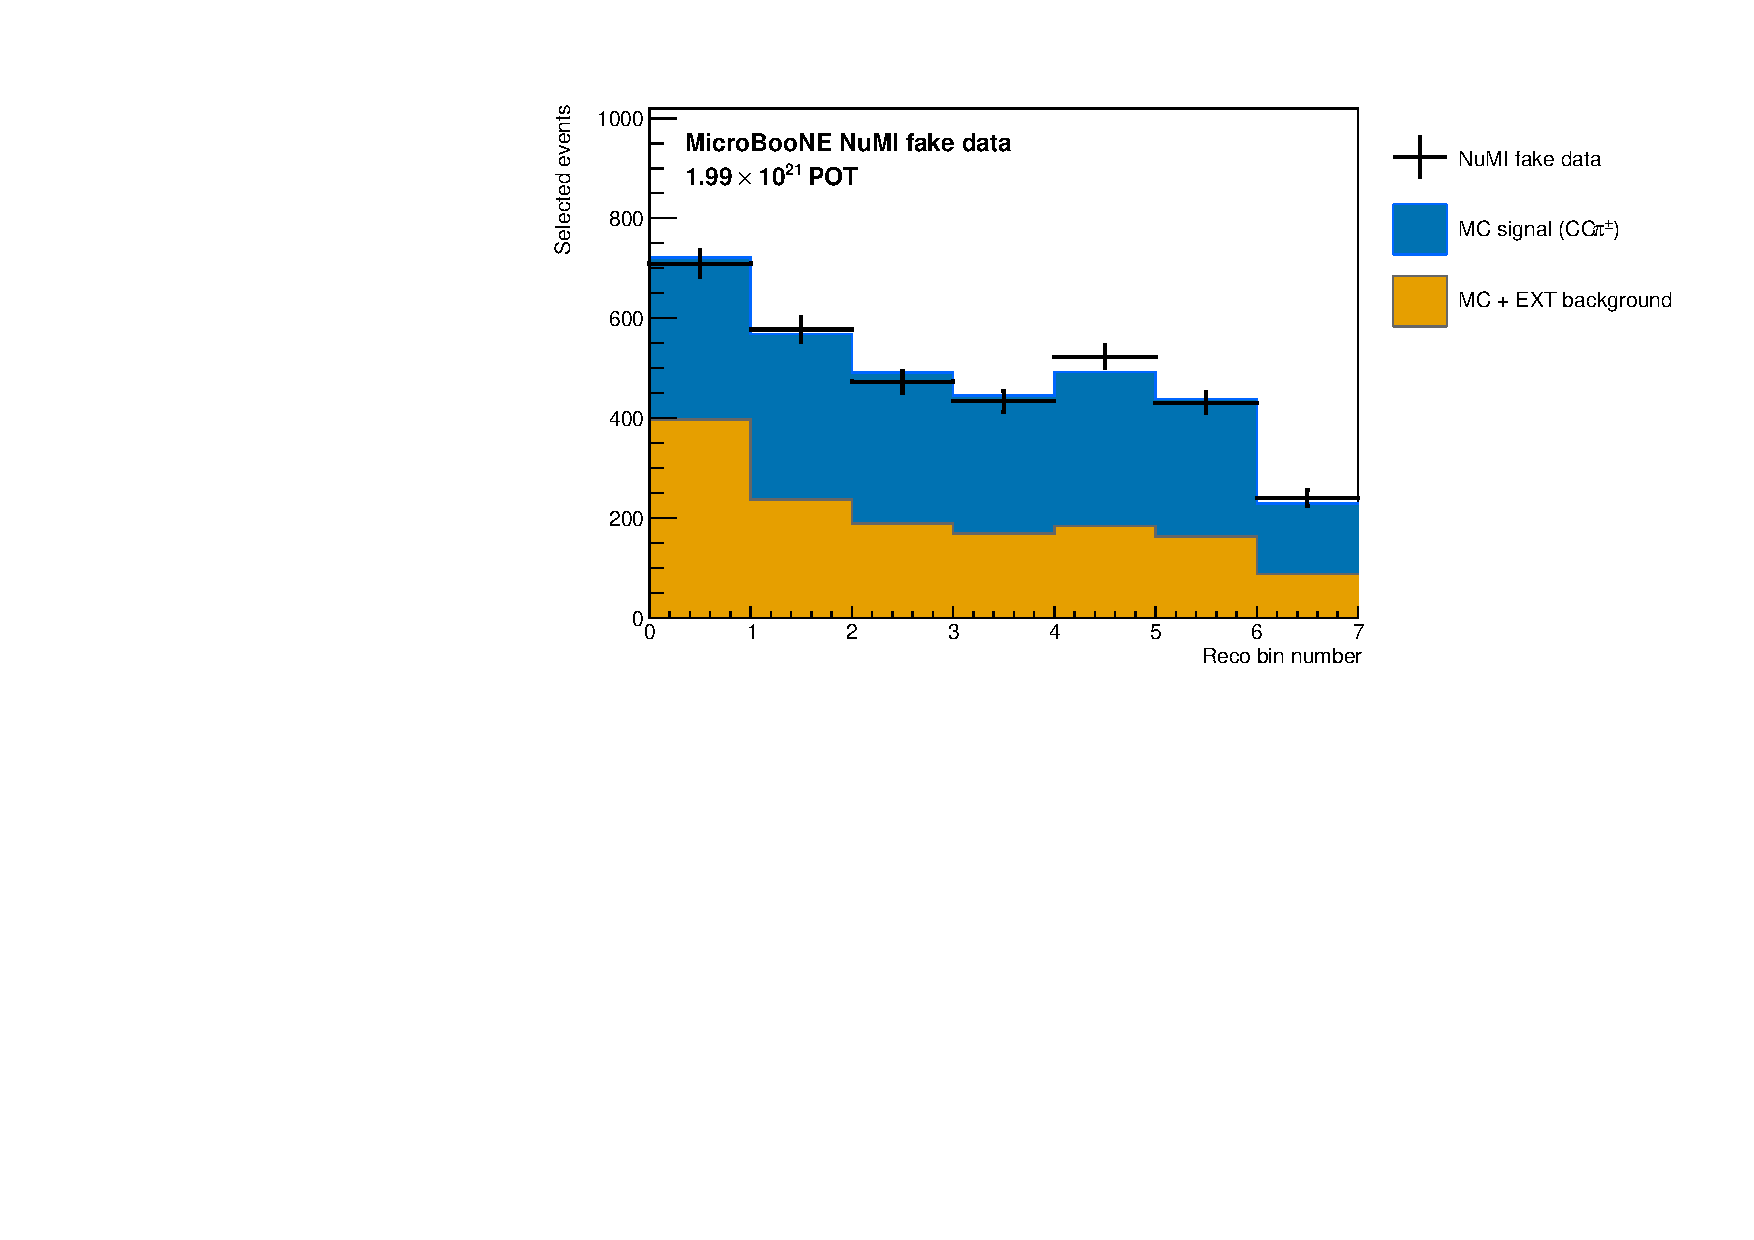
\includegraphics[width=\textwidth]{step1_reco_pmu_COMB}\caption{$p_\mu$}\end{subfigure}\hfill
  \begin{subfigure}[b]{0.32\textwidth}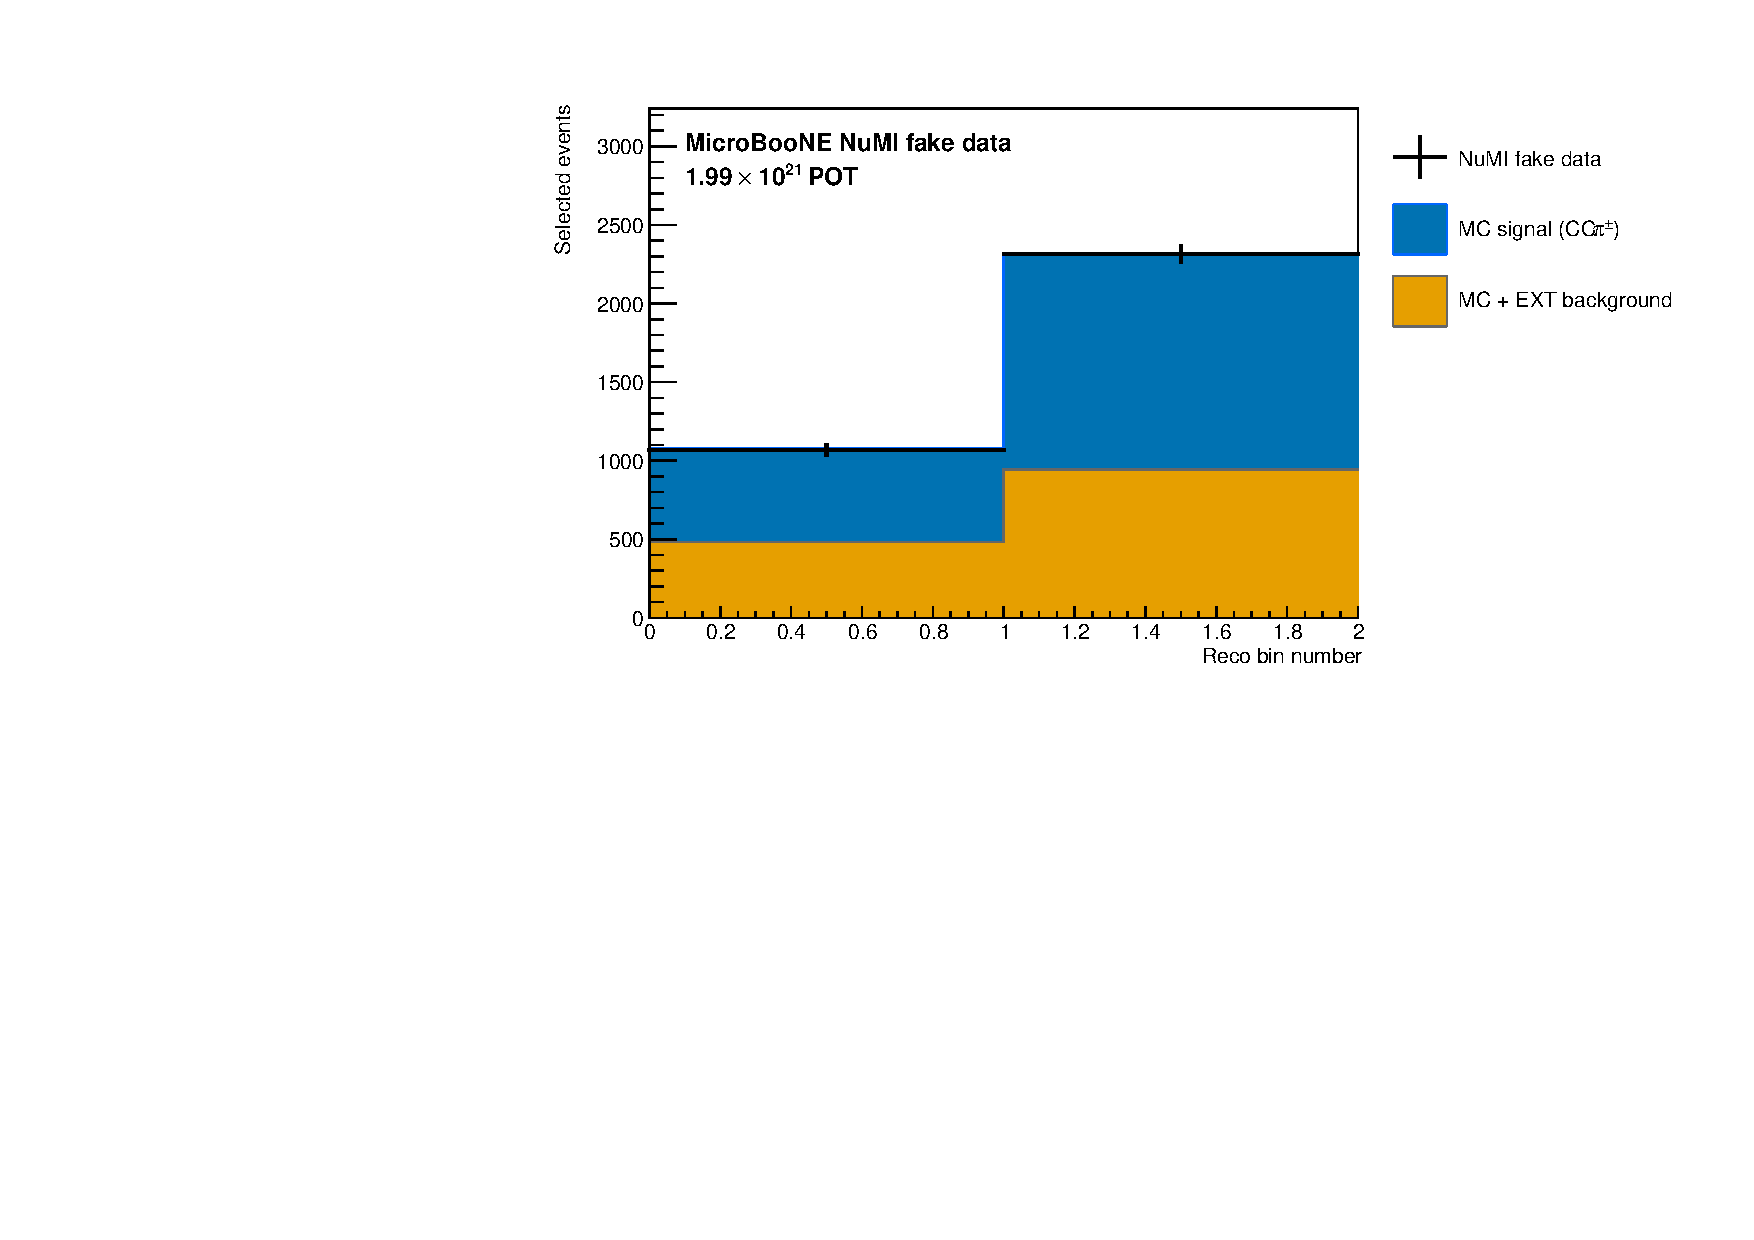
\includegraphics[width=\textwidth]{step1_reco_ppi_COMB}\caption{$p_\pi$}\end{subfigure}\hfill
  \begin{subfigure}[b]{0.32\textwidth}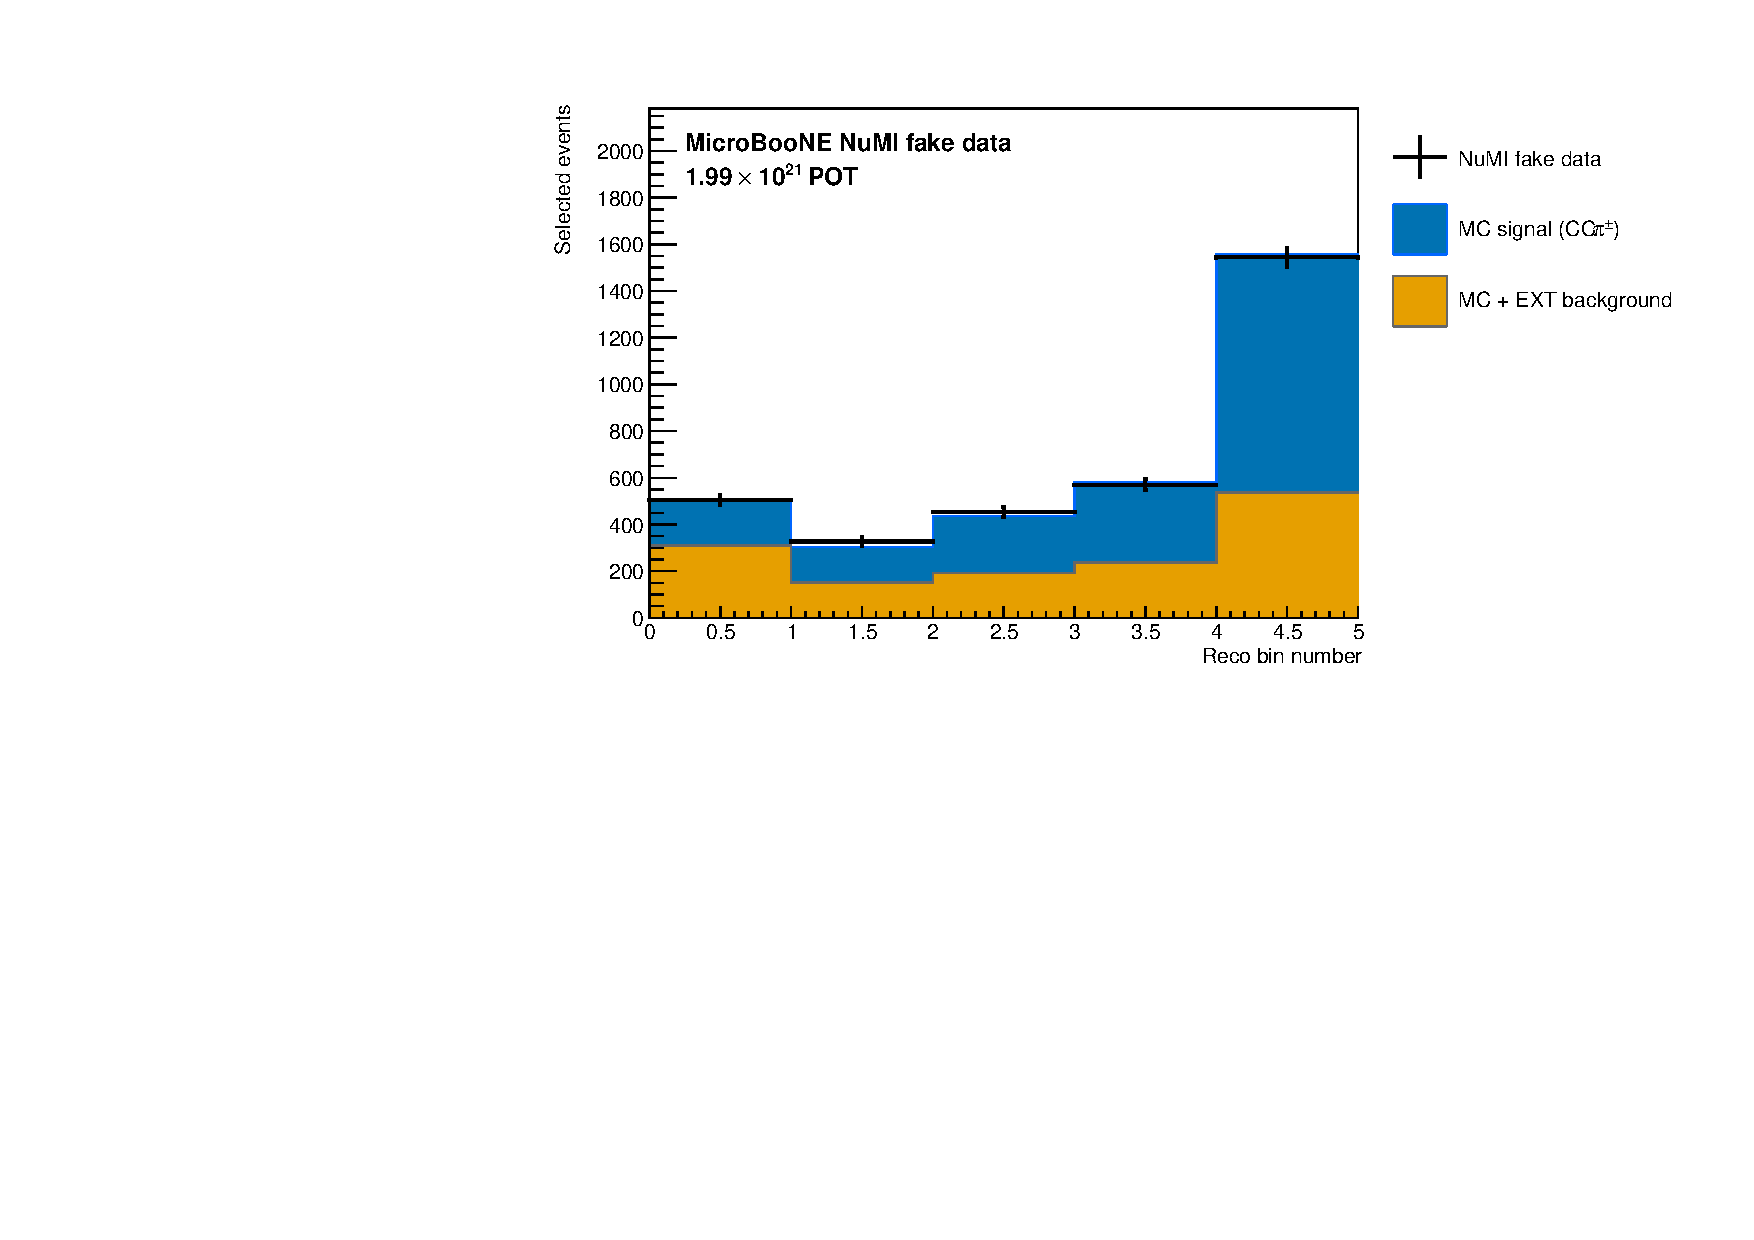
\includegraphics[width=\textwidth]{step1_reco_costhmu_COMB}\caption{$\cos\theta_\mu$}\end{subfigure}

  \vspace{3mm}
  \begin{subfigure}[b]{0.32\textwidth}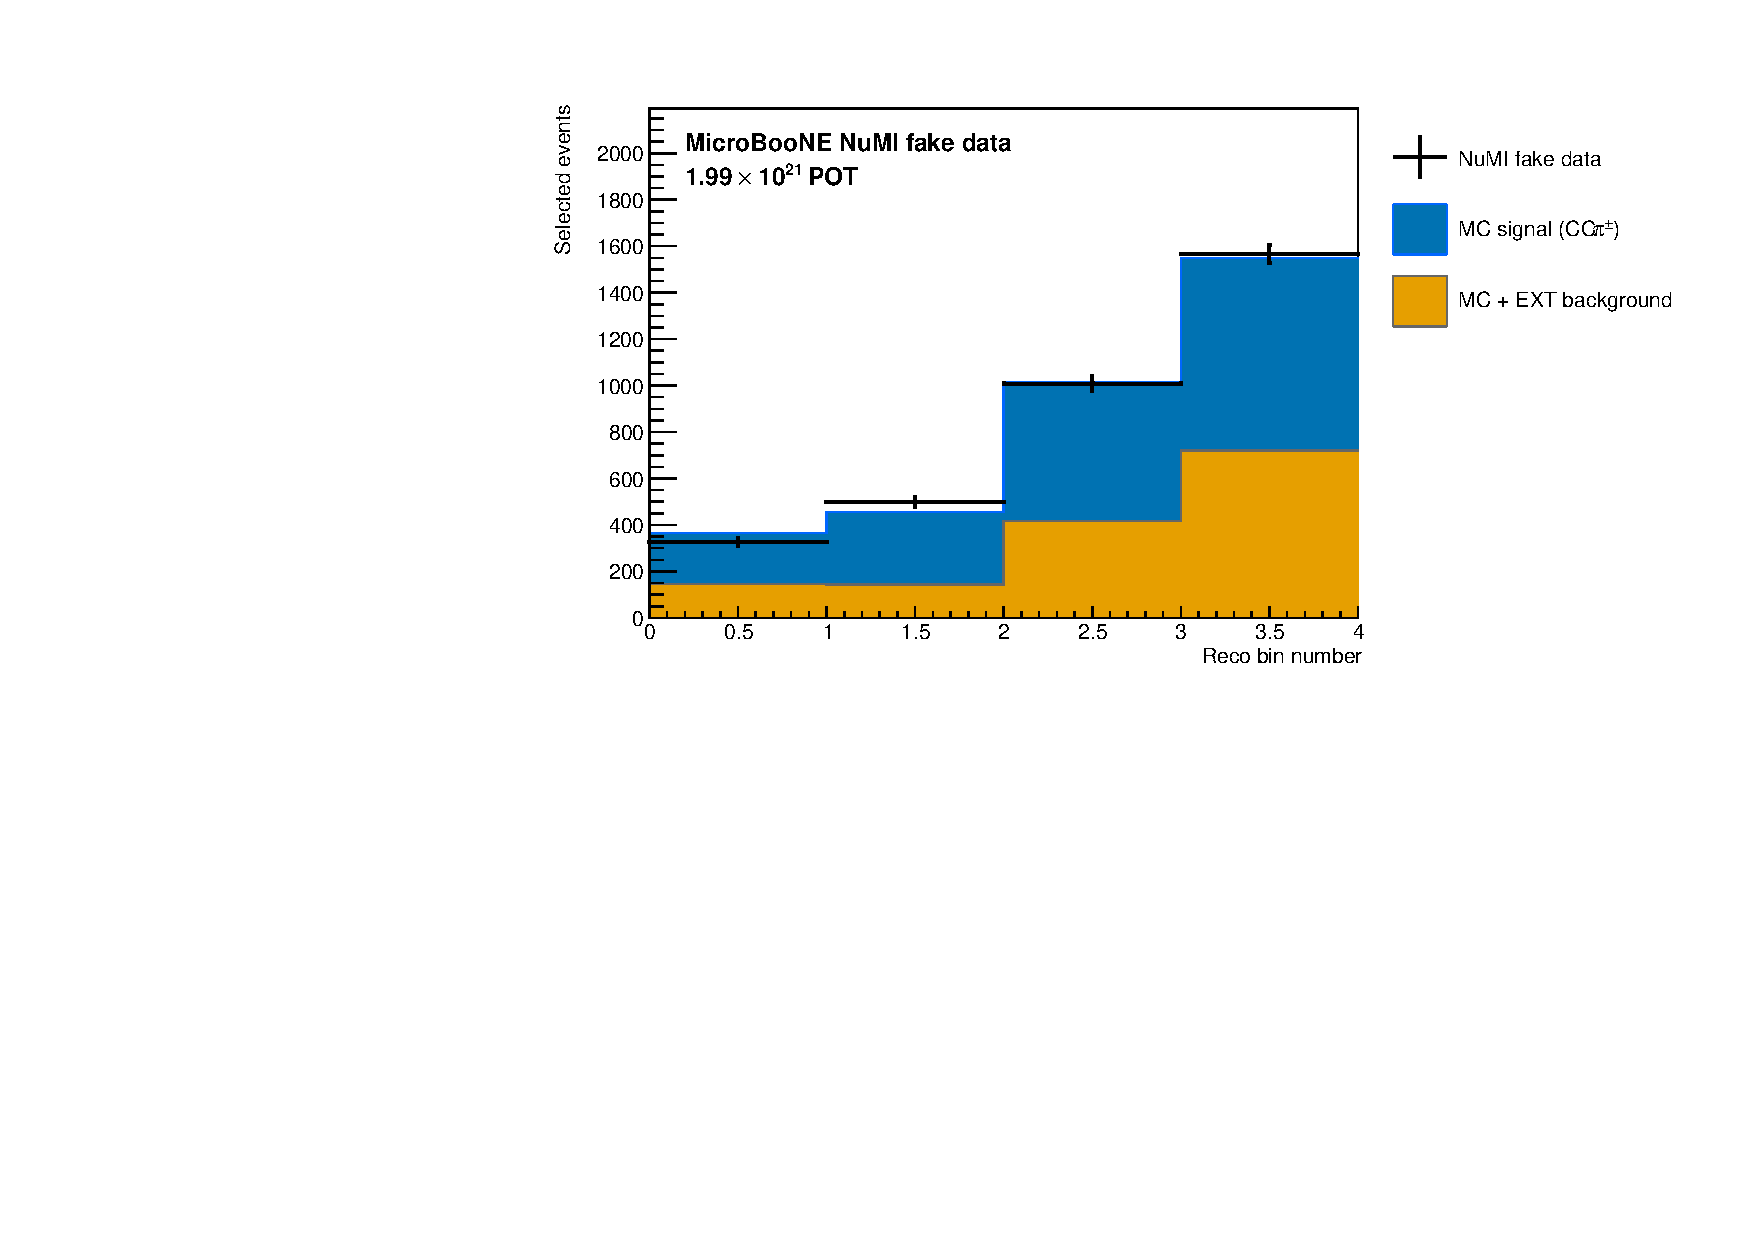
\includegraphics[width=\textwidth]{step1_reco_costhpi_COMB}\caption{$\cos\theta_\pi$}\end{subfigure}\hfill
  \begin{subfigure}[b]{0.32\textwidth}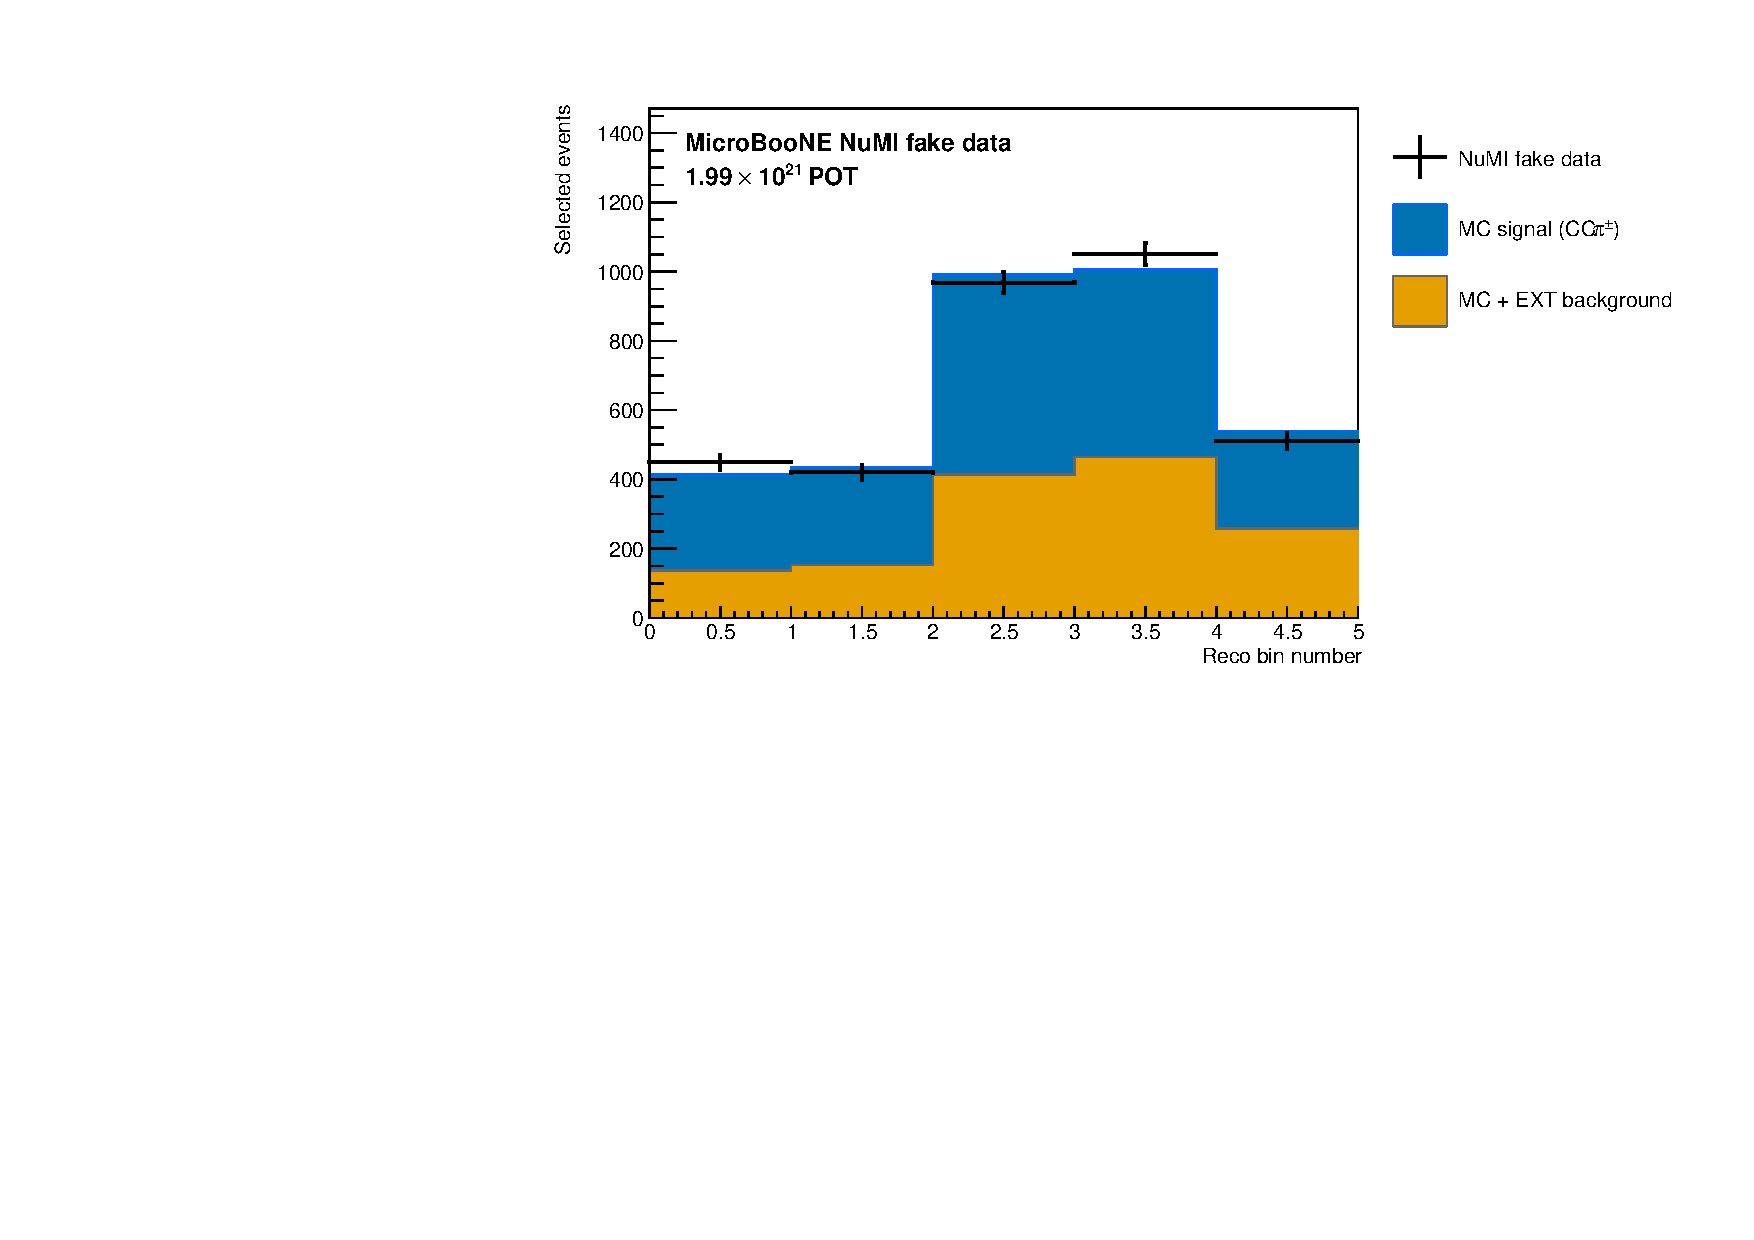
\includegraphics[width=\textwidth]{step1_reco_thmupi_COMB}\caption{$\theta_{\mu\pi}$}\end{subfigure}\hfill
  \begin{subfigure}[b]{0.32\textwidth}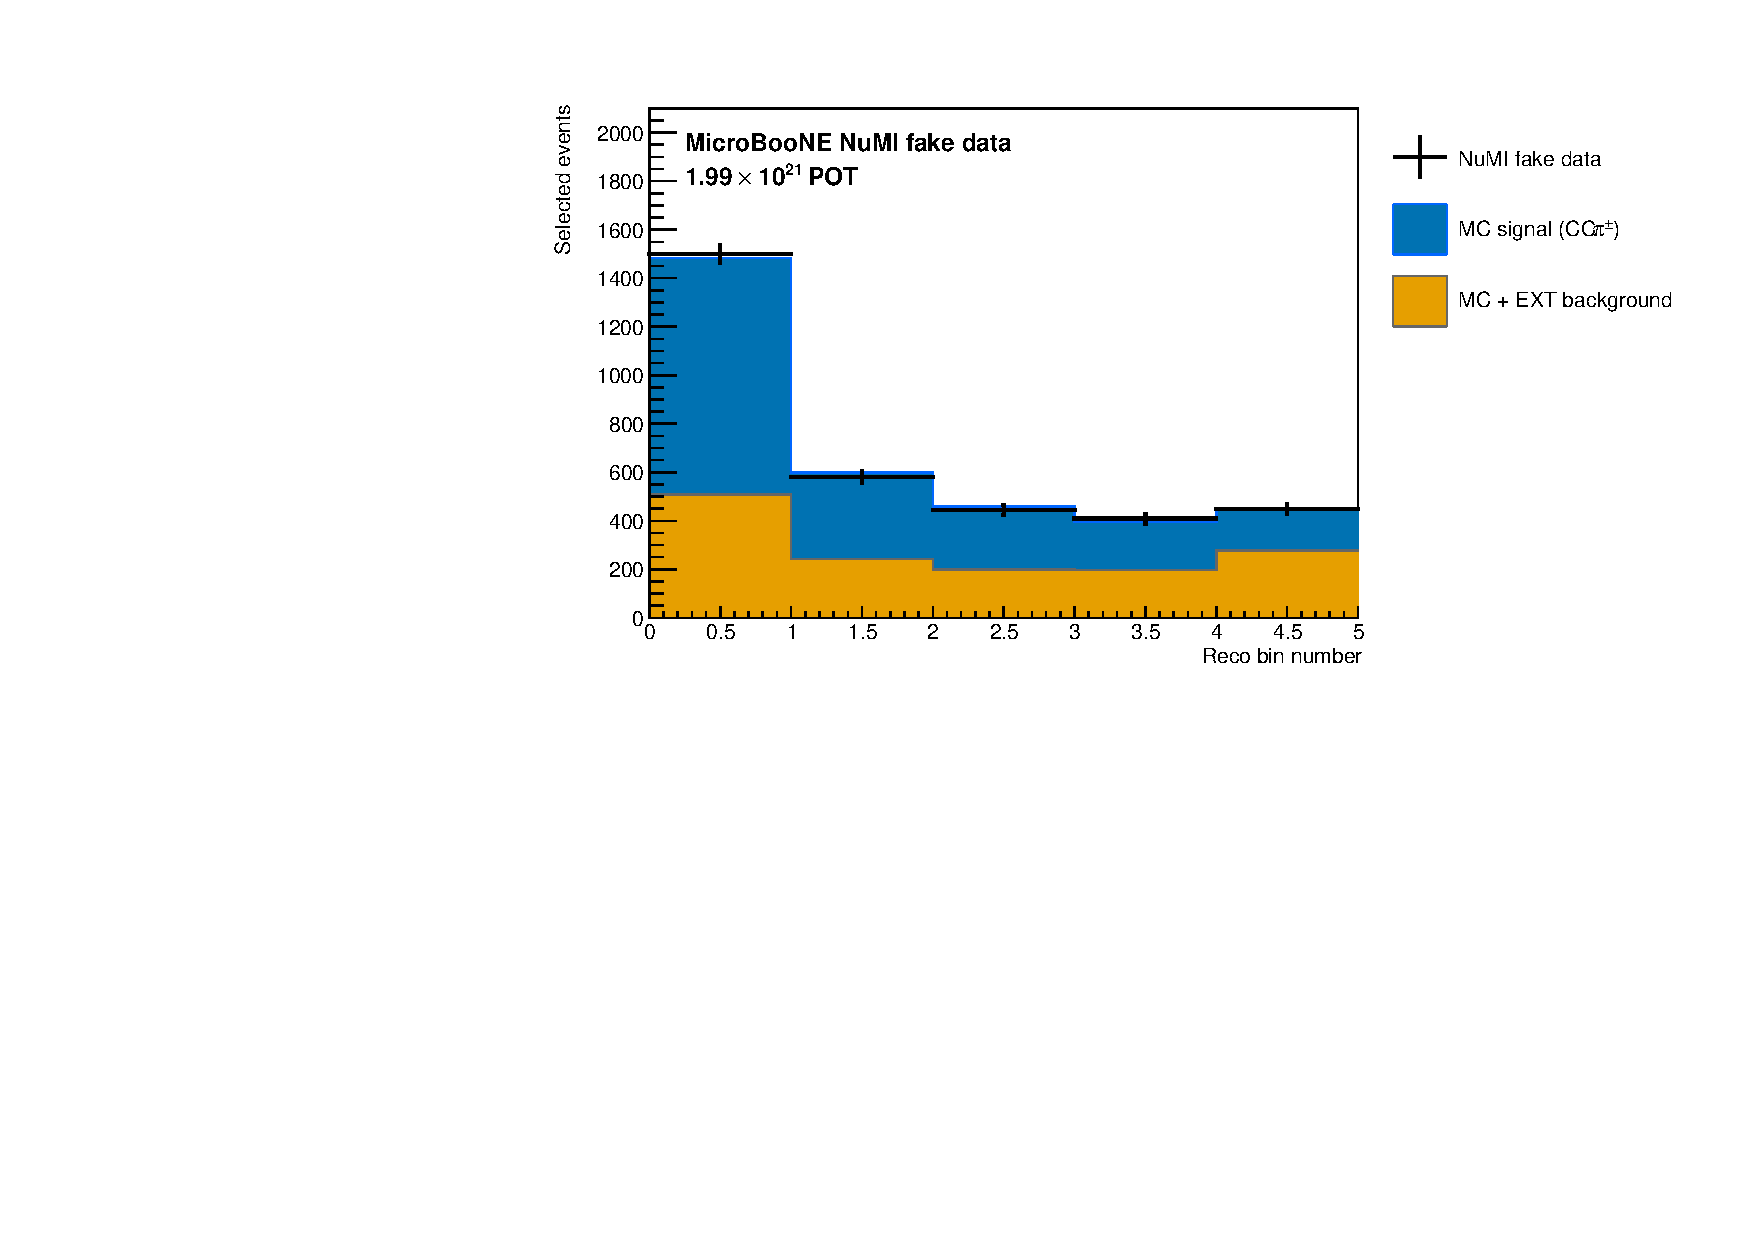
\includegraphics[width=\textwidth]{step1_reco_thetamu_COMB}\caption{$\theta_\mu$}\end{subfigure}
  \caption{Stage 1, combined: selected reconstructed spectra at the combined FHC$+$RHC exposure.}
  \label{fig:chain_reco_comb}
\end{figure}

\begin{figure}[H]
  \centering
  \begin{subfigure}[b]{0.32\textwidth}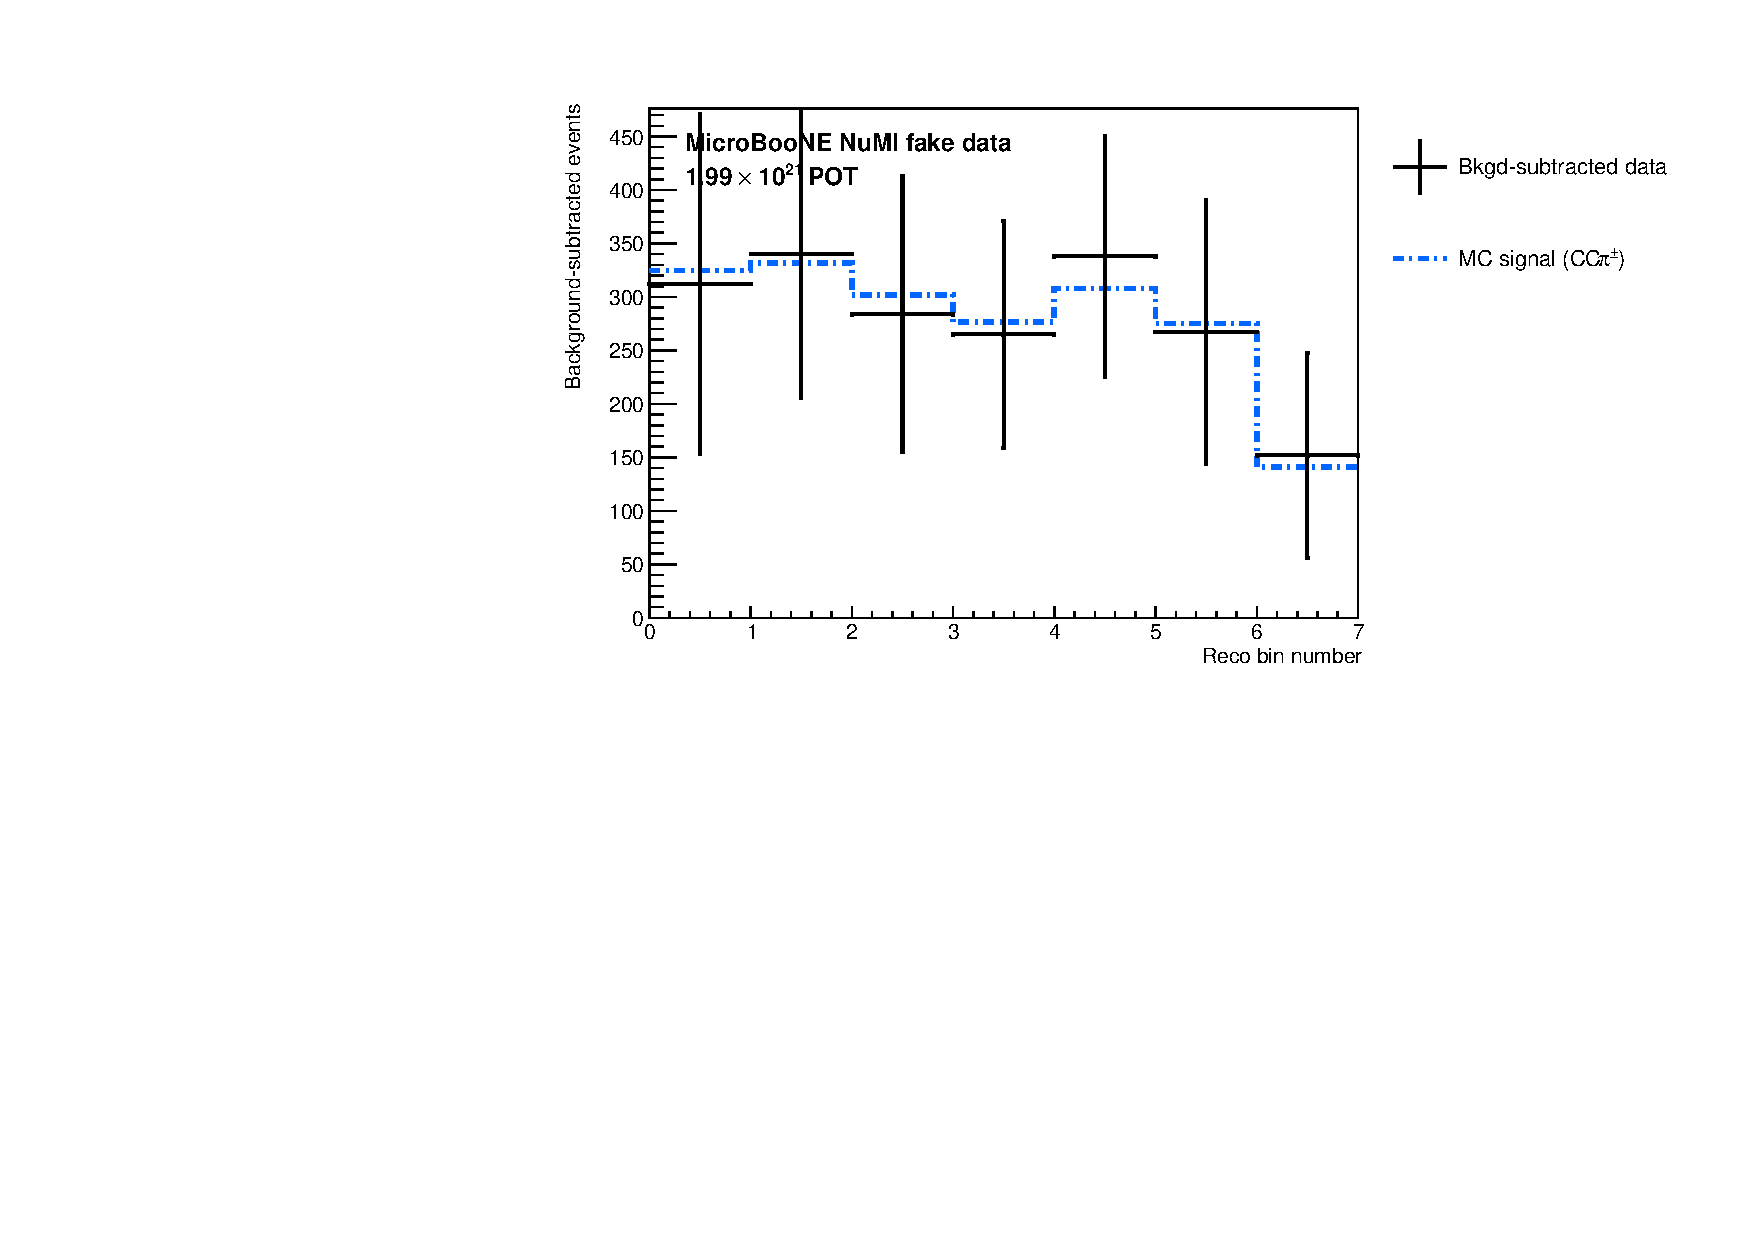
\includegraphics[width=\textwidth]{step2_bsub_pmu_COMB}\caption{$p_\mu$}\end{subfigure}\hfill
  \begin{subfigure}[b]{0.32\textwidth}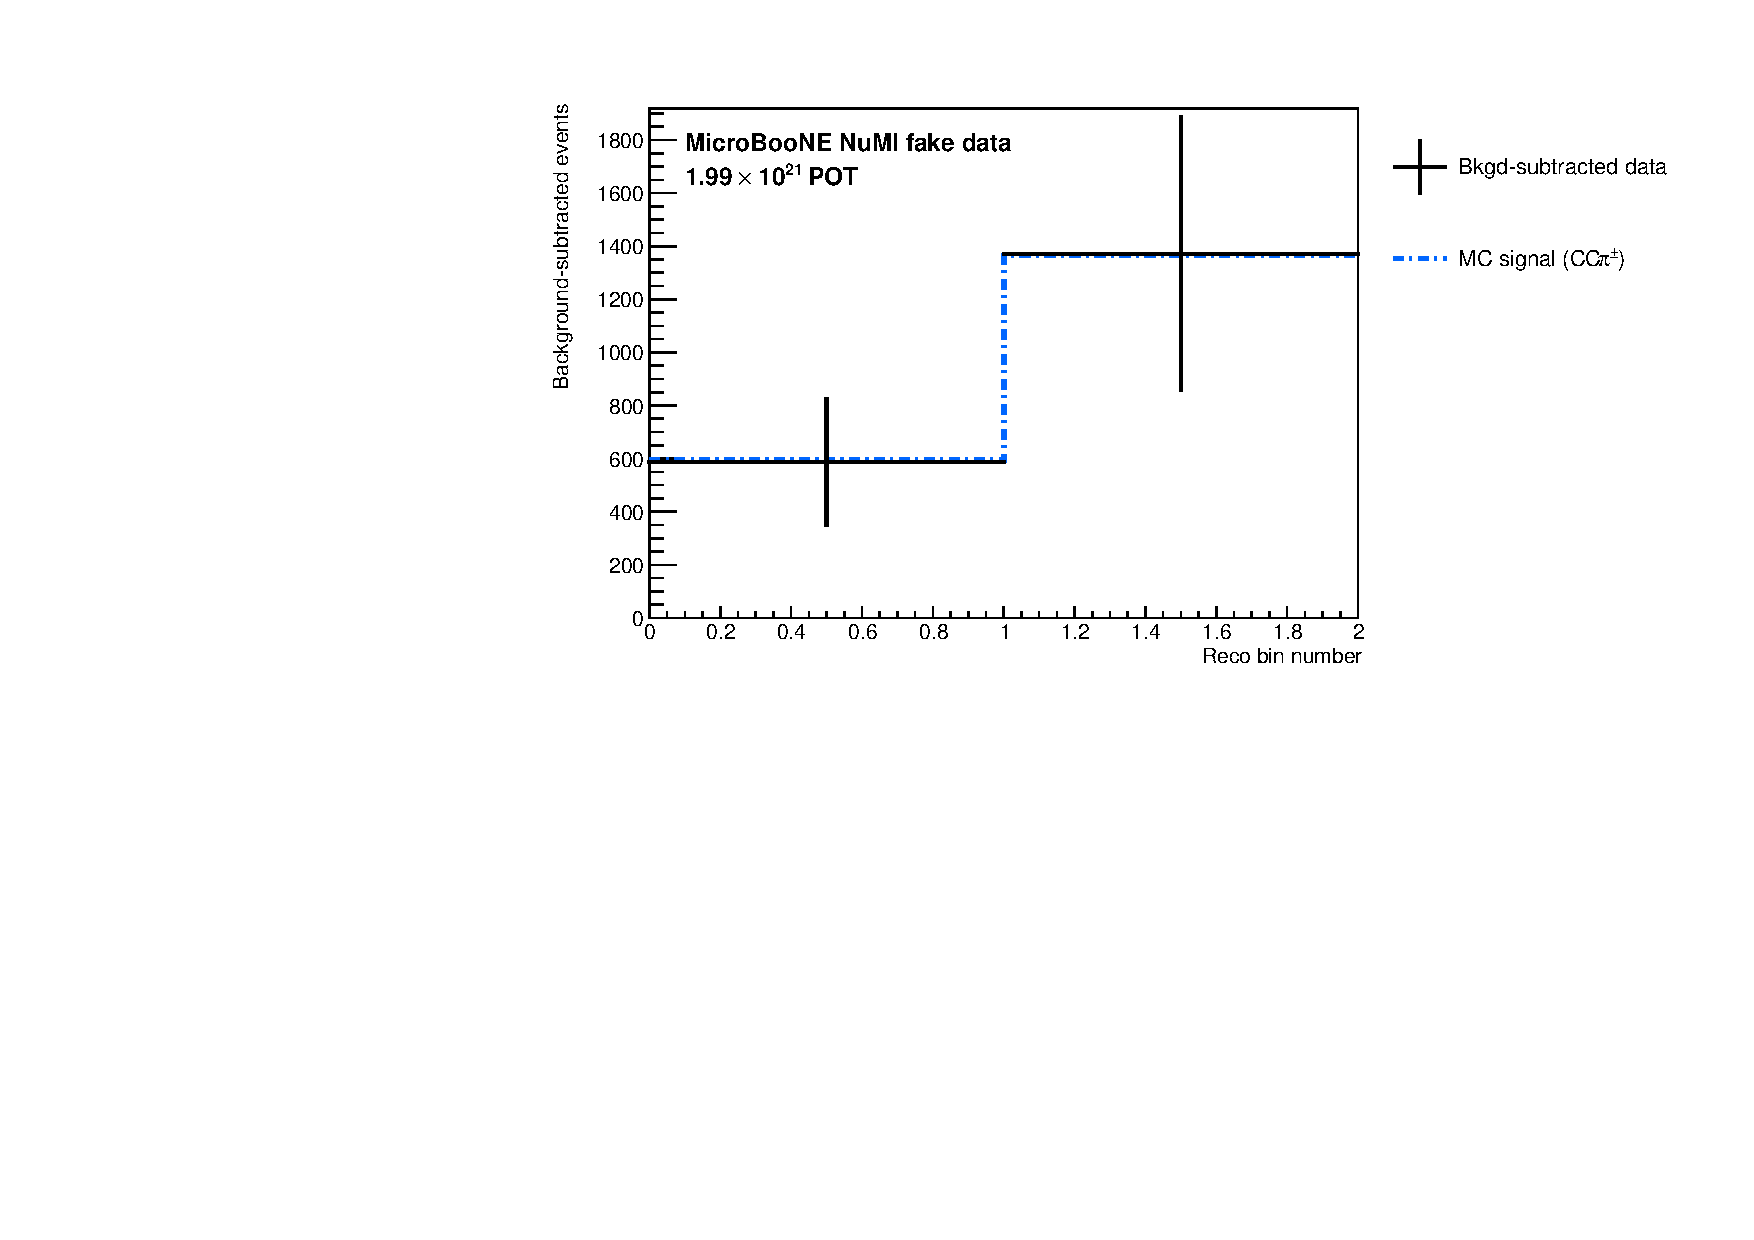
\includegraphics[width=\textwidth]{step2_bsub_ppi_COMB}\caption{$p_\pi$}\end{subfigure}\hfill
  \begin{subfigure}[b]{0.32\textwidth}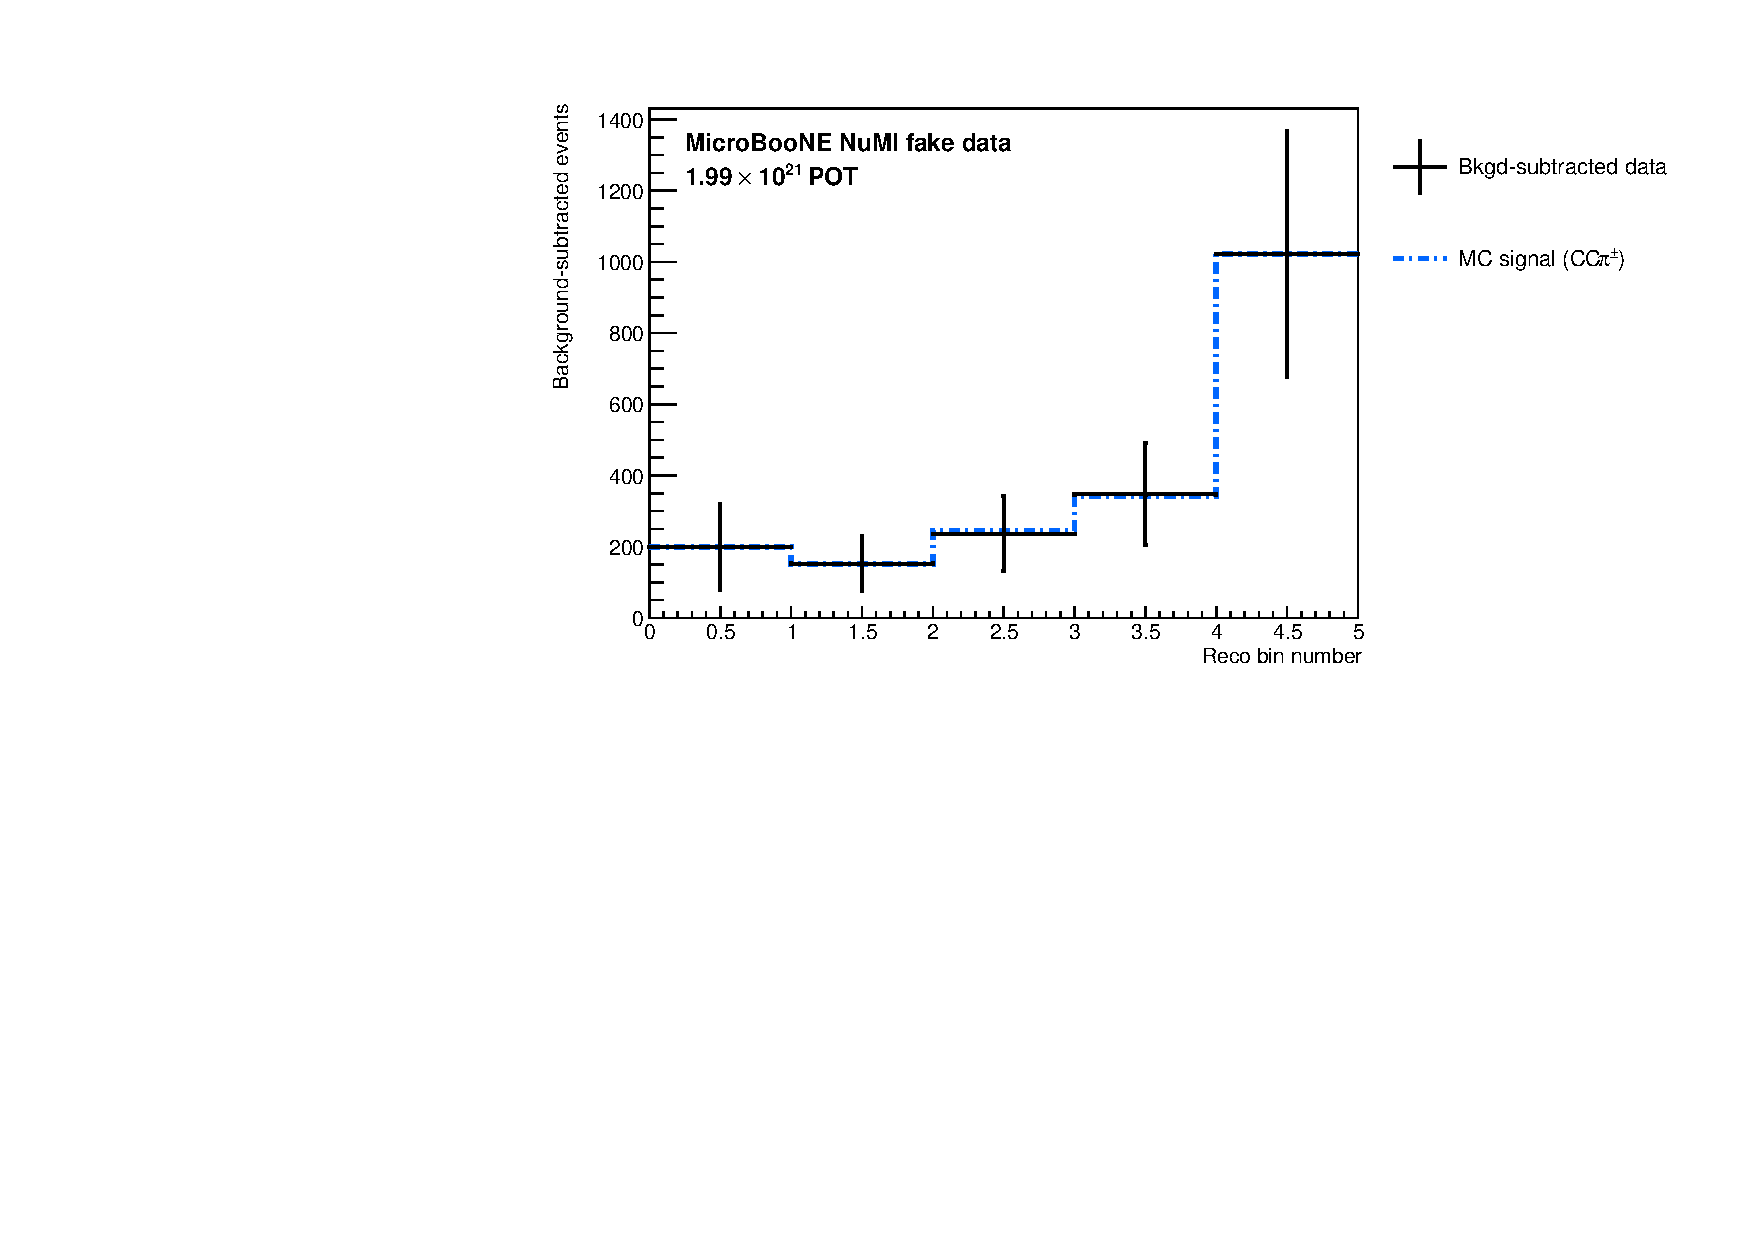
\includegraphics[width=\textwidth]{step2_bsub_costhmu_COMB}\caption{$\cos\theta_\mu$}\end{subfigure}

  \vspace{3mm}
  \begin{subfigure}[b]{0.32\textwidth}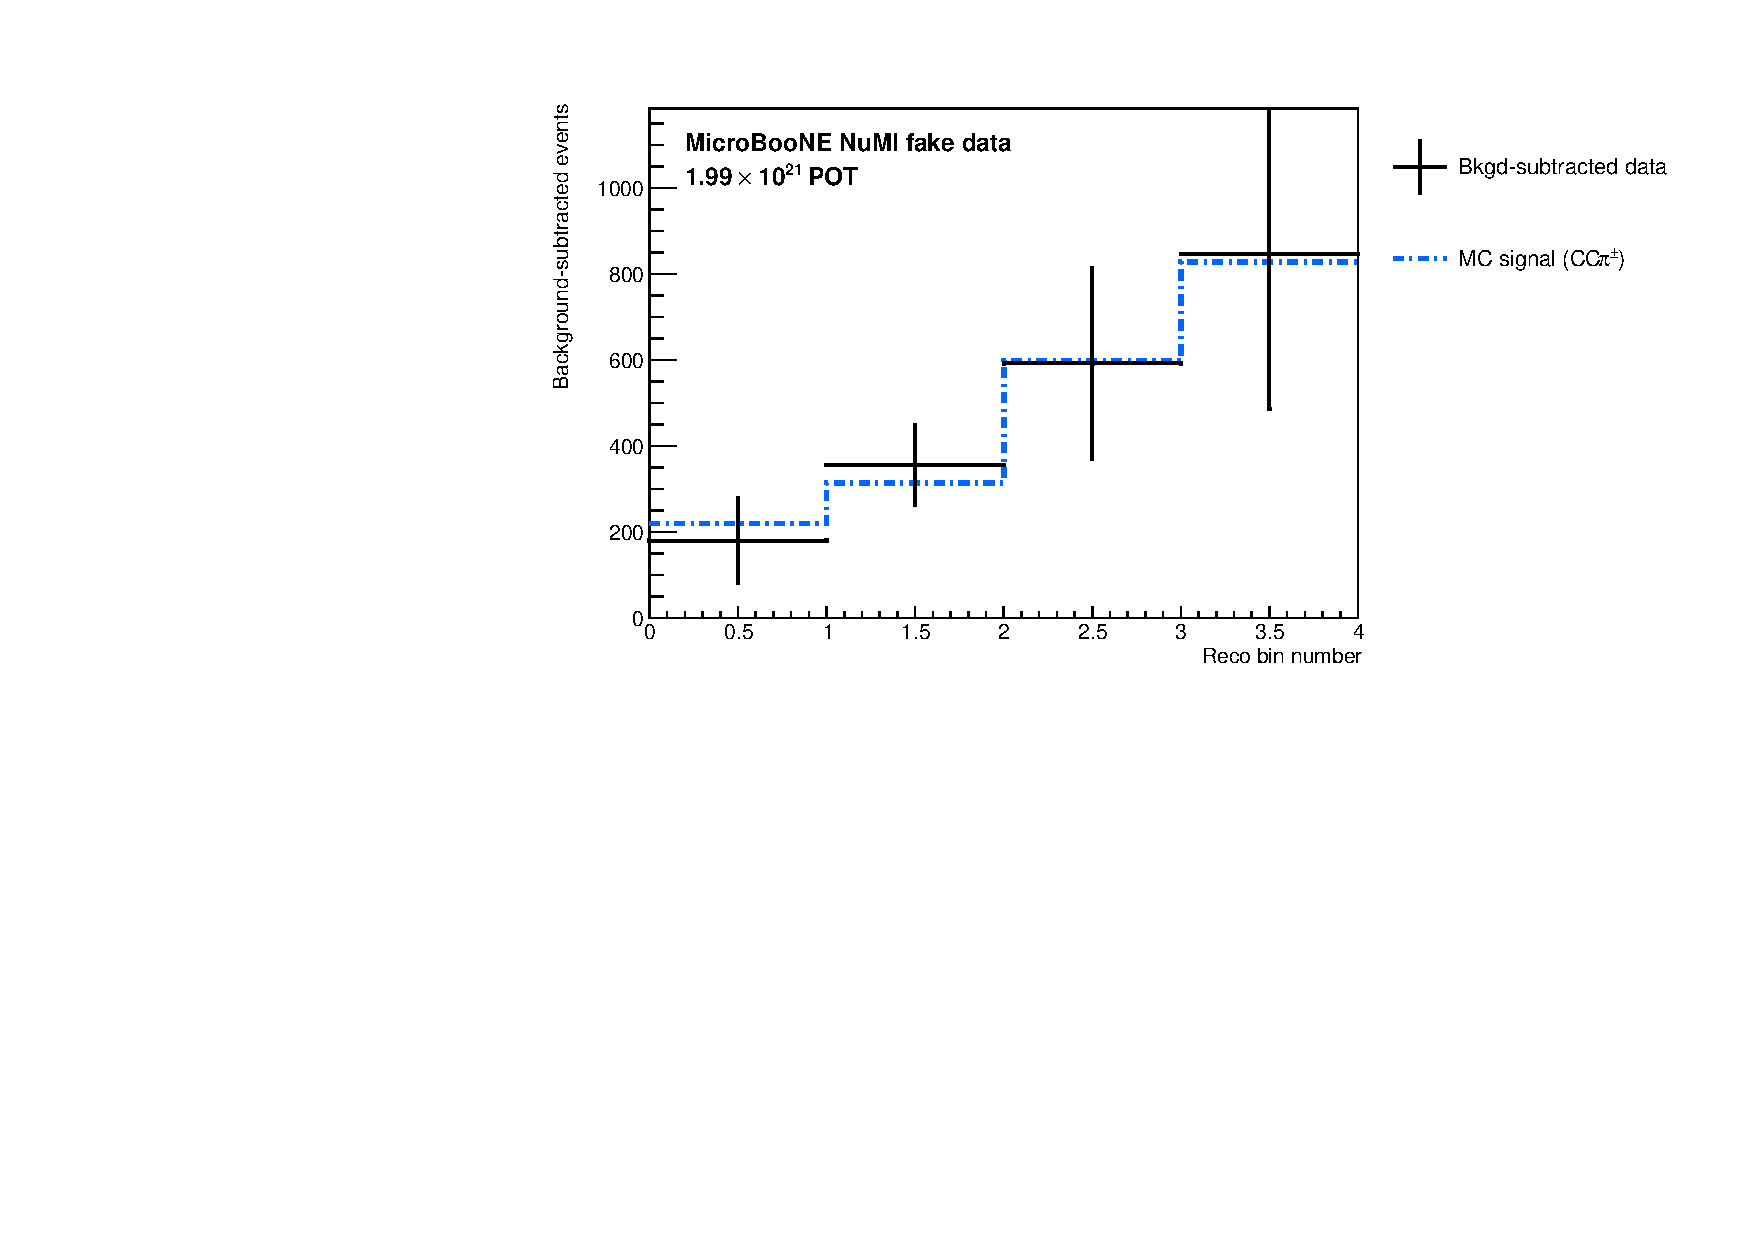
\includegraphics[width=\textwidth]{step2_bsub_costhpi_COMB}\caption{$\cos\theta_\pi$}\end{subfigure}\hfill
  \begin{subfigure}[b]{0.32\textwidth}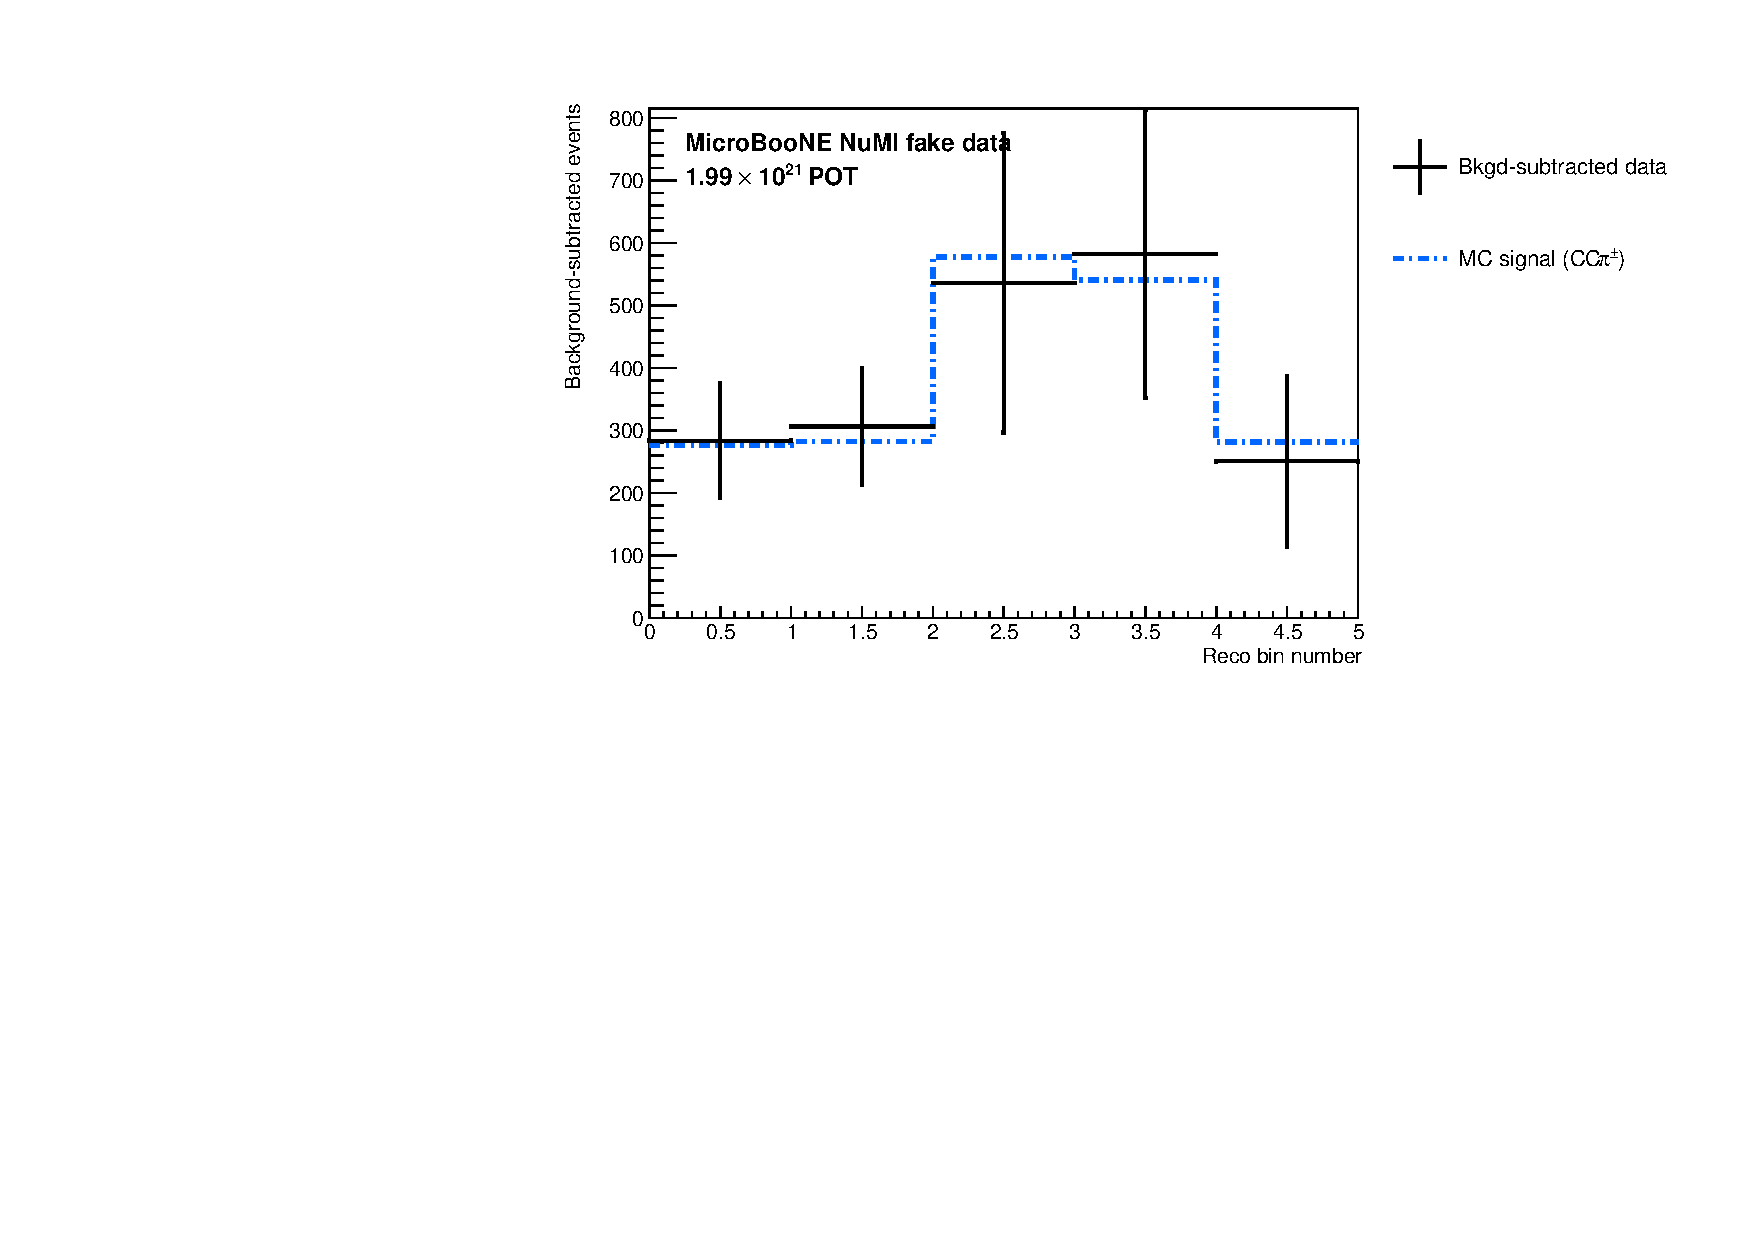
\includegraphics[width=\textwidth]{step2_bsub_thmupi_COMB}\caption{$\theta_{\mu\pi}$}\end{subfigure}\hfill
  \begin{subfigure}[b]{0.32\textwidth}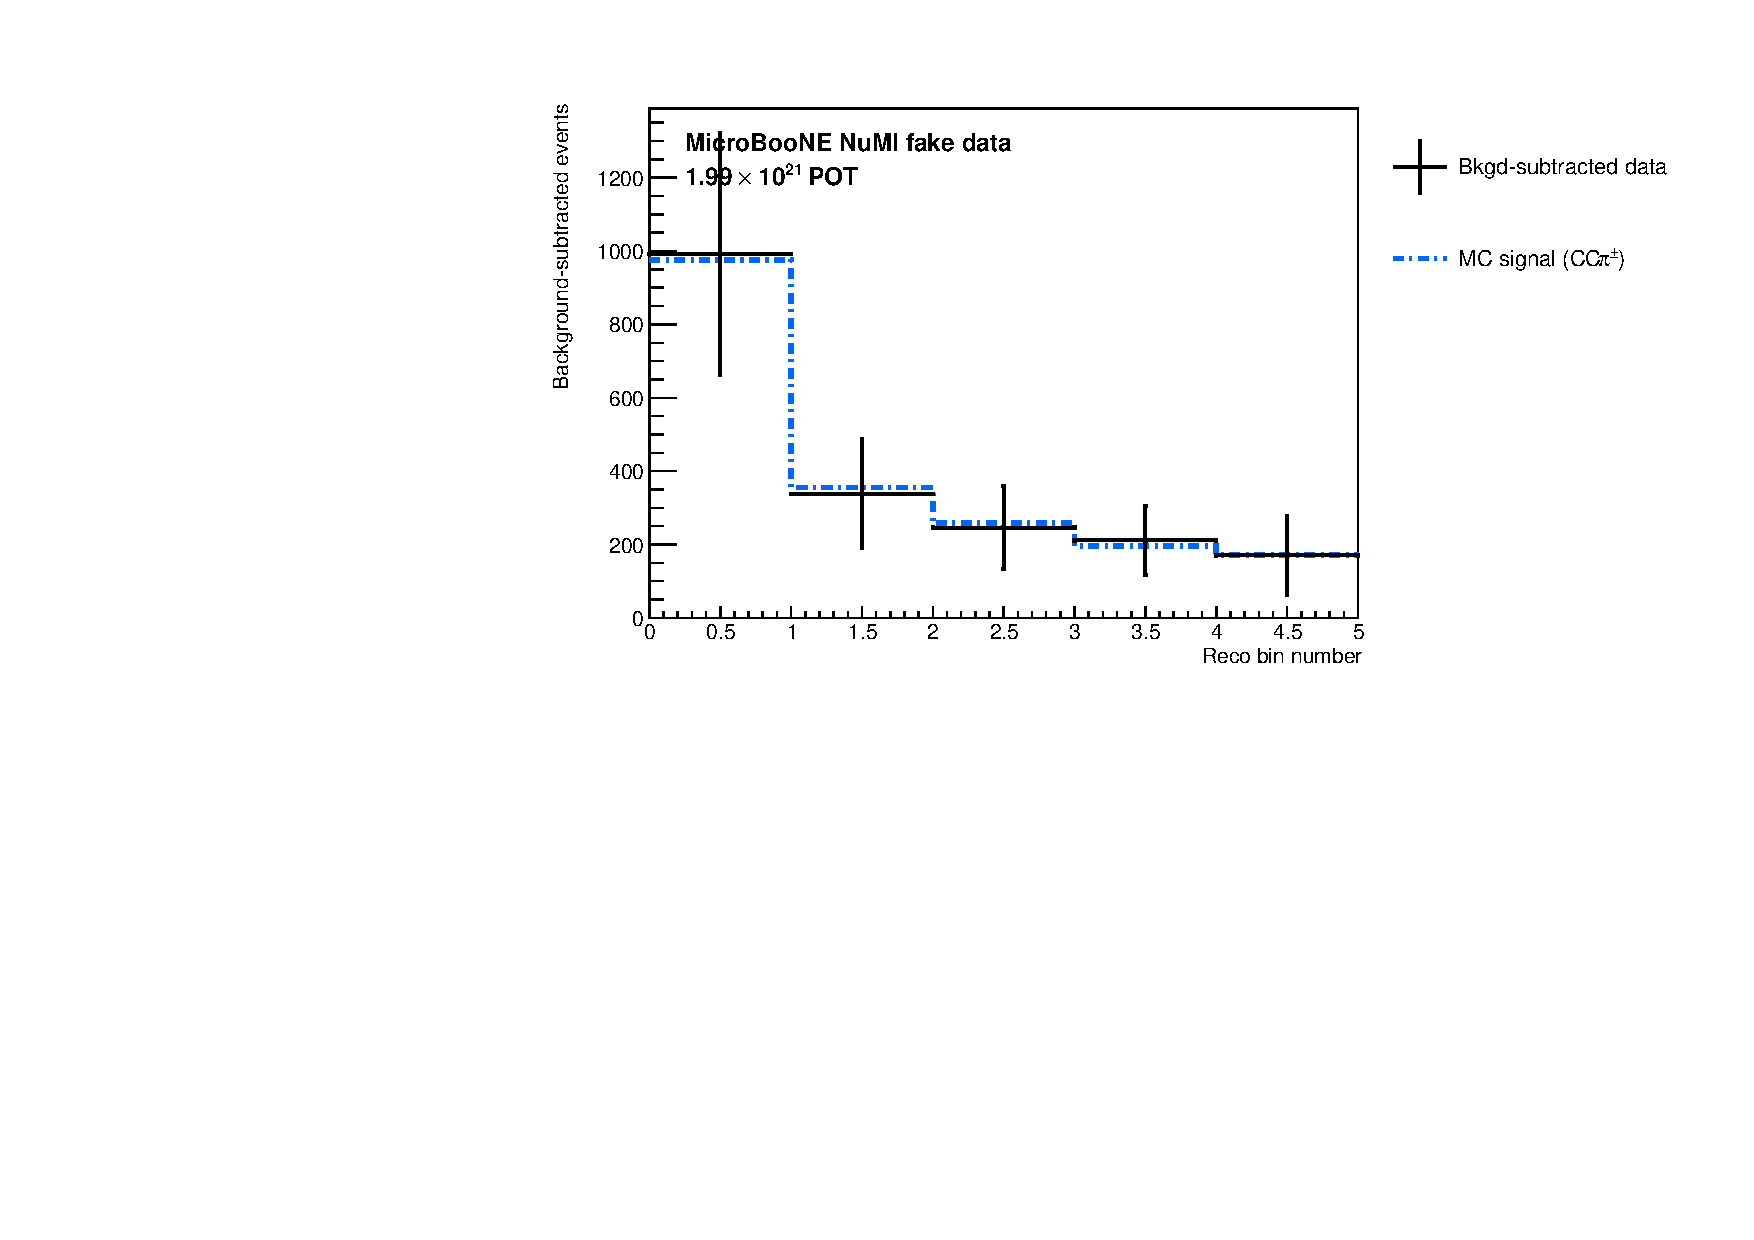
\includegraphics[width=\textwidth]{step2_bsub_thetamu_COMB}\caption{$\theta_\mu$}\end{subfigure}
  \caption{Stage 2, combined: background-subtracted data compared with the central-value MC signal.}
  \label{fig:chain_bsub_comb}
\end{figure}

\subsection{The rejected five-bin $p_\pi$ response}
\label{sec:supp_resp5}

\begin{figure}[H]
  \centering
  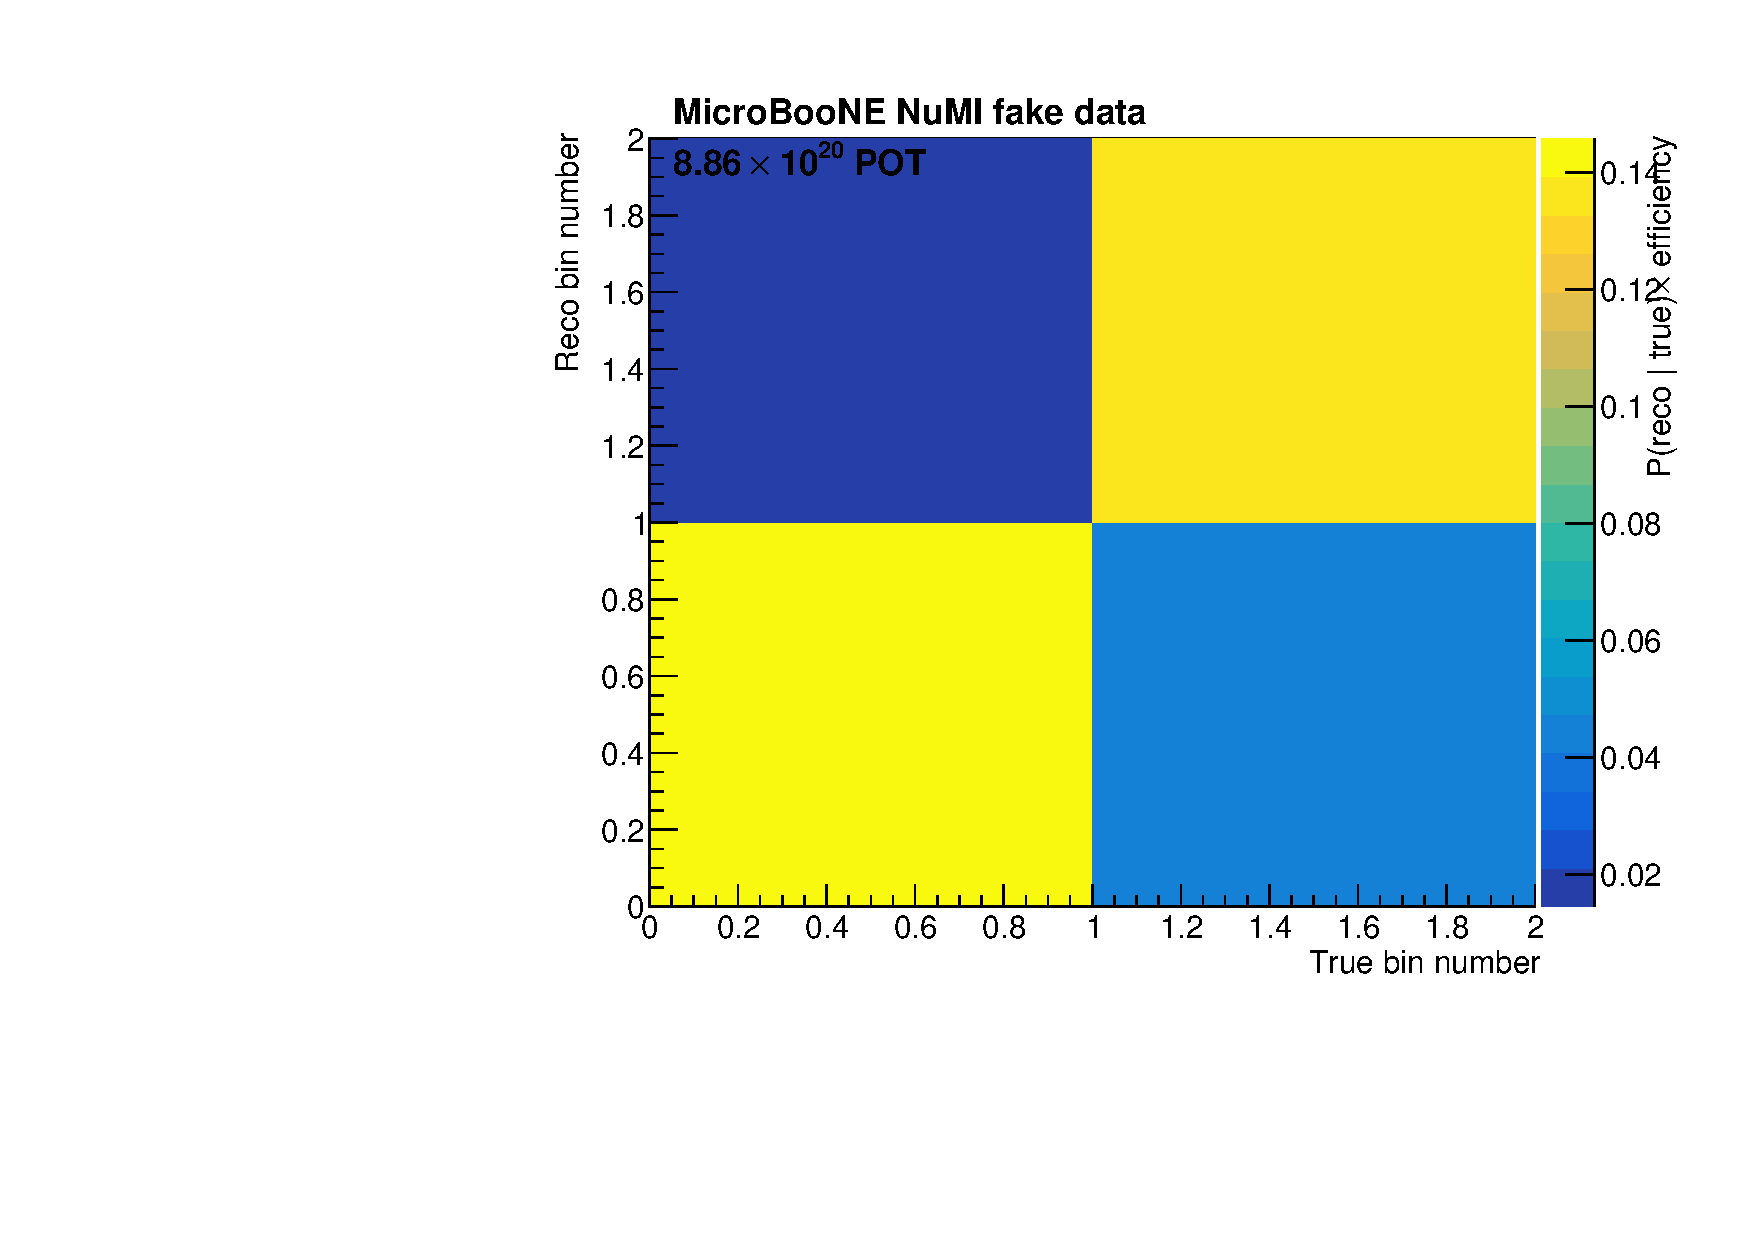
\includegraphics[width=0.6\textwidth]{fw_resp_ppi}
  \caption{Smearceptance matrix of the rejected five-bin $p_\pi$ scheme (FHC): reconstructed
    events pile into the lowest bin from every true bin, the diagnostic that motivated the
    two-bin scheme of \S\ref{sec:ppi2bin_adopted}; the released two-bin response is in the
    analysis note.}
  \label{fig:resp_ppi5}
\end{figure}

\subsection{$A_C$ row sums of every released extraction}
\label{sec:supp_ac}

Row sums of the released additional-smearing matrices, inclusive and proton-tagged, and
the two matrices with a negative row.

\begin{center}
\small
\begin{tabular}{lccc}
\toprule
Observable & FHC & RHC & combined \\
\midrule
\multicolumn{4}{l}{\emph{Inclusive}}\\
\midrule
$p_\mu$ & $0.66$--$0.91$ & $0.58$--$0.99$ & $0.68$--$1.01$ \\
$p_\pi$ (2-bin) & $0.35$--$0.54$ & $0.40$--$0.51$ & $0.29$--$0.54$ \\
$\cos\theta_\mu$ & $0.17$--$0.39$ & $0.05$--$0.45$ & $0.09$--$0.43$ \\
$\cos\theta_\pi$ & $0.68$--$0.77$ & $0.70$--$0.84$ & $0.71$--$0.83$ \\
$\theta_{\mu\pi}$ & $0.52$--$1.03$ & $0.58$--$1.15$ & $0.63$--$1.21$ \\
$\theta_\mu$ & $0.58$--$0.78$ & $0.22$--$1.16$ & $0.53$--$0.67$ \\
\midrule
\multicolumn{4}{l}{\emph{Proton-tagged}}\\
\midrule
$p_\mu$ & $0.46$--$1.00$ & $0.55$--$0.89$ & $0.65$--$0.96$ \\
$p_\pi$ (2-bin) & $0.34$--$0.84$ & $0.41$--$0.45$ & $0.47$--$0.48$ \\
$\cos\theta_\mu$ & $0.61$--$0.70$ & $-0.08$--$0.57$ & $0.28$--$0.46$ \\
$\cos\theta_\pi$ & $0.66$--$0.77$ & $0.62$--$0.77$ & $0.65$--$0.76$ \\
$\theta_{\mu\pi}$ & $0.37$--$0.87$ & $0.31$--$0.75$ & $0.35$--$0.78$ \\
$W_{\pi p}$ & $0.45$--$1.22$ & $-0.14$--$1.26$ & $0.32$--$1.24$ \\
$W_{\rm had}$ & $0.54$--$0.81$ & $0.30$--$0.86$ & $0.18$--$0.87$ \\
$\delta p_T$ & $0.54$--$0.86$ & $0.45$--$0.82$ & $0.47$--$0.87$ \\
$\delta\phi_T$ & $0.65$--$0.78$ & $0.53$--$0.72$ & $0.28$--$0.67$ \\
$\delta\alpha_T$ & $0.59$--$0.98$ & $0.57$--$0.93$ & $0.60$--$0.96$ \\
$p_n$ & $0.71$--$0.86$ & $0.61$--$0.82$ & $0.59$--$0.86$ \\
\bottomrule
\end{tabular}
\end{center}

Three features matter for interpretation.

The suppression is large: inclusive $\cos\theta_\mu$ has a row sum as low as $0.05$ in
RHC, a strong suppression of that output mode for a flat input.  It also differs strongly between observables, which is
precisely why the integrated cross section obtained by summing a differential result
varies from observable to observable while the underlying physical total cannot.  The
D'Agostini cross-check, whose integral is flat across observables, is what establishes
that this spread is the smearing rather than a physical or acceptance effect.

Two extractions have \emph{negative} row sums, and the pattern identifies their cause.
In $W_{\pi p}$ the top row carries negative off-diagonal terms in \emph{all three}
configurations (summing to $-0.14$ FHC, $-0.30$ combined, $-0.61$ RHC against diagonals of
$0.73$, $0.62$ and $0.47$); only RHC tips negative overall (row sum $-0.14$), because its
diagonal element is the smallest of the three.  The same happens in the first
$\cos\theta_\mu$ bin of the proton-tagged RHC sample, whose diagonal is $0.079$ against
off-diagonal terms summing to $-0.16$ (row sum $-0.08$).

So this is not an RHC-specific defect but the regularisation pushing back against the
least-determined bin of each observable --- for $W_{\pi p}$, the same top bin that is only
$2\%$ diagonal in the six-bin response and that already led to withdrawing the
differential shape.  A negative row is not forbidden, since $A_C$ is a regularisation
operator rather than a probability matrix, but a prediction smeared through one is being
told that raising the truth in that bin \emph{lowers} the measured content, which is a
statement about the regularisation and not about the detector.  Treat those two rows with
corresponding caution.


\subsection{Ensemble study: reference construction and full-covariance pulls}
\label{sec:supp_ensemble}

\paragraph{Ensemble coverage: are the uncertainties the right size?}
\label{par:ensemble}
The closure test above uses a single throw.  It can show that the extraction reproduces
its input, but a single residual has no width, so it cannot say whether the quoted
uncertainty is correctly sized.  To answer that, thirty-two statistically independent
Poisson realisations of the FHC data were each put through the \emph{whole} chain ---
thrown, universes rebuilt from that throw, unfolded --- and the per-bin pull
\[
  p_i \;=\; \frac{\hat{x}_i - \left(A_C\,x_{\rm CV}\right)_i}{\sigma_i}
\]
formed against the fixed central-value truth smeared by that member's own $A_C$.  (The
per-throw \emph{fake-data} truth is not a valid reference: it follows the Poisson draw, so
numerator and reference fluctuate together and the width comes out too small.)

Three extractions were run on the current release, each with the same 32 throws
(with the weight rule of \noteref{Eq.}{eq:safeweight}),
chosen to bracket the
conditioning: the well-behaved $p_\mu$; $\cos\theta_\mu$, whose $A_C$ row sums fall as
low as $0.17$ in FHC ($0.050$ in RHC) so that the regularisation removes up to $83\%$
($95\%$) of a bin's normalisation;
and the one-bin total, which has no regularisation at all. If the uncertainties were
mis-sized anywhere, the second is where it would show; if the extraction carried a bias
independent of the regularisation, the third is where it would show.

\begin{center}
\small
\begin{tabular}{lccc}
\toprule
Reference covariance & pull mean & pull width & 68\% / 95\% coverage \\
\midrule
\multicolumn{4}{l}{\emph{statistical only}}\\
$d\sigma/dp_\mu$        & $-0.05$ & $1.08$ & $62.1\%$ / $92.0\%$ \\
$d\sigma/d\cos\theta_\mu$ & $-0.18$ & $0.97$ & $71.2\%$ / $93.1\%$ \\
one-bin total           & $-0.25$ & $1.02$ & $62.5\%$ / $93.8\%$ \\
\midrule
\multicolumn{4}{l}{\emph{full}}\\
$d\sigma/dp_\mu$        & $-0.01$ & $0.35$ & $99.1\%$ / $100\%$ \\
$d\sigma/d\cos\theta_\mu$ & $-0.06$ & $0.33$ & $99.4\%$ / $100\%$ \\
one-bin total           & $-0.03$ & $0.11$ & $100\%$ / $100\%$ \\
\midrule
expected                & $0$     & $1$    & $68\%$ / $95\%$ \\
\bottomrule
\end{tabular}
\end{center}

Against the statistical covariance all three widths are consistent with unity --- $1.08$,
$0.97$ and $1.02$, each determined to $\pm13\%$ ($1/\sqrt{2\times32}$) with this many members --- and the
interval coverage is correct within the same statistics.  \textbf{The statistical uncertainties are correctly sized, and the strongly
suppressed observable behaves no differently from the well-conditioned one.}  That the
severe $A_C$ suppression in $\cos\theta_\mu$ does not distort its uncertainties is the
more informative of the two results, since $p_\mu$ passing was the expected outcome.

Two further things the ensemble shows.  Against the \emph{full} covariance the pull width
is $0.33$--$0.35$ for the differential results and $0.11$ for the total, and coverage is
essentially $100\%$: the quoted
uncertainty is about three times the throw-to-throw spread, because the ensemble varies
only the data statistics while the denominator carries flux, detector and cross-section
terms that are identical in every member.  That is the same effect as the closure
$p$-values clustered near unity, now measured rather than argued.

Second, the ensemble means sit below the reference in all three cases: by $0.5\%$ for
$p_\mu$ ($0.8074$ against $0.8113$, $0.4\sigma$ on the mean), $1.0\%$ for the one-bin
total ($1.0206$ against $1.0309$, $1.3\sigma$) and $2.7\%$ for $\cos\theta_\mu$
($0.7704$ against $0.7918$, $1.9\sigma$), with per-bin pull means of $-0.05$, $-0.25$
and $-0.18$ (the first $\cos\theta_\mu$ bin at $-0.44$). The three share the same 32
throws and are therefore correlated, so they are one measurement of a small negative
offset, not three. The throw itself is unbiased: the mean selected count over the 32
members is $1578.7$ against the neutrino-MC expectation of $1580.6$ (ratio $0.999$), so
whatever offset remains is in the extraction, not in the pseudo-data. The offset is at most two standard
deviations of the ensemble mean and is largest where the regularisation is strongest,
but the one-bin total, which has no regularisation, also sits low, so the excess in
$\cos\theta_\mu$ over the common $\approx1\%$ is the only part that can be attributed
to $A_C$. No correction is applied and no uncertainty is assigned; a larger ensemble
would settle whether the common offset is real.

The study covers three extractions in one configuration (FHC).  Extending it to RHC and
to the proton-tagged family would test whether the same holds where the statistics are
sparser; the machinery is in place.


% =============================================================================

\appendix

\section{Identity closure: unfolding the prediction with itself}
\label{sec:identity}

The fake-data closure tests reported in the body compare an unfolded Poisson throw against
the truth it was thrown from. They therefore test the whole chain at once, and a modest
$\chi^2$ can hide a genuine inconsistency inside the unfolding itself, because the
statistical fluctuation of the throw is the dominant term.

The test here removes that fluctuation. Wiener--SVD returns
$\hat{x} = U r$ for a measured reco vector $r$, and defines the additional smearing matrix
as $A_C = U R$, where $R$ is the response (smearceptance) matrix. Feeding an \emph{exact}
prediction $r = R\,t$ back through the chain must therefore return
\begin{equation}
  \hat{x} = U R\, t = A_C\, t
\end{equation}
identically, for \emph{any} true vector $t$. Rather than pick one $t$, we test the matrix
identity directly:
\begin{equation}
  \bigl\| U R - A_C \bigr\|_\infty \;\overset{!}{=}\; 0 .
\end{equation}
This is stronger than a single-vector test and independent of the data. It is sensitive to
the failure mode a fake-data test cannot see: the unfolding matrix and the smearing matrix
being built from different responses, or from responses evaluated in different universes,
which would bias every extracted cross section by a fixed factor while leaving the closure
$\chi^2$ untouched.

The check is implemented inside \texttt{UnfolderNuMI} and runs on every extraction, printing
a \texttt{[IDENTITY]} line. The release has $51$ extractions (six inclusive observables
and eleven proton-tagged ones, each in three beam configurations) and every one of them
passes the same check.



\noindent The worst deviation over the $51$ extractions of the release is
$4.4\times10^{-6}$ relative, on FHC $W_{\pi p}$; the inclusive
observables are all below $2.5\times10^{-7}$. These are the
rounding errors of the singular-value decomposition and the matrix products that follow it,
not physical effects: they remain five orders of magnitude below the smallest systematic
uncertainty in the analysis.

The values are larger than the $10^{-10}$ level seen before the regularisation matrices were
made width-aware, and the reason is arithmetic rather than physical. The width-aware
operator carries factors of $1/w_j$ that span decades across a binning with a $14{:}1$ width
ratio, so the matrix products accumulate more floating-point error. $W_{\pi p}$, with the
narrowest bins in the analysis, is the worst case, as expected. Nothing about the identity
is weaker; only the arithmetic that verifies it is noisier. The unfolding construction is therefore exactly self-consistent,
and every deviation seen in the fake-data closure tests is attributable to the statistical
throw and to the response model, not to the unfolding implementation.

% =============================================================================
\section{Physics background and prior measurements (extended)}
\label{sec:supp_physics}
% =============================================================================

\subsection{Production Mechanisms}
\label{sec:supp_prodmech}

At neutrino energies of 0.5--5~GeV, charged-current single charged-pion
production proceeds through three mechanisms.

\textbf{Baryon resonance production} dominates at $E_\nu \lesssim 2$~GeV.
The neutrino excites the struck nucleon to a baryon resonance, most prominently
the $\Delta(1232)$ isobar, which then decays to a nucleon and pion:
\begin{equation}
  \nu_\mu n \;\to\; \mu^- \Delta^{++} \;\to\; \mu^- \pi^+ p, \qquad
  \nu_\mu p \;\to\; \mu^- \Delta^{+} \;\to\; \mu^- \pi^0 p
    \;\text{(or }\pi^+ n\text{)}.
\end{equation}
The standard model is due to Rein and Sehgal~\cite{rs1981}, which uses the
Feynman--Kislinger--Ravndal (FKR) quark model to compute form factors for all
baryon resonances up to $W \lesssim 2$~GeV.  The modern implementation used in
GENIE for resonance (RES) production is the
Kuzmin--Lyubushkin--Naumov Berger--Sehgal (KLN-BS)
model~\cite{kuzmin2004,graczyk2008,berger2007,nowak2009}, which combines
the lepton-mass-corrected vector and axial form factors of
Kuzmin \textit{et al.}~\cite{kuzmin2004} with the updated $\Delta(1232)$
electromagnetic form factors of Graczyk and Sobczyk~\cite{graczyk2008} and
the improved treatment of the $\Delta$ line shape and the lepton-mass
effects of Berger and Sehgal~\cite{berger2007}. (Berger and Sehgal also discuss the
interference between the resonant and non-resonant amplitudes; that interference term is
not implemented in the GENIE~v3 configuration underlying the \uboone{} tune~\cite{uboone_tune}, where the
non-resonant contribution is added incoherently.)  Higher resonances
($N(1440)P_{11}$, $N(1520)D_{13}$, etc.) are included up to
$W \lesssim 2$~GeV and contribute at $E_\nu \gtrsim 1.5$~GeV.

\textbf{Non-resonant and DIS backgrounds.}
A non-resonant continuum contributes at all $W$; in a full amplitude-level
treatment it interferes (constructively or destructively by isospin) with the resonant
amplitude, although the generators used here add it incoherently.  Deep-inelastic
scattering (DIS) becomes significant above $W \approx 1.6$~GeV.  Together
these processes represent $\sim$20\% of the CC$\pi^{\pm}$ rate in the energy range
of this analysis and are modelled in GENIE via the Bodek--Yang formalism.

\textbf{Coherent pion production.}
The neutrino can scatter coherently off the entire nucleus~\cite{rs_coherent,berger_sehgal_coherent},
$\nu_\mu A \to \mu^- \pi^+ A^*$, leaving the nucleus in its ground state.
The cross section is small ($\lesssim 10\%$ of the total) below 5~GeV. The signal
definition of Sec.~\noteref{Sec.}{sec:signal} is a final-state topology (one muon, one charged pion,
no other mesons) and carries no truth-level veto on the interaction mode, so coherent
$\mathrm{CC}\pi^{\pm}$ events that satisfy it are \emph{included in the signal}; they are
a small signal component, not a background.

\subsection{Nuclear Effects and Final-State Interactions}
\label{sec:supp_fsi}

On a heavy nucleus such as argon ($A = 40$), two classes of nuclear correction
modify the CC$\pi^{\pm}$ rate and kinematics significantly.

\textbf{Initial-state effects.} Fermi motion of the struck nucleon broadens
kinematic distributions, and Pauli blocking suppresses transitions to low-momentum
nucleon final states near threshold.  Nuclear binding also shifts the effective
nucleon mass relative to free-nucleon predictions.

\textbf{Final-state interactions (FSI).}  The produced pion must traverse the
nuclear medium before being detected.  Intranuclear rescattering occurs via:
\begin{itemize}[noitemsep]
  \item \textit{Pion absorption} ($\pi A \to NN\ldots$): probability $\sim$25--30\%
    on Ar; converts CC$\pi^{\pm}$ events into CC0$\pi$ topology.
  \item \textit{Charge exchange} ($\pi^+ n \to \pi^0 p$): produces a CC$\pi^0$ event.
  \item \textit{Quasi-elastic scattering}: pion survives but changes direction;
    modifies $p_\pi$ and $\theta_\pi$ distributions.
  \item \textit{Inelastic production} ($\pi N \to \pi\pi N$): rare below
    $p_\pi \approx 400$~MeV/$c$.
\end{itemize}
FSI are modelled in GENIE via the INTRANUKE (hA) cascade.  Because absorption and
charge exchange mix CC$\pi^{\pm}$, CC$\pi^0$, and CC0$\pi$ topologies at the
$\sim$30\% level, the signal in any CC$\pi$ analysis is necessarily defined by
the final-state particle content observed in the detector, not by the underlying
production process (\noteref{Sec.}{sec:signal}).

\subsection{Generator Predictions and Known Tensions}
\label{sec:supp_generators}

Major neutrino event generators reproduce the inclusive CC cross section to
10--15\% but show systematic spread in the CC$\pi^{\pm}$ rate, owing to differences
in the resonance model, the treatment of the transition region between resonance
and DIS, and the FSI cascade.

\paragraph{GENIE v3~\cite{genie,genie3}.}
For resonance production GENIE implements the KLN-BS
model~\cite{kuzmin2004,graczyk2008,berger2007,nowak2009} for the full tower of
18 baryon resonances up to $W \lesssim 2$~GeV, including the
$\Delta(1232)P_{33}$, $N(1440)P_{11}$ (Roper), $N(1520)D_{13}$,
$N(1535)S_{11}$, $\Delta(1620)S_{31}$, $\Delta(1700)D_{33}$,
$N(1680)F_{15}$, $\Delta(1950)F_{37}$, and their isospin partners.
The hadronic invariant mass range $1.0 < W < 1.7$~GeV is bridged by a
resonance--DIS transition using the AGKY (Andreopoulos--Gallagher--Kehayias--Yang)
model, which applies KNO scaling in the transition region and the Bodek--Yang
DIS model above $W \approx 1.7$~GeV.
Non-resonant single-pion production is included through the low-$W$ extension of
the Bodek--Yang DIS model and is added incoherently to the resonant contribution; no
resonant/non-resonant interference is implemented.
Coherent $\pi^+$ production uses the Rein--Sehgal coherent model.
FSI are handled by the INTRANUKE \textit{hA} empirical model, in which each hadron
undergoes at most one effective interaction whose probability and outcome are tuned to
hadron--nucleus data; it is the alternative \textit{hN} microscopic cascade, also
available in GENIE, that propagates hadrons step-by-step using free-nucleon $\pi N$ and
$NN$ cross sections.
GENIE has been reported to over-predict the CC$\pi^{\pm}$ rate by 20--35\% relative to
bubble-chamber and MiniBooNE data in several comparisons when normalised to the BNL
dataset; the tension is reduced but not eliminated in the AR23 tune.

\paragraph{NuWro~\cite{nuwro}.}
NuWro models resonance production via the $\Delta(1232)$ only;
no higher baryon resonances are included.
The $\Delta$ is treated with the Paschos--Yu formalism for the
$\Delta$ excitation amplitude, retaining the full angular structure of the
pion decay.
A smooth analytic interpolation connects the single-$\Delta$ resonance
region to the DIS regime at higher hadronic invariant mass
($W \gtrsim 1.4$~GeV), using Bodek--Yang structure functions for the deep
inelastic contribution; the transition avoids a hard boundary between
resonance and continuum.
Non-resonant single-pion production is included as a separate amplitude.
FSI are implemented using the microscopic Salcedo--Oset model, which treats
pion propagation in nuclear matter through the pion self-energy in the
random-phase approximation, naturally accounting for medium modifications
such as $\Delta$ broadening and pion absorption via two-body processes
($\pi N N \to N N$) that are absent in purely cascade-based approaches.
NuWro has historically shown better agreement with MiniBooNE and bubble-chamber
data than GENIE, partly attributable to the absence of overestimated higher-resonance
contributions.

\paragraph{NEUT~\cite{neut,neut2021}.}
NEUT, the generator used by T2K and Super-Kamiokande, implements resonance
production via a modified Rein--Sehgal model including 18 resonances up to
$W \lesssim 2$~GeV, with Graczyk--Sobczyk~\cite{graczyk2008} electromagnetic
form factors for the $\Delta(1232)$.
The axial mass $M_A^{\rm RES}$ is a tunable parameter; T2K applies a data-driven
tune that reduces the overall CC$\pi^{\pm}$ normalisation by $\sim$10--20\% relative
to the default.
The transition to DIS is handled similarly to GENIE, using GRV98 LO parton
distribution functions with Bodek--Yang corrections above $W \approx 2$~GeV.
Coherent pion production follows the Rein--Sehgal coherent model with a
Berger--Sehgal-style correction for finite lepton mass.
FSI are modelled by a custom NEUT intranuclear cascade that tracks each produced
hadron through the nucleus using step-by-step interactions sampled from $\pi N$
cross sections, with nuclear density and mean-free-path corrections derived from
the optical potential.

\paragraph{GiBUU~\cite{gibuu}.}
The Giessen Boltzmann--Uehling--Uhlenbeck (GiBUU) generator takes a fundamentally
different approach: instead of a probabilistic step-by-step cascade, it solves a
coupled set of kinetic transport equations for the full hadronic system inside the
nuclear medium.
Resonance production includes the $\Delta(1232)$ and higher resonances whose
in-medium spectral functions are broadened by collisional damping; the $\Delta$
width in the nuclear medium is substantially larger than its free-space value of
$\Gamma_0 \approx 118$~MeV, suppressing threshold production.
Pion propagation after production is governed by a mean-field potential (the pion
optical potential), which shifts pion momenta as they traverse the nucleus -- an
effect absent in cascade models and particularly important for low-momentum pions
($p_\pi \lesssim 200$~MeV/$c$) near the pion production threshold.
The transition to DIS uses PYTHIA for string fragmentation above
$W \approx 1.6$~GeV.
GiBUU predictions for pion angular distributions and for the backward-hemisphere
$d\sigma/d\cos\theta_\pi$ can differ substantially from cascade-based generators,
making it a valuable cross-check of FSI systematics.

Because the present results are extracted on central-value fake data, no data/MC
deficit is measured here. What the analysis does provide is the spread of the standalone
generators in the measured phase space, a factor of $\sim\!1.6$ between GENIE and NEUT
(Table~\ref{tab:total_xsec}), which brackets the injected \uboone{} tune; the over-prediction
observed for several generator configurations in parts of the relevant phase space in the
measurements surveyed below is the context for that spread, not a result of this note.

\subsection{Previous Experimental Measurements}
\label{sec:supp_prevmeas}

Table~\ref{tab:supp_prevmeas} summarises published CC$\pi^+$ measurements on nuclear
targets ordered chronologically.

\begin{table}[H]
  \centering
  \caption{Selected CC$\pi^+$ cross-section measurements on nuclear targets.
    $\langle E_\nu\rangle$ is the approximate mean or peak neutrino energy.
    ``Type'' indicates whether a total integrated (T) or differential (D)
    cross section was reported.  ``Target'' gives the nucleus primarily used for
    cross-section extraction.}
  \label{tab:supp_prevmeas}
  \small
  \begin{tabular}{L{2.1cm} L{1.4cm} C{1.4cm} C{0.8cm} L{4.8cm}}
    \toprule
    Experiment & Target & $\langle E_\nu\rangle$ (GeV) & Type & Key result / reference \\
    \midrule
    ANL 12-ft~\cite{anl_radecky1982}     & D         & 1.0   & T & Bubble chamber; foundational $\sigma$ vs $E_\nu$ \\
    BNL 7-ft~\cite{bnl_kitagaki1986}     & D         & 1.5   & T & Higher statistics; 15\% normalisation tension with ANL \\
    K2K~\cite{k2k_rodriguez2008}         & C         & 1.3   & T & First accelerator CC$\pi^+$ on carbon near detector \\
    MiniBooNE~\cite{miniboone_ccpi}      & CH$_2$    & 0.7   & D & $Q^2$, $W$, $p_\mu$, $\theta_\mu$; 20\% excess over NUANCE \\
    MINERvA~\cite{minerva_ccpi}          & CH        & 3.6   & D & $p_\pi$, $\theta_\pi$, Adler angles; NuMI medium-energy \\
    T2K ND280~\cite{t2k_ccpip}          & CH        & 0.85  & D & $p_\mu$, $\cos\theta_\mu$; off-axis beam similar to this work \\
    ArgoNEUT~\cite{argoneut_ccpi}        & Ar        & 9.6   & T & First CC$\pi^+$ on Ar; 115~$\nu$ + 158~$\bar\nu$ events (1.25$\times$10$^{20}$~POT) \\
    \uboone{} BNB~\cite{uboone_bnb2026_ccpi}       & Ar        & 0.7   & D & Full BNB dataset (1.11$\times$10$^{21}$~POT); $\sigma=(3.75\pm0.80)\times10^{-38}$~cm$^2$/Ar \\
    \uboone{} NuMI $\nu_e$~\cite{uboone_nue_ccpi} & Ar & 0.73 & D & First $\nu_e+\bar\nu_e$ CC$\pi^+$ on Ar; $\sigma=(0.93\pm0.28)\times10^{-39}$~cm$^2$/nucleon \\
    \bottomrule
  \end{tabular}
\end{table}

\subsubsection*{Deuterium bubble chambers: ANL and BNL (1979--1986)}

The ANL 12-foot bubble chamber~\cite{anl_radecky1982} and BNL 7-foot bubble
chamber~\cite{bnl_kitagaki1986} provided the first high-statistics measurements of
$\nu_\mu d \to \mu^- \pi^+ pp$ in the 1--3~GeV range.  These measurements are
important because the deuterium target is close to a free nucleon, minimising
nuclear corrections relative to heavier targets.  The ANL and BNL total cross
sections disagree by $\sim$15\% in absolute normalisation, a discrepancy long
attributed to flux uncertainties; the BNL flux is now believed to be better
constrained.  This ANL--BNL tension directly propagated into the spread of
generator predictions: models tuned to ANL tend to predict lower rates than
those tuned to BNL.  The MINERvA experiment~\cite{minerva_lownu} subsequently
resolved much of this tension by simultaneously constraining the flux and the
cross section.

\subsubsection*{K2K near detector (2008)}

The K2K experiment~\cite{k2k_rodriguez2008} made the first accelerator-based
total CC$\pi^+$ cross-section measurement on a carbon target at
$\langle E_\nu \rangle = 1.3$~GeV using its fine-grained near detector.  The
result was consistent with NEUT predictions and established the nuclear-target
correction from deuterium to carbon at intermediate energies.

\subsubsection*{MiniBooNE ($\nu_\mu$ on CH$_2$, BNB beam, 2011)}

The MiniBooNE detector (818-tonne mineral-oil Cherenkov detector) published
differential CC$\pi^+$ cross sections on CH$_2$ in the Booster Neutrino Beam
($E_\nu^{\rm peak} \approx 0.7$~GeV)~\cite{miniboone_ccpi}.  MiniBooNE was the
first experiment to provide high-statistics differential distributions as a
function of $Q^2$, the invariant hadronic mass $W$, and the outgoing muon and
pion kinematics.  The flux-integrated total cross section was measured to be
$\sigma \approx 3.4\times10^{-38}$~cm$^2$ per CH$_2$ molecule, or equivalently
$\sim2.0\times10^{-38}$~cm$^2$ per carbon nucleus at $\langle E_\nu \rangle
\approx 1$~GeV~\cite{uboone_bnb2026_ccpi}.  The measured rate exceeded the NUANCE
prediction by $\sim$20\%, i.e.\ that model \emph{under}-predicted the data; the
``generator over-prediction'' discussed in the later literature refers to the opposite
tension, in which GENIE-based predictions lie above subsequent measurements in parts of
the phase space, and is generator- and phase-space-dependent rather than universal.  The hydrogen content of
CH$_2$ complicates the extraction of the carbon-only cross section, and the
spherical Cherenkov geometry makes it difficult to measure low-energy pions
or reconstruct proton recoils.  These limitations drove subsequent adoption of
finer-grained tracking detectors and liquid-argon targets.

\subsubsection*{MINERvA ($\nu_\mu$ on CH, NuMI medium energy, 2015--)}

The MINERvA experiment~\cite{minerva_ccpi} uses a finely-segmented
scintillator-strip tracking calorimeter in the NuMI medium-energy beam
($\langle E_\nu \rangle \approx 3.6$~GeV).  It has published the most
kinematically complete CC$\pi^+$ measurements to date, reporting differential
cross sections as a function of: pion momentum $p_\pi$, pion angle $\theta_\pi$,
muon momentum $p_\mu$, muon angle $\theta_\mu$, and the full set of Adler
angles describing the pion in the hadronic centre-of-mass frame.  MINERvA also
measured CC$\pi^+$ on iron and lead targets~\cite{minerva_fe}, providing direct
constraints on nuclear $A$-dependence at the same beam energy.  GENIE
consistently over-predicts MINERvA by 20--35\% across all kinematic variables
in the $\Delta(1232)$ peak, the same qualitative tension seen at lower energies.
The higher beam energy at MINERvA means that the $p_\pi > 0.5$~GeV/$c$ region
is well-populated, making it complementary to the MicroBooNE NuMI result which
is statistics-limited at high pion momentum.

\subsubsection*{T2K ND280 ($\nu_\mu$ on CH, off-axis beam, 2020)}

T2K measured CC$\pi^+$ at its near detector ND280 in the off-axis T2K beam
(OAB), which peaks at $\langle E_\nu \rangle \approx 0.85$~GeV~\cite{t2k_ccpip}.
The T2K OAB spectrum closely overlaps with the MicroBooNE NuMI off-axis spectrum
in the kinematically-sensitive 0.3--1.5~GeV range, making this the most directly
comparable prior measurement to the present work.  T2K reported differential
cross sections in $p_\mu$ and $\cos\theta_\mu$, finding a data/MC deficit of
$\sim$30\% relative to NEUT.  The carbon target ($A = 12$) differs from argon
($A = 40$), but the overlapping beam spectrum enables direct comparison of
nuclear-mass dependence at fixed neutrino energy.

\subsubsection*{ArgoNEUT ($\nu_\mu + \bar{\nu}_\mu$ on Ar, NuMI, 2018)}

ArgoNEUT~\cite{argoneut_ccpi} was a 175-litre LArTPC placed upstream of the
MINOS near detector in the NuMI low-energy beam
($\langle E_\nu \rangle \approx 9.6$~GeV).  Using $1.25\times10^{20}$~POT,
ArgoNEUT selected 115~$\nu_\mu$ and 158~$\bar{\nu}_\mu$ CC$\pi^+$ candidate
events after background subtraction~\cite{argoneut_ccpi}, publishing the
first CC$\pi^+$ total cross section on argon as a function of neutrino energy.
The result was consistent with GENIE predictions at these high energies, where
sensitivity to the $\Delta(1232)$ resonance is suppressed.  The LArTPC technology
and argon target make ArgoNEUT the direct predecessor to MicroBooNE, but the
factor $\sim$10 higher beam energy means that extrapolation to the
$E_\nu < 2$~GeV regime relevant for oscillation experiments requires generator
assumptions and limits the constraining power on FSI models in the resonance
region.

\subsubsection*{MicroBooNE BNB channel: inclusive precedent (2022)}

The same MicroBooNE detector used in this analysis published the first
measurement of energy-dependent inclusive $\nu_\mu$ charged-current cross
sections on argon in the Booster Neutrino Beam~\cite{genieccpi}
($E_\nu^{\rm peak} \approx 0.7$~GeV), establishing the detector's absolute
cross-section capability on argon together with the BNB flux modelling and
reconstruction performance relevant to the present work.  The dedicated
exclusive CC$\pi^+$ measurement in the same beam followed on the full BNB
dataset (below), and it is that exclusive result to which the present NuMI
CC$\pi^+$ measurement is most directly compared.

\subsubsection*{MicroBooNE BNB channel: full dataset (2026)}

Reference~\cite{uboone_bnb2026_ccpi} reports CC$\pi^+$ differential cross
sections using the complete MicroBooNE BNB dataset of
$1.11\times10^{21}$~POT~\cite{uboone_bnb2026_ccpi}, selecting 6816 events after
background subtraction and measuring differential cross sections in muon momentum,
muon angle, pion momentum, and pion angle -- the same four observables as the
present analysis.  The flux-integrated total cross section is
\begin{equation*}
  \sigma = (3.75 \pm 0.07_{\rm stat} \pm 0.80_{\rm syst})\times10^{-38}~\text{cm}^2/\text{Ar}
\end{equation*}
at mean neutrino energy $\langle E_\nu \rangle \approx 0.8$~GeV.  Most generators
reproduce the data within uncertainties; a notable exception is the muon angle with
respect to the beam, where all tested generators overestimate the cross section at
very forward angles ($\cos\theta_\mu \to 1$)~\cite{uboone_bnb2026_ccpi}.  The
pion momentum differential cross section reported in this analysis represents the
first such measurement on an argon target.

The BNB and NuMI analyses probe complementary phase space: BNB is on-axis with a
narrow $\nu_\mu$ spectrum peaked at $\sim$700~MeV and negligible $\bar{\nu}_\mu$
content, while NuMI FHC at 135~mrad off-axis provides a softer, broader spectrum
with a $\sim$35\% $\bar{\nu}_\mu$ admixture and extends sensitivity to
$E_\nu \sim 0.1$--$0.5$~GeV.

\subsubsection*{MicroBooNE NuMI $\nu_e + \bar{\nu}_e$ CC$\pi^+$ (2025)}

Reference~\cite{uboone_nue_ccpi} presents the first measurement of
$\nu_e + \bar{\nu}_e$ CC single charged-pion differential cross sections on argon,
using the full MicroBooNE NuMI dataset ($2.0\times10^{21}$~POT, FHC and
RHC combined).  The observable set -- electron energy $E_e$, electron angle
$\theta_e$, pion angle $\theta_\pi$, and electron--pion opening angle
$\theta_{e\pi}$ -- mirrors the muonic observables of the present analysis.
The flux-integrated total cross section is measured to be
\begin{equation*}
  \sigma = (0.93 \pm 0.13_{\rm stat} \pm 0.27_{\rm syst})
  \times10^{-39}~\text{cm}^2/\text{nucleon}
\end{equation*}
at a mean $\nu_e$ energy of 730~MeV, in good agreement with all tested generator
predictions (GENIE, NuWro, NEUT, GiBUU) within the combined uncertainties.
Prior to this measurement, CC$\pi^+$ production by electron neutrinos on argon
had never been measured; the result is a key input to the DUNE $\nu_e$-appearance
analysis, where CC$\pi^+$ events are a background to the $\nu_e$ quasi-elastic
signal.

% =============================================================================


\begin{thebibliography}{99}
\bibitem{genie}
  C.~Andreopoulos \textit{et al.},
  ``The GENIE Neutrino Monte Carlo Generator,''
  \textit{Nucl.\ Instrum.\ Methods A} \textbf{614}, 87--104 (2010).

\bibitem{uboone_tune}
  MicroBooNE Collaboration, P.~Abratenko \textit{et al.},
  ``New CC0$\pi$ GENIE model tune for MicroBooNE,''
  \textit{Phys.\ Rev.\ D} \textbf{105}, 072001 (2022), arXiv:2110.14028 [hep-ex].

\bibitem{genie3}
  L.~Alvarez-Ruso \textit{et al.}\ (GENIE Collaboration),
  ``Recent highlights from GENIE v3,''
  \textit{Eur.\ Phys.\ J.\ ST} \textbf{230}, 4449--4467 (2021).

\bibitem{nuwro}
  T.~Golan, J.~T.~Sobczyk, and J.~\.Zmuda,
  ``NuWro: the Wroc\l{}aw Monte Carlo generator of neutrino interactions,''
  \textit{Nucl.\ Phys.\ B Proc.\ Suppl.} \textbf{229--232}, 499 (2012).

\bibitem{gibuu}
  O.~Buss \textit{et al.},
  ``Transport-theoretical description of nuclear reactions,''
  \textit{Phys.\ Rept.} \textbf{512}, 1--124 (2012);
  U.~Mosel, ``Neutrino event generators: foundation, status and future,''
  \textit{J.\ Phys.\ G} \textbf{46}, 113001 (2019).

\bibitem{neut2021}
  Y.~Hayato and L.~Pickering,
  ``The NEUT neutrino interaction simulation program library,''
  \textit{Eur.\ Phys.\ J.\ ST} \textbf{230}, 4469--4481 (2021).

\bibitem{rs_coherent}
  D.~Rein and L.~M.~Sehgal,
  ``Coherent $\pi^0$ production in neutrino reactions,''
  \textit{Nucl.\ Phys.\ B} \textbf{223}, 29--44 (1983).

\bibitem{berger_sehgal_coherent}
  C.~Berger and L.~M.~Sehgal,
  ``Partially conserved axial vector current and coherent pion production by
  low energy neutrinos,''
  \textit{Phys.\ Rev.\ D} \textbf{79}, 053003 (2009).

\bibitem{genieccpi}
  MicroBooNE Collaboration, P.~Abratenko \textit{et al.},
  ``First Measurement of Energy-Dependent Inclusive Muon-Neutrino
  Charged-Current Cross Sections on Argon with the MicroBooNE Detector,''
  \textit{Phys.\ Rev.\ Lett.} \textbf{128}, 151801 (2022), arXiv:2110.14023 [hep-ex].

\bibitem{rs1981}
  D.~Rein and L.~M.~Sehgal,
  ``Neutrino Excitation of Baryon Resonances and Single Pion Production,''
  \textit{Ann.\ Phys.} \textbf{133}, 79--153 (1981).

\bibitem{kuzmin2004}
  K.~S.~Kuzmin, V.~V.~Lyubushkin, and V.~A.~Naumov,
  ``Lepton polarization in neutrino nucleon interactions,''
  \textit{Mod.\ Phys.\ Lett.\ A} \textbf{19}, 2815--2829 (2004).

\bibitem{graczyk2008}
  K.~M.~Graczyk and J.~T.~Sobczyk,
  ``Form factors in the quark resonance model,''
  \textit{Phys.\ Rev.\ D} \textbf{77}, 053001 (2008)
  [Erratum: \textit{Phys.\ Rev.\ D} \textbf{79}, 079903 (2009)].

\bibitem{berger2007}
  C.~Berger and L.~Sehgal,
  ``Lepton mass effects in single pion production by neutrinos,''
  \textit{Phys.\ Rev.\ D} \textbf{76}, 113004 (2007).

\bibitem{nowak2009}
  J.~A.~Nowak (MiniBooNE Collaboration),
  ``Four-momentum transfer discrepancy in the charged current $\pi^+$ production
  in the MiniBooNE: Data vs.\ theory,''
  \textit{AIP Conf.\ Proc.} \textbf{1189}, 243--248 (2009).

\bibitem{neut}
  Y.~Hayato,
  ``A neutrino interaction simulation program library NEUT,''
  \textit{Acta Phys.\ Polon.\ B} \textbf{40}, 2477--2489 (2009).

\bibitem{anl_radecky1982}
  G.~M.~Radecky \textit{et al.}\ (ANL Collaboration),
  ``Study of single pion production by weak charged currents in low-energy
  $\nu d$ interactions,''
  \textit{Phys.\ Rev.\ D} \textbf{25}, 1161--1173 (1982).

\bibitem{bnl_kitagaki1986}
  T.~Kitagaki \textit{et al.}\ (BNL Collaboration),
  ``Charged-current exclusive pion production in neutrino--deuterium
  interactions,''
  \textit{Phys.\ Rev.\ D} \textbf{34}, 2554--2565 (1986).

\bibitem{k2k_rodriguez2008}
  A.~Rodriguez \textit{et al.}\ (K2K Collaboration),
  ``Measurement of single charged pion production in the charged-current
  interactions of neutrinos in a 1.3~GeV wide band beam,''
  \textit{Phys.\ Rev.\ D} \textbf{78}, 032003 (2008).

\bibitem{miniboone_ccpi}
  A.~A.~Aguilar-Arevalo \textit{et al.}\ (MiniBooNE Collaboration),
  ``Measurement of $\nu_\mu$-induced charged-current single positive pion
  production cross sections on mineral oil at $E_\nu \in 0.5$--$2.0$~GeV,''
  \textit{Phys.\ Rev.\ D} \textbf{83}, 052007 (2011).

\bibitem{minerva_ccpi}
  B.~Eberly \textit{et al.}\ (MINERvA Collaboration),
  ``Charged pion production in $\nu_\mu$ interactions on hydrocarbon at
  $\langle E_\nu \rangle = 4.0$~GeV,''
  \textit{Phys.\ Rev.\ D} \textbf{92}, 092008 (2015).

\bibitem{minerva_fe}
  C.~L.~McGivern \textit{et al.}\ (MINERvA Collaboration),
  ``Cross sections for $\nu_\mu$ and $\bar{\nu}_\mu$ induced pion production on
  hydrocarbon in the few-GeV region using MINERvA,''
  \textit{Phys.\ Rev.\ D} \textbf{94}, 052005 (2016).

\bibitem{minerva_lownu}
  MINERvA Collaboration, J.~Wolcott \textit{et al.},
  ``Evidence for Quasielastic Charge Current Antineutrino Scattering Off
  Protons in Hydrocarbon at $\langle E_{\bar\nu} \rangle = 3.5$~GeV,''
  \textit{Phys.\ Rev.\ Lett.} \textbf{116}, 081802 (2016).

\bibitem{t2k_ccpip}
  K.~Abe \textit{et al.}\ (T2K Collaboration),
  ``Measurement of the muon neutrino charged-current single $\pi^+$ production
  on hydrocarbon using the T2K off-axis near detector ND280,''
  \textit{Phys.\ Rev.\ D} \textbf{101}, 012007 (2020), arXiv:1909.03936 [hep-ex].

\bibitem{argoneut_ccpi}
  R.~Acciarri \textit{et al.}\ (ArgoNEUT Collaboration),
  ``First measurement of the cross section for $\nu_\mu$ and $\bar{\nu}_\mu$
  induced single charged pion production on argon using ArgoNEUT,''
  \textit{Phys.\ Rev.\ D} \textbf{98}, 052002 (2018), arXiv:1804.10294 [hep-ex].

\bibitem{uboone_nue_ccpi}
  MicroBooNE Collaboration, P.~Abratenko \textit{et al.},
  ``First measurement of $\nu_e$ and $\bar{\nu}_e$ charged-current single
  charged-pion production differential cross sections on argon using the
  MicroBooNE detector,''
  \textit{Phys.\ Rev.\ Lett.} \textbf{135}, 061802 (2025),
  arXiv:2503.23384 [hep-ex].

\bibitem{uboone_bnb2026_ccpi}
  MicroBooNE Collaboration, P.~Abratenko \textit{et al.},
  ``Measurement of single charged pion production in charged-current
  $\nu_\mu$-Ar interactions with the MicroBooNE detector,''
  \textit{Phys.\ Rev.\ D} \textbf{113}, 032007 (2026),
  arXiv:2509.03628 [hep-ex].

\end{thebibliography}

\end{document}
